\newcommand{\courseurl}{\url{https://www.cst.cam.ac.uk/teaching/2627/Databases/}}
\newcommand{\thisyear}{2026/27}

\newcommand{\mydetails}{%
    Dr.\ Martin Kleppmann\\
    martin.kleppmann@cst.cam.ac.uk\\[1em]
    University of Cambridge\\
    Computer Science Tripos, Part IA%
}

\fancypagestyle{plain}{%
  \renewcommand{\headrulewidth}{0pt}%
  \fancyhf{}%
  \fancyfoot[C]{%
      \raisebox{-0.15cm}{
\includegraphics[height=0.5cm]{images/creative-commons.png}}\hspace{5pt}
      This work is published under a \href{https://creativecommons.org/licenses/by-sa/4.0/}{Creative Commons BY-SA license}.%
  }%
}

\begin{document}
\title{Databases}
\subtitle{University of Cambridge\\%
Computer Science Tripos, Part IA\\%
Michaelmas term \thisyear\\%
\courseurl}

\author{Dr.\ Martin Kleppmann\\martin.kleppmann@cst.cam.ac.uk}
\date{}
\mode<article>{\maketitle}
\noindent\textbf{This set of notes is incomplete.}
Updates will be released on the course web page as the course progresses.
\tableofcontents

\vspace{10pt}\noindent Thank you to James Sharkey for preparing the practical materials.

\def\sectionautorefname{Section}%
\def\subsectionautorefname{Section}%
\def\subsubsectionautorefname{Section}%

\newpage
\section{Introduction}\label{sec:introduction}

\begin{frame}
    \label{s:title}
    \begin{center}
        \textbf{\huge{\color{darkblue}{Databases}}} \\[2em]
        \courseurl\\[2em]
        \mydetails\\[1em]
    \end{center}
    \begin{columns}[totalwidth=9cm]
        \begin{column}{4cm}
            \hfill
\includegraphics[height=0.5cm]{images/creative-commons.png}\hspace{5pt}
        \end{column}
        \begin{column}{5cm}\scriptsize
            This work is published under a\\\href{https://creativecommons.org/licenses/by-sa/4.0/}{Creative Commons BY-SA license}.
        \end{column}
    \end{columns}
\end{frame}

This course is about \emph{databases}: systems whose job is to store data, keep it correct, and answer questions about it.
Almost every application you use is built on one, though you rarely see it directly.
It has been estimated that there are over one trillion databases in the world \citep{SQLite-deployment}.
A surprisingly large amount of software development nowadays consists of deciding how to organise your data, putting it in a database, and getting it out again.
A bank is, in some sense, just a very carefully guarded database of accounts and the transactions between them.

\begin{frame}
    \label{s:databases-everywhere}
    \frametitle{Databases everywhere}
    Databases are almost everywhere, but often invisible:
    \begin{itemize}
        \item \textbf{Your phone}: messages, contacts, photo metadata\\
            (SQLite on Android/iOS: $10^{12}$ databases worldwide?)\pause
        \item \textbf{Websites you log in to}: accounts, sessions, posts, orders\pause
        \item \textbf{University}: student records, timetables, exam results\pause
        \item \textbf{Banks}: accounts and every transaction ever made\pause
        \item \textbf{Science}: genomes, particle collisions, sky surveys\\[1em]
    \end{itemize}
    Much modern software is getting data in and out of databases.\\[1em]
    You have already used dozens of databases today.
\end{frame}
\inlineslide{s:databases-everywhere}{}\label{l:databases-everywhere}

In this course we will look at how data can be modelled, at the languages used to query it, and at the trade-offs between the different kinds of database that exist.
By the end of it, if you need to build an application, you will hopefully be in a position to choose a sensible tool and use it well.

This course focuses on how to \emph{use} databases, rather than how they work internally.
The internals are interesting, and we will cover some of this in Part~IB and Part~II, but for now we will take the perspective of an author of an application that uses a database.
You will learn a couple of languages that are used to query databases, but more importantly, you'll learn how to \emph{think} about data, how it is modelled, and how it is accessed.

\begin{frame}
    \label{s:this-course}
    \frametitle{This course}
    \begin{itemize}
        \item How to \textbf{use} databases effectively\\
            $\rightarrow$ this course
        \item How databases work \textbf{internally}\\
            $\rightarrow$ Part IA Algorithms,\\
            Part IB Concurrent and Distributed Systems,\\
            Part II Cloud Computing, \& others\pause\\[1em]
    \end{itemize}
    \textbf{Query languages:} SQL, relational algebra, Datalog, SQL/PGQ, JSONPath\\[1em]\pause
    Learning to \textbf{ask the right questions}:
    \begin{itemize}
        \item Trade-offs between different data representations
        \item Choosing between the many database systems that exist
        \item Thinking about database queries using different languages
    \end{itemize}
\end{frame}
\inlineslide{s:this-course}{}\label{l:this-course}

\begin{frame}
    \label{s:reading}
    \frametitle{Recommended reading}
    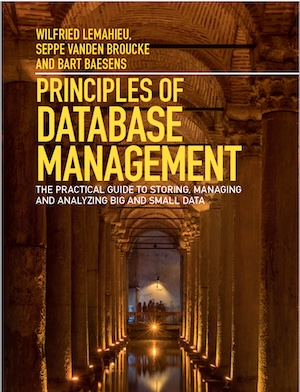
\includegraphics[height=3cm]{images/lemahieu.jpg}\hspace{1cm}
    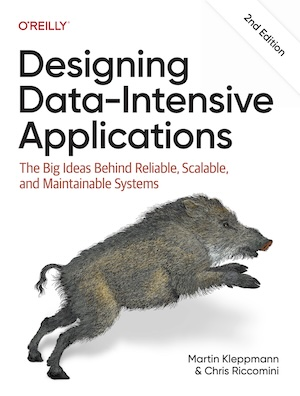
\includegraphics[height=3cm]{images/ddia.jpg}
    \begin{itemize}
        \item Lemahieu, vanden Broucke, and Baesens.\\
            ``\textbf{Principles of Database Management}''.\\
            Cambridge University Press 2018
        \item Kleppmann and Riccomini.\\
            ``\textbf{Designing Data-Intensive Applications}'',\\
            second edition. O’Reilly 2026
    \end{itemize}
    Both are freely available online for Cambridge students.\\
    No need to buy!
\end{frame}
\inlineslide{s:reading}{}

These notes and lectures should be self-contained, but if you would like to read up on further detail, the suggested textbooks are:
\begin{itemize}
    \item Wilfried Lemahieu, Seppe vanden Broucke, and Bart Baesens. \emph{Principles of Database Management}. Cambridge University Press, 2018. ISBN 978-1-107-18612-5

        Free online access from the university network at \url{https://www.cambridge.org/highereducation/books/principles-of-database-management/2FAC1A38D7BF11C3BB1D330925571BE4}

    \item Martin Kleppmann and Chris Riccomini. \emph{Designing Data-Intensive Applications}, second edition. O'Reilly, 2026. ISBN 978-1-098-11906-5

        For free online access, go to \url{https://www.oreilly.com/library/view/designing-data-intensive-applications/9781098119058/} and log in with your \code{@cam.ac.uk} email address.
\end{itemize}

Where appropriate, these lecture notes also contain references to research papers and other useful background reading (these are given in square brackets, and the details appear at the end of this document).
However, only material covered in the lectures, practicals, and/or these notes is examinable.

As for other courses, past exam questions are available at \url{https://www.cl.cam.ac.uk/teaching/exams/pastpapers/t-Databases.html}.
The syllabus, slides, and lecture notes for this course were substantially updated and revised in 2026/27.
Because of syllabus changes, some past exam questions may no longer be applicable.

These notes also contain exercises, which are suggested material for discussion in supervisions.
Solution notes for supervisors are available from the course web page, \courseurl.

\begin{frame}
    \label{s:practicals}
    \frametitle{Databases practicals}
    We provide example databases and practical exercises.\\[1em]
    \textbf{New in 2026/27}: practicals are not formally assessed!\\(No ticks!)\\[1em]
    However:\pause
    \begin{itemize}
        \item Please complete the exercises and discuss them with your supervisor
        \item Feel free to play around with the example databases and try queries of your own
        \item Getting hands-on experience with the practicals is the best exam preparation
        \item Letting AI do the work just harms yourself
    \end{itemize}
\end{frame}
\inlineslide{s:practicals}{}\label{l:practicals}

In previous years, this course included formally assessed practicals (ticks).
That is changing in 2026/27: since AI can now solve any question for you in an instant, we felt that this form of assessment was no longer meaningful.
Instead, this course will be assessed only by the end-of-year exam, like most courses.

We still have practical exercises though, and they are more important than ever!
But rather than formally assessing them, we ask you to complete the exercises in order to support your own learning, and to discuss your solutions with your supervisor.
If you don't complete the practicals, you're missing out on the best possible preparation for the exam, not to mention for your future careers.
You can use AI if you want, but you'd only be cheating yourself out of the education for which you're here.
In the end, that education is your responsibility.


\subsection{What is a database?}\label{sec:what-is-database}

So, what is a database actually?
You can write code that stores data and queries it~-- is that a database?

\begin{frame}
    \label{s:is-this-a-database}
    \frametitle{Is this a database?}
    \inputminted[fontsize=\footnotesize]{python}{code/movies-python.py}\vspace{1em}\pause
    Questions:
    \begin{itemize}
        \item \textbf{Persistence}: what if you restart the program?\pause
        \item \textbf{Sharing}: what if there are many users?\pause
        \item \textbf{Scale}: what if there's more data than fits in memory?\pause
        \item \textbf{Querying}: how do you answer unanticipated questions?\pause
        \item \textbf{Integrity}: what if the computer crashes?
    \end{itemize}
\end{frame}
\inlineslide{s:is-this-a-database}{}\label{l:is-this-a-database}

To answer the questions on \autoref{l:is-this-a-database}:
\begin{itemize}
    \item If you want to be able to make changes to the data and have them persist, even when you restart the program, you have to write them to a file on disk.
    \item If you want to allow several users to simultaneously read and modify the data, you will need some sort of concurrency control, such as locking (see Part IB Concurrent and Distributed Systems).
    \item If you want to handle a dataset that's too big to fit in memory, you will need some way of loading only a part of it at a time.
    \item If you want to allow users to query the data in arbitrary ways, you will need to either let those users edit your program, or have some way of running user code over your data.
    \item If you want to ensure the data doesn't get corrupted in case of a crash, you need careful handling of your writes to disk.
\end{itemize}
These are all things you could program yourself, but a database provides them for you in a convenient package.
We say that the database is a \emph{higher-level abstraction} that lets you store and access your data more conveniently, while handling all of the above issues for you.

Strictly speaking, a database is an organised collection of data; the program that manages it is a \emph{database management system}, or DBMS.
In practice the word ``database'' is used loosely for both, and we will do the same in this course.
The arrangement is shown on \autoref{l:dbms-picture}: applications do not access the bytes on disk directly, but send requests to the DBMS, which manages access to the storage and provides a higher-level abstraction on top of it.

\begin{frame}
    \label{s:dbms-picture}
    \frametitle{The database as abstraction layer}
    \begin{center}
    \begin{tikzpicture}[font=\footnotesize]
        \tikzstyle{app}=[rectangle,rounded corners=2pt,fill=red!10,draw,
            text width=2.2cm,align=center,minimum height=1.0cm]
        \tikzstyle{dbms}=[rectangle,fill=blue!10,draw,
            text width=8.4cm,align=center,minimum height=1.0cm]
        \node [app] (a1) at (0,3.6) {web app};
        \node [app] (a2) at (3.2,3.6) {mobile app};
        \node [app] (a3) at (6.4,3.6) {analytics dashboard};
        \node [dbms] (db) at (3.2,1.7) {\textbf{database management system} (DBMS)};
        % A pair of arrows per application: queries down, results back up, offset 8pt
        % either side of the node's centre. Only the rightmost pair is labelled; three
        % pairs of labels would crowd a gap that is only 1cm deep.
        \foreach \a in {a1,a2,a3} {
            \draw [-{Stealth[length=2mm]},thick]
                ([xshift=-8pt]\a.south) -- ([xshift=-8pt]\a.south |- db.north);
            \draw [-{Stealth[length=2mm]},thick]
                ([xshift=8pt]\a.south |- db.north) -- ([xshift=8pt]\a.south);
        }
        \node [anchor=east] at ([xshift=-12pt,yshift=-0.5cm]a3.south) {queries};
        \node [anchor=west] at ([xshift=12pt,yshift=-0.5cm]a3.south) {results};
        \node (disk) at (3.2,-1) {\storageSymbol};
        \draw [{Stealth[length=2mm]}-{Stealth[length=2mm]},thick]
            (db.south) -- node [right] {reads/writes} (disk);
        \node [anchor=west] at (3.6,-1) {bytes on disk};
    \end{tikzpicture}
    \end{center}
    Every access goes through the DBMS, which can enforce rules, handle concurrent access, and recover from crashes.
\end{frame}
\inlineslide{s:dbms-picture}{}\label{l:dbms-picture}

If your storage needs are simple~-- for example, the data is small and read-only (like a configuration file) or you only need to append to the end (like a log file)~-- using a file is often sufficient, and a database is unnecessary.
But as the data or usage patterns become more complex, databases are indispensable.

The root of the difference is that a file is a sequence of bytes and nothing more.
You can choose a file format, which defines how the file is broken down into values, records, and other structures, but the file system knows nothing about that structure.
In contrast, with a database you generally specify the structure in advance (this is called a \emph{schema}), so the database can ensure that the data conforms to this structure.

Everything else follows from that.
Looking up one record in a file means reading the file from the beginning until you come across it; a database can keep an \emph{index} that allows it to more quickly find the record you're looking for.
Changing a record in the middle of a file means rewriting everything that follows, since the new value rarely occupies exactly the same number of bytes as the old value; databases have more efficient ways of performing small updates to a large dataset.
If the machine loses power halfway through rewriting a file you are left with a file that is neither the old version nor the new one, whereas a database applies a group of changes entirely or not at all, using a concept called a \emph{transaction}.
And two programs writing to one file at the same time will interleave their writes and corrupt the result, unless you build a locking scheme yourself.

None of this is impossible to do with files~-- it is, roughly, what a database does internally~-- but it is a great deal of work to get right, and it is work that has already been done.

\begin{frame}
    \label{s:files-vs-database}
    \frametitle{Why not just use a file?}
    A file gives persistence; a database provides more structure.\\[0.8em]
    \footnotesize
    \rowcolors[]{2}{}{blue!10}
    \renewcommand{\arraystretch}{1.6}
    \begin{tabular}{p{4.85cm}|p{4.85cm}}
        \hline
        \textbf{File} & \textbf{Database} \\\hline
        A sequence of bytes, you define the format
            & Predefined \textbf{schema} that data must conform to \pause\\
        Find a record: read the whole file
            & \textbf{Index}: efficient search for values \pause\\
        Change a record: rewrite everything after it
            & Efficient \textbf{insert, update, delete} of any record \pause\\
        Crash mid-write \newline $\Rightarrow$ corrupted file
            & A \textbf{transaction} applies entirely, or not at all \pause\\
        Two writers at once \newline $\Rightarrow$ corrupted file
            & \textbf{Concurrency control} stops them interfering\pause\\
        A new question: edit the program
            & Write a new \textbf{query} \\\hline
    \end{tabular}
\end{frame}
\inlineslide{s:files-vs-database}{}\label{l:files-vs-database}

Between files and databases sits a widely-used family of systems called \emph{key-value stores}.
A key-value store offers a very simple interface: you can store a value under a key, and retrieve the value for a key.
In return, key-value stores are simple, fast, and comparatively easy to spread across many machines, which is why they are popular for large amounts of data with simple access patterns.

A directory on a filesystem is similar to a key-value store: the filename is the key, the file contents are the value, and the directory gives you a way of listing keys.
The difference is that filesystems are typically designed for larger values (each file is typically assumed to be at least several kilobytes, if not megabytes or gigabytes in size), whereas in a key-value store, values are generally smaller (typically in the low kilobytes, and often just a few bytes).
Also, filesystems often store only a few thousand files per directory and might get slow with more than that, while key-value stores with millions of key-value pairs are common.

\begin{frame}
    \label{s:key-value}
    \frametitle{Key-value stores}
    Two operations: \code{put(key, value)} and \code{get(key)}.\\
    Similar to a Python \code{dict}:
    \inputminted[fontsize=\footnotesize]{python}{code/key-value-python.py}
    \vspace{0.4em}
    \dots{}but it's persistent (on disk) and can be very large.\\[1em]\pause
    You can look up values by key, \textbf{and by nothing else}:
    \begin{itemize}
        \item To the store, keys and values are just bytes
        \item Can't search inside values
        \item Key is some kind of unique identifier (ID)
    \end{itemize}
\end{frame}
\inlineslide{s:key-value}{}\label{l:key-value}

Let's return to the example from \autoref{l:is-this-a-database}.
To find all the movies that came out in 1995, the list comprehension in Python has to scan over all of the movies in the list.
In a database of $n$ movies this has a cost of $O(n)$.
If $n$ is a few thousand this doesn't matter, but it does matter when $n$ is in the millions.

\begin{frame}
    \label{s:full-scan}
    \frametitle{Searching for something that isn't the key}
    Our query from earlier:
    \inputminted[fontsize=\footnotesize]{python}{code/scan-python.py}
    \vspace{0.5em}\pause
    Full scan over all movies.\\
    Cost: $O(n)$ in a database of $n$ movies\\[0.8em]
    Fine for $n = 10^3$, not good for $n = 10^6$.\\[0.8em]
    Key-value stores don't handle this well.
\end{frame}
\inlineslide{s:full-scan}{}\label{l:full-scan}

An \emph{index} is an additional structure, maintained by the database alongside the main data store, that allows you to efficiently find the occurrences of some value~-- like the index at the end of a book, which allows you to find the occurrences of some concept without having to read the entire book.

\autoref{l:indexes} shows what an index could look like if you implemented it using a Python dictionary (which uses a hash table internally).
In fact, most real databases use a sorted structure such as a \emph{B-tree}, which allows lookup with $O(\log n)$ cost, and also supports efficient \emph{range queries}, such as finding all the movies released between 1960 and 1980 \citep{Jones2019}.
See the Algorithms course later this year for more on hash tables and B-trees.

\begin{frame}
    \label{s:indexes}
    \frametitle{Indexes}
    Keep a separate structure containing, for each year, the IDs of movies released in that year:
    \inputminted[fontsize=\footnotesize]{python}{code/index-python.py}
    \vspace{0.4em}
    One lookup in the index, then one per movie ID.\\
    Typically use B-tree for index: lookup cost $O(\log n)$
\end{frame}
\inlineslide{s:indexes}{}\label{l:indexes}

\begin{frame}
    \label{s:index-maintenance}
    \frametitle{Keeping an index up to date}
    Now you have two separate data structures that you have to carefully keep consistent:
    \inputminted[fontsize=\footnotesize]{python}{code/index-maintain-python.py}
    \vspace{0.5em}\pause
    Databases maintain indexes automatically!\\[1em]
    But:
    \begin{itemize}
        \item Index takes space and requires more work on writes
        \item Hence, databases create only explicitly requested indexes
        \item Choosing indexes requires knowledge of query patterns
    \end{itemize}
\end{frame}
\inlineslide{s:index-maintenance}{}\label{l:index-maintenance}

A database management system is what you get when you combine all of the things we discussed: a schema to describe the structure of the data, a query language for asking questions about the data, transactions to avoid corruption due to concurrency or crashes, and indexes for efficient lookups.
The price is that a DBMS is a larger, more complex system.
For use cases that are well served by files or key-value stores, you are better off using those directly.

\begin{frame}
    \label{s:comparison}
    \frametitle{Summary: four ways to keep data}
    \footnotesize
    \rowcolors[]{2}{}{blue!10}
    \renewcommand{\arraystretch}{1.6}
    % Five columns need the inter-column padding halved from its 6pt default to fit the
    % 10.8cm slide: 2.35 + 4 x 1.7 = 9.15cm of columns leaves only ~1.6cm for padding.
    \setlength{\tabcolsep}{3pt}
    \begin{tabular}{>{\raggedright}p{2.35cm}|>{\raggedright}p{1.7cm}|>{\raggedright}p{1.7cm}|>{\raggedright}p{1.7cm}|>{\raggedright\arraybackslash}p{1.7cm}}
        \hline
        & \textbf{Data structure} & \textbf{File} & \textbf{Key-value store} & \textbf{Database} \\\hline
        Persistent across restarts & no & yes & yes & yes \pause\\
        Shared between users & no & awkwardly & yes & yes \pause\\
        Find by key & you code it & you code it & yes & yes \pause\\
        Find by other fields (indexes) & you code it & you code it & no & yes \pause\\
        All-or-nothing updates & no & you code it & sometimes & yes \pause\\
        Checks data consistency & no & no & no & yes \\\hline
    \end{tabular}
\end{frame}
\inlineslide{s:comparison}{}\label{l:comparison}

\subsection{Types of databases}\label{sec:database-types}

There are many different types of databases designed for different purposes.
To choose the one that is most appropriate to the problem you are trying to solve, you need to know the ways they are commonly categorised.

The first way in which databases are distinguished is by their \emph{data model}: the expected shape of your data.
A \emph{relational} database holds tables of rows and columns, with rows in one table referring to rows in another by key.
The relational model was introduced by \citet{Codd1970} and has been the most popular model for the last half century, so we focus most on it in this course.
But there are also alternatives: a \emph{document} database holds self-contained documents, usually encoded as JSON, in which related information is nested inside the document rather than being split across tables.
A \emph{graph} database holds vertices joined by edges, and is optimised for following those edges from one vertex to the next.
(Graphs are introduced in more detail in the Algorithms course later this year.)
The same information can generally be represented in any of these data models, but often one of them is more convenient than the others.

Beyond these three there are databases specialised for particular kinds of data: time series from sensors, vectors for AI applications, geospatial data such as geographic maps, and a variety of data formats used for scientific applications such as climate models, telescope images, and many others.
They are outside the scope of this course, but it's worth knowing that they exist.

\begin{frame}
    \label{s:data-models}
    \frametitle{Data models}
    % One model per overlay, with visible on=<n->, which hides an element while still
    % counting it in the bounding box, so nothing moves as the slide builds.
    %
    % The descriptions used to be a tabular beneath the picture, which had to be aligned
    % with it by hand. They are nodes in the picture now, at the same three x positions as
    % the panels, so the alignment is automatic. The move was forced as well as tidy:
    % wrapping a p{} cell in \onslide (or \uncover, or \visible) makes it 10.15pt taller,
    % which \arraystretch 1.6 turned into a 16.24pt gap between the two rows.
    \begin{center}
    \begin{tikzpicture}
        \tikzstyle{icon}=[draw,thick,fill=blue!8]
        \tikzstyle{desc}=[anchor=north west,text width=3.2cm,align=left]
        % relational: a grid with a shaded header row
        \begin{scope}[visible on=<1->]
            \fill [blue!25] (0,0.9) rectangle (2.4,1.2);
            \draw [icon] (0,0) rectangle (2.4,1.2);
            \foreach \y in {0.3,0.6,0.9} \draw (0,\y) -- (2.4,\y);
            \foreach \x in {0.8,1.6} \draw (\x,0) -- (\x,1.2);
        \end{scope}
        % document: fields nested inside a record
        \begin{scope}[visible on=<2->,shift={(3.5,0)}]
            \draw [icon,rounded corners=3pt] (0,0) rectangle (2.4,1.2);
            \draw [fill=blue!25,rounded corners=2pt] (0.2,0.85) rectangle (1.5,1.05);
            \draw [fill=blue!25,rounded corners=2pt] (0.2,0.15) rectangle (2.2,0.7);
            \draw [fill=blue!45,rounded corners=2pt] (0.45,0.25) rectangle (1.3,0.45);
            \draw [fill=blue!45,rounded corners=2pt] (1.45,0.25) rectangle (2.0,0.45);
        \end{scope}
        % graph: vertices joined by edges
        \begin{scope}[visible on=<3->,shift={(7.0,0)}]
            \tikzstyle{v}=[circle,draw,thick,fill=blue!25,minimum size=0.42cm,inner sep=0pt]
            \node [v] (n1) at (0.45,0.95) {};
            \node [v] (n2) at (1.75,1.05) {};
            \node [v] (n3) at (0.85,0.25) {};
            \node [v] (n4) at (2.1,0.3) {};
            \foreach \a/\b in {n1/n2,n1/n3,n3/n4,n2/n4}
                \draw [-{Stealth[length=1.5mm]},thick] (\a) -- (\b);
        \end{scope}
        \node [anchor=north west,visible on=<1->] at (0,-0.15) {\textbf{Relational}};
        \node [anchor=north west,visible on=<2->] at (3.5,-0.15) {\textbf{Document}};
        \node [anchor=north west,visible on=<3->] at (7.0,-0.15) {\textbf{Graph}};
        \node [desc,visible on=<1->] at (0,-0.8)   {Tables with rows and columns};
        \node [desc,visible on=<2->] at (3.5,-0.8) {JSON: records nested inside one another};
        \node [desc,visible on=<3->] at (7.0,-0.8) {Vertices joined by edges};
        \node [desc,visible on=<1->] at (0,-2.635)   {e.g.\ PostgreSQL, SQLite, DuckDB};
        \node [desc,visible on=<2->] at (3.5,-2.635) {e.g.\ MongoDB, CouchDB};
        \node [desc,visible on=<3->] at (7.0,-2.635) {e.g.\ Neo4j, Memgraph};
    \end{tikzpicture}
    \end{center}
    \onslide<4->{Also: time series, vectors, geospatial, scientific arrays\dots}
\end{frame}
\inlineslide{s:data-models}{}\label{l:data-models}

Another way in which we distinguish databases is in terms of where the database runs.

An \emph{embedded} database is a library that runs inside your own program, in the same process, reading and writing a file on the same machine.
This approach works well for apps that only need to store data on behalf of the local user.
SQLite is a popular example (used in many mobile apps), and DuckDB (which we use in this course) is another.

A \emph{client-server} database runs as a separate process, usually on a separate machine, and one or more programs connect to it over a network.
This is convenient for services that are accessed from many different devices, such as a website.
PostgreSQL and MySQL are common choices of client-server databases, but many others also exist.

A \emph{distributed} database spreads the data over many machines, so that both the storage and the work of querying it are shared.
This approach is needed when the amount of data is too big to hold on a single machine.
Systems like Snowflake and BigQuery are used by large corporations to store large volumes of data for analytical purposes.
For example, a supermarket chain might store every single purchase made by customers (with date, time, shop location, price, etc.), allowing them to analyse the effect of running a particular promotion.
Such datasets can grow to be petabytes ($10^{15}$ bytes) in size.
A database designed for such business analytics is also known as a \emph{data warehouse}.

\begin{frame}
    \label{s:deployment}
    \frametitle{Where the database runs}
    \tikzset{
        app/.style={draw,thick,rounded corners=2pt,fill=red!10,font=\scriptsize,
            minimum width=1.5cm,minimum height=0.5cm,inner sep=2pt},
        srv/.style={draw,thick,fill=blue!10,font=\scriptsize,
            minimum width=1.5cm,minimum height=0.5cm,inner sep=2pt},
        lnk/.style={-{Stealth[length=1.5mm]},thick}}
    \textbf{Embedded} (SQLite, DuckDB) \hfill megabytes to gigabytes\\[0.2em]
    \begin{tikzpicture}
        \draw [draw,thick,rounded corners=2pt,fill=red!10] (0,-0.45) rectangle (3.6,0.45);
        \node [anchor=west,font=\scriptsize] at (0.1,0.25) {your program};
        \node [srv] at (2.5,-0.1) {DB};
        \node [scale=0.5] at (4.4,-0.15) {\storageSymbol};
        \draw [lnk] (3.3,-0.1) -- (4.2,-0.1);
    \end{tikzpicture}\\[1em]\pause
    \textbf{Client-server} (PostgreSQL, MySQL) \hfill gigabytes to terabytes\\[0.2em]
    \begin{tikzpicture}
        \node [app] (a1) at (0.75,0.35) {program};
        \node [app] (a2) at (0.75,-0.35) {program};
        \node [srv] (s)  at (3.3,0) {server};
        \draw [lnk] (a1) -- (s); \draw [lnk] (a2) -- (s);
        \node [scale=0.5] at (4.9,-0.05) {\storageSymbol};
        \draw [lnk] (s) -- (4.7,0);
    \end{tikzpicture}\\[1em]\pause
    \textbf{Distributed} (Snowflake, BigQuery) \hfill terabytes to petabytes\\[0.2em]
    \begin{tikzpicture}
        \node [app] (a) at (0.75,0) {program};
        \foreach \y/\n in {0.6/s1,0/s2,-0.6/s3} {
            \node [srv] (\n) at (3.3,\y) {server};
            \draw [lnk] (a) -- (\n);
            \node [scale=0.45] at (4.8,\y-0.05) {\storageSymbol};
            \draw [lnk] (\n) -- (4.6,\y);
        }
    \end{tikzpicture}
\end{frame}
\inlineslide{s:deployment}{}\label{l:deployment}

Yet another way of distinguishing databases is in terms of their internal data layout.
A database's data model presents a \emph{logical} representation of the data, and this is the level at which you write queries.
On the other hand, the \emph{physical} representation is how the bytes are actually arranged on disk and in memory, and it has a big impact on the performance of the database.
The separation between these two representations allows the physical representation to be changed without affecting the logical representation: the same data can be stored in different ways, and queries continue giving the same answers.
This property is called \emph{data independence}.

\begin{frame}
    \label{s:row-column}
    \frametitle{Row-oriented and column-oriented}
    % The three excerpts come from examples/layout-*.sql, which read the same two movies
    % out of the database as a table, laid out row by row, and laid out column by column.
    %
    % Built up one layout at a time with visible on=<n->, which hides an element while
    % still counting it in the bounding box. A plain \node<n-> does not: the picture would
    % then be 5.24cm wide on the first overlay and 9.76cm on the last, and the whole thing
    % would slide as it built. Hand-declaring \useasboundingbox also works in principle,
    % but the numbers are easy to get wrong -- the two layout nodes are wide and centred
    % on points well inside the span they occupy -- and getting them wrong moves the
    % picture off centre without any warning from the build.
    \begin{center}
    \begin{tikzpicture}
        \tikzstyle{lg}=[font=\footnotesize,rectangle,fill=red!8,draw,thick,inner sep=5pt]
        \tikzstyle{ph}=[rectangle,fill=blue!8,draw,thick,align=left,
            font=\ttfamily\footnotesize,inner sep=5pt]
        \node [anchor=south,visible on=<1->] at (4.3,4.0) {the same \textbf{logical} table\dots};
        \node [lg,visible on=<1->] (tbl) at (4.3,3.0) {% The same two movies as a logical table, for the logical/physical diagram
% Generated from layout-logical.sql by examples/render.py -- do not edit.
% Regenerate with: make examples
\begin{tabular}{l|l|r}\hline
    \textbf{movie\_id} & \textbf{title} & \textbf{year} \\\hline
    \texttt{tt0012349} & The Kid & 1921 \\
    \texttt{tt0078748} & Alien & 1979 \\\hline
\end{tabular}%
};
        \node [anchor=south,visible on=<2->] at (4.3,1.3) {\dots two \textbf{physical} layouts};
        \node [ph,visible on=<2->] (row) at (1.6,0.4) {% Two movies laid out row by row, for the logical/physical diagram
% Generated from layout-row.sql by examples/render.py -- do not edit.
% Regenerate with: make examples
tt0012349|The Kid|1921\\ tt0078748|Alien|1979%
};
        \node [ph,visible on=<3->] (col) at (7.2,0.4) {% The same two movies laid out column by column, for the logical/physical diagram
% Generated from layout-column.sql by examples/render.py -- do not edit.
% Regenerate with: make examples
tt0012349,tt0078748\\ The Kid,Alien\\ 1921,1979%
};
        \node [anchor=north,visible on=<2->] at (1.6,-0.35) {\textbf{row-oriented}};
        \node [anchor=north,visible on=<3->] at (7.2,-0.35) {\textbf{column-oriented}};
        \draw [-{Stealth[length=2mm]},thick,visible on=<2->] (tbl.south west) -- (row.north);
        \draw [-{Stealth[length=2mm]},thick,visible on=<3->] (tbl.south east) -- (col.north);
    \end{tikzpicture}
    \end{center}
    \onslide<4->{Often update individual records $\Rightarrow$ row-oriented is better\\
    Often summarise many records $\Rightarrow$ column-oriented is better}
\end{frame}
\inlineslide{s:row-column}{}\label{l:row-column}

For databases with a relational model, there are two common physical representations.
A \emph{row-oriented} database stores each row as one contiguous run of bytes.
A \emph{column-oriented} database stores the values from each column together instead, so that reading one column of a million rows touches only the bytes of that column, and values of the same type sit next to each other and compress well \citep{Abadi2013}.

Which is better depends on the workload.
As a rule of thumb, if you most often read or write one or a few rows at a time (known as \emph{OnLine Transaction Processing} or OLTP), a row-oriented layout tends to be better.
If you often read large numbers of rows at a time, and also load data in large batches (as is typical in \emph{analytics}), a column-oriented database often performs better.
For example, the database behind a website (where you can make a post, a purchase, etc.) is typically optimised for OLTP, whereas a data warehouse (as in the supermarket example) is designed for analytics.

Each data model comes with a query language, and this course covers several of them.
\emph{SQL} is the language of relational databases, and by far the most widely used; most of this course is about it.
SQL is one of the world's most popular programming languages \citep{Caballar2022}.
But we will also look at several alternatives that are better in some circumstances.

\begin{frame}
    \label{s:query-languages}
    \frametitle{Query languages covered in this course}
    \textbf{SQL} (Structured Query Language)
    \begin{itemize}
        \item Very popular, you have to know it
        \item Originally relational, but extensions for JSON, XML, graphs, etc.\ have been added
        \item Corresponds roughly to \textbf{relational algebra}\\[1em]\pause
    \end{itemize}
    \textbf{Datalog}
    \begin{itemize}
        \item Also relational, much less well known
        \item Learn it to understand recursive queries\\[1em]\pause
    \end{itemize}
    \textbf{SQL/PGQ} (graphs)
    \begin{itemize}
        \item $\approx$ Cypher, absorbed into SQL\\[1em]\pause
    \end{itemize}
    \textbf{JSON} (documents)
    \begin{itemize}
        \item Not a query language per se, but a useful data model
    \end{itemize}
\end{frame}
\inlineslide{s:query-languages}{}\label{l:query-languages}

All of the query languages we study in this course are \emph{declarative} \citep{Krishnaswami2013}.
That is, the query describes only what is wanted, but it doesn't say what algorithm should be used to compute the query result.
Thus, the DBMS is free to pick whatever algorithm it believes will be fastest; for example, it can automatically choose which indexes to use to answer the query.
The \emph{query optimiser} is the component within the DBMS that makes these choices; it produces a \emph{query plan} for a query, which then tells the DBMS engine how to execute the query.

\begin{frame}
    \label{s:declarative}
    \frametitle{Declarative languages}
    SQL and the other query languages in this course are \textbf{declarative}:
    \inputminted[fontsize=\footnotesize]{sql}{code/declarative-sql.sql}
    \vspace{0.6em}
    Describe the properties of the data you want; not how to compute it.
    Database automatically chooses indexes to use.\\[1em]\pause
    % Both Python lines are repeated verbatim from code/scan-python.py and
    % code/index-python.py, so that the slide is recognisably the earlier examples.
    In Python you write an \textbf{algorithm} to compute the data:
    \inputminted[fontsize=\footnotesize]{python}{code/declarative-python.py}
    \vspace{0.6em}
    To start using an index you have to rewrite the algorithm.
\end{frame}
\inlineslide{s:declarative}{}\label{l:declarative}

\supervision{\label{q:declarative}
    What are some advantages and disadvantages of a declarative query language compared to a general-purpose programming language such as Python?
}{
    Advantages:
    \begin{itemize}
        \item The query is often more succinct and easier to write, since algorithmic details don't need to be specified.
        \item Queries can sometimes be made faster by adding an index to the database, without having to rewrite the queries themselves.
        \item New versions of the DBMS can introduce new algorithms and optimisations that automatically improve query performance, without requiring any changes to queries.
            The query optimiser can make sophisticated decisions based on the statistical distribution of the data, its physical data layout, what is in the cache, etc.~-- information that may not be known at the time of writing the query.
        \item Large queries can be speeded up automatically by executing them in parallel across multiple CPU cores and across multiple machines.
            Such automatic parallelisation is much harder in general-purpose programming languages, and it is essential in large (petabyte-scale) data warehouses.
    \end{itemize}
    Disadvantages:
    \begin{itemize}
        \item Declarative languages are generally less expressive: they are good if you're doing the things that the language was designed to do, but if the language doesn't support the operation you need, there often isn't a good way of implementing it yourself.
        \item Users rely on the query optimiser making good choices.
            If the query optimiser is not very good, performance can be worse than if the users had more control over the execution.
        \item Writing a good query optimiser is very hard, requiring many years of engineering effort.
        \item The performance of queries can change unexpectedly.
            For example, if the statistical distribution of the data has changed gradually, at some point the query optimiser may suddenly switch an existing query to a new query plan, which can cause disruption if the new query plan has worse performance than the old one.
    \end{itemize}
    Overall, declarative queries reduce complexity for users of the database, but increase the complexity of the DBMS internals.
    They are an example of an abstraction that hides the underlying DBMS complexity.
}

\section{Relational data modelling}\label{sec:relational}

\begin{frame}
    \begin{center}
        {\Large{\color{darkblue}{Relational data modelling}}} \\[2em]
        \mydetails
    \end{center}
\end{frame}

Throughout this course we will use one running example: a database of movies.
You can run every query in these notes for yourself, and experiment with different queries in order to get a feel for using different data models and query languages.
\autoref{l:running-duckdb} explains how to get it running.

The data is a subset of the IMDb non-commercial datasets~\citep{IMDb:2025}.
The full dataset is too large to be convenient, so we have filtered it down to roughly \dbapproxmovies\ popular movies: enough that queries return interesting results, but small enough that the whole database runs comfortably on a laptop.
For now we will look at a relational representation of the dataset, and we will consider other data models later.

\begin{frame}
    \label{s:moviedb-intro}
    \frametitle{Our running example: a movies database}
    A subset of the IMDb public datasets:
    \begin{itemize}
        \item $\approx$\dbapproxmovies\ movies, $\approx$\dbapproxpeople\ cast and crew members
        \item Small enough to run on a laptop, big enough to be interesting
        \item Incomplete (e.g.\ missing people), real-world messiness\\[1em]\pause
    \end{itemize}
    Download it yourself; query and modify it as you like!\\
    (Instructions in the notes)\\[1em]
    We will use the same dataset with different data models and query languages to compare those approaches.
\end{frame}
\inlineslide{s:moviedb-intro}{}\label{l:moviedb-intro}

The database consists of seven tables, listed on \autoref{l:moviedb-tables}.
The tables fall into two groups.
Three of them~-- \code{movies}, \code{people}, and \code{genres}~-- each describe a kind of \emph{thing} in the world: a movie, a person, a genre.
We will call these \emph{entity tables}.
The others describe \emph{relationships} between those things: which movie has which genre, which person worked on which movie, and so on.
This distinction is not part of SQL~-- to the database, all seven are simply tables~-- but it is a useful way to read a schema, and we will return to it when we look at how to design one.

\begin{frame}
    \label{s:moviedb-tables}
    \frametitle{Tables in the movies database}
    A relational database stores everything in tables:\\[1em]
    {\footnotesize
    \rowcolors[]{2}{}{blue!10}
    \renewcommand{\arraystretch}{1.3}
    % The \tikzmark commands record row positions for the braces drawn below; see setup.tex.
    \begin{tabular}{l|p{4.6cm}|r}
        \hline
        \textbf{table} & \textbf{one row per\dots} & \textbf{rows} \\\hline
        \code{movies}        & movie                      & \dbrowsmovies \tikzmark{entfirst}\\
        \code{people}        & member of cast or crew     & \dbrowspeople \\
        \code{genres}        & genre name                 & \dbrowsgenres \tikzmark{entlast}\pause\\
        \code{ratings}       & movie's average rating     & \dbrowsratings \\
        \code{has_genre}    & movie paired with a genre  & \dbrowshasgenre \tikzmark{relfirst}\\
        \code{has_position} & job someone held on a movie & \dbrowshasposition \\
        \code{plays_role}   & character an actor played  & \dbrowsplaysrole \tikzmark{rellast}\pause\\\hline
    \end{tabular}}%
    % Braces spanning the two groups of rows. Drawn top-to-bottom so that the brace
    % bulges to the right, i.e. renders as a closing brace. The vertical offsets put the
    % ends 1pt inside the top of the first and the bottom of the last row of each group.
    % The relationships brace deliberately starts at has_genre, leaving the ratings row
    % between the two braces: ratings is not a relationship between two entities, which
    % is left to be explained in the lecture rather than on the slide.
    \begin{tikzpicture}[remember picture,overlay]
        \tikzset{grouplabel/.style={rotate=90,font=\footnotesize,inner sep=0pt}}
        \draw<3-> [decorate,decoration={brace,amplitude=6pt}]
            ([xshift=12pt,yshift=9.9pt]entfirst) -- ([xshift=12pt,yshift=-3.7pt]entlast);
        \node<3-> [grouplabel] at ([xshift=27pt,yshift=-12.5pt]entfirst) {entities};
        \draw<3-> [decorate,decoration={brace,amplitude=6pt}]
            ([xshift=12pt,yshift=9.9pt]relfirst) -- ([xshift=12pt,yshift=-3.7pt]rellast);
        \node<3-> [grouplabel] at ([xshift=27pt,yshift=-12.5pt]relfirst) {relationships};
    \end{tikzpicture}\\[1em]
    \textbf{Entities}: ``things'' in the world\\
    \textbf{Relationships}: how one entity relates to another\\[1em]
    Both entities and relationships are represented as tables
\end{frame}
\inlineslide{s:moviedb-tables}{}\label{l:moviedb-tables}

Every table has a \emph{primary key}: a column, or a combination of columns, whose value identifies a row uniquely.
It is common for primary keys to simply be integers, but in our example database, the keys of \code{movies} and \code{people} are the string identifiers that IMDb itself uses: movies have keys like \code{tt0012349} and people have keys like \code{nm0000122}.
A key like this, which already exists in the data and has a meaning outside the database, is called a \emph{natural key}.
The \code{genres} table is different: IMDb records genres only as names, but our database assigns an integer \code{genre_id} to each of the \dbrowsgenres\ genres.
A key invented purely to identify rows is called a \emph{surrogate key}.

\autoref{l:primary-key} shows a few rows of two of the tables, with the primary key of each marked.

\begin{frame}
    \label{s:primary-key}
    \frametitle{Primary keys}
    A \textbf{primary key} identifies a row uniquely:\\
    no two rows of a table may hold the same value in it.
    \par\vspace{0.6em}
    {\footnotesize\centering
    \begin{tabular}{@{}c@{\hspace{1.5cm}}c@{}}
        \textbf{movies} & \textbf{genres} \\[0.3em]
        % A three-row excerpt of movies, for the primary key slide
% Generated from pk-movies.sql by examples/render.py -- do not edit.
% Regenerate with: make examples
\begin{tabular}{|l|l|r|}\hline
    \tikzmarknode{pkm0}{\textbf{movie\_id}} & \textbf{title} & \textbf{year} \\\hline
    \tikzmarknode{pkm1}{\texttt{tt0078748}} & Alien & 1979 \\
    \tikzmarknode{pkm2}{\texttt{tt0120338}} & Titanic & 1997 \\
    \tikzmarknode{pkm3}{\texttt{tt6751668}} & Parasite & 2019 \\\hline
\end{tabular}%
 & % A three-row excerpt of genres, for the primary key slide
% Generated from pk-genres.sql by examples/render.py -- do not edit.
% Regenerate with: make examples
\begin{tabular}{|r|l|}\hline
    \tikzmarknode{pkg0}{\textbf{genre\_id}} & \textbf{name} \\\hline
    \tikzmarknode{pkg1}{22} & Sci-Fi \\
    \tikzmarknode{pkg2}{21} & Romance \\
    \tikzmarknode{pkg3}{8} & Drama \\\hline
\end{tabular}%

    \end{tabular}\\[3em]}
    % Braces under the key columns. Drawn right-to-left, which is the direction that makes
    % the brace bulge downwards; fit= spans the column from its header to its last row.
    \begin{tikzpicture}[remember picture,overlay]
        \tikzset{keybrace/.style={decorate,decoration={brace,amplitude=5pt},thick},
                 keylabel/.style={midway,below=8pt,font=\footnotesize}}
        \node [fit=(pkm0)(pkm3),inner sep=0pt] (pkmcol) {};
        \node [fit=(pkg0)(pkg3),inner sep=0pt] (pkgcol) {};
        \draw<2-> [keybrace] ([yshift=-4pt]pkmcol.south east) -- ([yshift=-4pt]pkmcol.south west)
            node [keylabel] {primary key};
        \draw<2-> [keybrace] ([yshift=-4pt]pkgcol.south east) -- ([yshift=-4pt]pkgcol.south west)
            node [keylabel] {primary key};
    \end{tikzpicture}%
    \uncover<2->{\code{movie_id} is a string; \code{genre_id} is an integer.\\
    Either is fine, as long as it is unique.\\[0.5em]}%
    \uncover<3->{A primary key may consist of several columns\\
    (\textbf{composite primary key}) $\Longrightarrow$ values in all those columns combined must be unique}
\end{frame}
\inlineslide{s:primary-key}{}\label{l:primary-key}

Where one table needs to refer to a row of another, it stores that row's primary key in a column of its own, and declares it as a \emph{foreign key}.
For example, each row of \code{has_genre} holds a \code{movie_id} and a \code{genre_id}, which refer to rows of \code{movies} and \code{genres} respectively.

\autoref{l:foreign-key} shows this happening: every value in the \code{has_genre} excerpt is the primary key of a row in one of the other two tables.

\begin{frame}
    \label{s:foreign-key}
    \frametitle{Foreign keys}
    A \textbf{foreign key} holds the primary key of a row in another table.
    % has_genre is placed between the two tables it refers to, and the genres table is
    % indented so that its key column sits under the genre_id column of has_genre. The
    % values the overlay joins up are then on the facing edges of adjacent tables, so the
    % lines are short and cross no cell text. See the ordering note in the .sql files.
    \par\vspace{0.6em}
    {\footnotesize\centering
    % The description column is 2.6cm and the gutters 0.25cm because the row holding the
    % indented genres table sets the middle column's width: caption 47.5pt + gutter +
    % 2.1cm + genres 104pt + gutter + description must stay inside \textwidth = 307.3pt.
    \begin{tabular}{@{}r@{\hspace{0.25cm}}l@{\hspace{0.25cm}}>{\raggedright\arraybackslash}m{2.6cm}@{}}
        \textbf{movies}     & % The movies excerpt again, for the foreign key slide
% Generated from fk-movies.sql by examples/render.py -- do not edit.
% Regenerate with: make examples
\begin{tabular}{|l|l|r|}\hline
    \tikzmarknode{fkm0}{\textbf{movie\_id}} & \textbf{title} & \textbf{year} \\\hline
    \tikzmarknode{fkm1}{\texttt{tt0078748}} & Alien & 1979 \\
    \tikzmarknode{fkm2}{\texttt{tt0120338}} & Titanic & 1997 \\
    \tikzmarknode{fkm3}{\texttt{tt6751668}} & Parasite & 2019 \\\hline
\end{tabular}%
    & \\[1.0cm]
        \textbf{has\_genre} & % has_genre rows referring only to the movies and genres shown on the same slide
% Generated from fk-has-genre.sql by examples/render.py -- do not edit.
% Regenerate with: make examples
\begin{tabular}{|l|r|}\hline
    \tikzmarknode{fkhm0}{\textbf{movie\_id}} & \tikzmarknode{fkhg0}{\textbf{genre\_id}} \\\hline
    \tikzmarknode{fkhm1}{\texttt{tt6751668}} & \tikzmarknode{fkhg1}{8} \\
    \tikzmarknode{fkhm2}{\texttt{tt0120338}} & \tikzmarknode{fkhg2}{8} \\
    \tikzmarknode{fkhm3}{\texttt{tt0120338}} & \tikzmarknode{fkhg3}{21} \\
    \tikzmarknode{fkhm4}{\texttt{tt0078748}} & \tikzmarknode{fkhg4}{22} \\\hline
\end{tabular}%
 & % The has_genre excerpt read out in words, for the foreign key slide
% Generated from fk-has-genre-words.sql by examples/render.py -- do not edit.
% Regenerate with: make examples
``Alien'' is Sci-Fi; ``Titanic'' is Drama and Romance; ``Parasite'' is Drama%
 \\[1.0cm]
        \textbf{genres}     & \hspace{2.1cm}% The genres excerpt again, for the foreign key slide
% Generated from fk-genres.sql by examples/render.py -- do not edit.
% Regenerate with: make examples
\begin{tabular}{|r|l|}\hline
    \tikzmarknode{fkg0}{\textbf{genre\_id}} & \textbf{name} \\\hline
    \tikzmarknode{fkg1}{22} & Sci-Fi \\
    \tikzmarknode{fkg2}{21} & Romance \\
    \tikzmarknode{fkg3}{8} & Drama \\\hline
\end{tabular}%
 &
    \end{tabular}\par}
    % fit= puts an ellipse round a marked cell; a line between two ellipse nodes is
    % clipped to their borders automatically.
    \begin{tikzpicture}[remember picture,overlay]
        % fill opacity keeps the value legible under the shading; no shorten=, so the
        % line runs from one ellipse's border to the other's with no gap.
        \tikzset{circled/.style={draw,thick,ellipse,inner sep=2pt,fill opacity=0.2},
                 joiner/.style={thick}}
        \node<2-> [circled,red,fill=red]           (cmA) [fit=(fkm3)]  {};
        \node<2-> [circled,red,fill=red]           (cmB) [fit=(fkhm1)] {};
        \draw<2-> [joiner,red]                     (cmA) -- (cmB);
        \node<3-> [circled,darkblue,fill=darkblue] (cgA) [fit=(fkhg4)] {};
        \node<3-> [circled,darkblue,fill=darkblue] (cgB) [fit=(fkg1)]  {};
        \draw<3-> [joiner,darkblue]                (cgA) -- (cgB);
    \end{tikzpicture}
\end{frame}
\inlineslide{s:foreign-key}{}\label{l:foreign-key}

A primary key does not have to be a single column.
The primary key of \code{has_genre} is the pair \code{(movie_id, genre_id)}, and it has to be: as \autoref{l:composite-key} shows, neither column on its own takes a different value in every row.
A movie appears once for each of its genres, and a genre once for each movie that has it, so only the two columns \emph{together} identify a row.
A key made of several columns like this is called a \emph{composite primary key}.

\begin{frame}
    \label{s:composite-key}
    \frametitle{Composite primary keys}
    In \code{has_genre}, neither column is unique on its own.
    \par\vspace{0.6em}
    {\footnotesize\centering
    % The has_genre excerpt once more, for the composite primary key slide
% Generated from ck-has-genre.sql by examples/render.py -- do not edit.
% Regenerate with: make examples
\begin{tabular}{|l|r|}\hline
    \tikzmarknode{ckhm0}{\textbf{movie\_id}} & \tikzmarknode{ckhg0}{\textbf{genre\_id}} \\\hline
    \tikzmarknode{ckhm1}{\texttt{tt6751668}} & \tikzmarknode{ckhg1}{8} \\
    \tikzmarknode{ckhm2}{\texttt{tt0120338}} & \tikzmarknode{ckhg2}{8} \\
    \tikzmarknode{ckhm3}{\texttt{tt0120338}} & \tikzmarknode{ckhg3}{21} \\
    \tikzmarknode{ckhm4}{\texttt{tt0078748}} & \tikzmarknode{ckhg4}{22} \\\hline
\end{tabular}%
\par}
    \vspace{0.75cm}
    \begin{tikzpicture}[remember picture,overlay]
        \tikzset{circled/.style={draw,thick,ellipse,inner sep=2pt,fill opacity=0.2},
                 keybrace/.style={decorate,decoration={brace,amplitude=5pt},thick},
                 keylabel/.style={midway,below=8pt,font=\footnotesize}}
        \node [circled,red,fill=red,fit=(ckhm2)] {};
        \node [circled,red,fill=red,fit=(ckhm3)] {};
        \node [circled,darkblue,fill=darkblue,fit=(ckhg1)] {};
        \node [circled,darkblue,fill=darkblue,fit=(ckhg2)] {};
        % Brace under both columns at once: fit over all four corner cells of the table.
        \node [fit=(ckhm0)(ckhg0)(ckhm4)(ckhg4),inner sep=0pt] (ckcol) {};
        \draw<2-> [keybrace] ([yshift=-4pt]ckcol.south east) -- ([yshift=-4pt]ckcol.south west)
            node [keylabel] {primary key};
    \end{tikzpicture}\\[0.5em]
    \code{movie_id} repeats: one movie can have several genres.\\
    \code{genre_id} repeats: one genre applies to several movies.\\[0.5em]%
    \uncover<2->{But \code{(movie_id, genre_id)} together are unique.\\[1em]}%
    \uncover<3->{It's also okay for a table not to have any primary key.\\
    Then it may contain duplicate rows.}
\end{frame}
\inlineslide{s:composite-key}{}\label{l:composite-key}

\autoref{l:moviedb-schema} shows the whole schema drawn as a diagram, with an arrow from each foreign key to the primary key it references.
A diagram like this is the quickest way to get your bearings in an unfamiliar database.
The colour-coding is not standard, but it's a common convention to underline the columns that form the primary key.

\begin{frame}[plain]
    \label{s:moviedb-schema}
    \frametitle{The movie database schema}
    \begin{center}
    \begin{tikzpicture}[font=\scriptsize]
        \tikzstyle{tbl}=[rectangle split,rectangle split parts=2,draw,thick,
            text width=2.15cm,align=left,inner sep=3pt]
        \tikzstyle{entity}=[tbl,rectangle split part fill={red!30,red!8}]
        \tikzstyle{jointbl}=[tbl,rectangle split part fill={blue!25,blue!8}]
        \tikzstyle{fk}=[-{Stealth[length=2.2mm]},thick]
        \tikzstyle{card}=[font=\tiny,inner sep=3pt]
        \useasboundingbox (-0.1,-0.15) rectangle (10.65,6.75);

        % Entity tables
        \node<1-> [entity] (genres) at (1.3,5.9)
            {\textbf{genres}\nodepart{second}\ttfamily\underline{genre\_id}\\name};
        \node<1-> [entity] (movies) at (5.0,3.3)
            {\textbf{movies}\nodepart{second}\ttfamily\underline{movie\_id}\\title\\year\\type\\minutes};
        \node<1-> [entity] (people) at (8.6,5.9)
            {\textbf{people}\nodepart{second}\ttfamily\underline{person\_id}\\name\\birthyear\\deathyear};

        % Relationship tables
        \node<3-> [jointbl] (ratings) at (5.0,5.9)
            {\textbf{ratings}\nodepart{second}\ttfamily\underline{movie\_id}\\rating\\votes};
        \node<2-> [jointbl] (hasgenre) at (1.3,3.3)
            {\textbf{has\_genre}\nodepart{second}\ttfamily\underline{movie\_id}\\\underline{genre\_id}};
        \node<4-> [jointbl] (haspos) at (8.6,3.3)
            {\textbf{has\_position}\nodepart{second}\ttfamily\underline{movie\_id}\\\underline{person\_id}\\\underline{position}\\job};
        \node<5-> [jointbl] (playsrole) at (8.6,0.75)
            {\textbf{plays\_role}\nodepart{second}\ttfamily\underline{movie\_id}\\\underline{person\_id}\\\underline{role}};

        % Foreign keys
        \draw<3-> [fk] (ratings.south)   -- node [card,left,pos=0.12]  {$1$} node [card,left,pos=0.88]  {$1$} (movies.north);
        \draw<2-> [fk] (hasgenre.north)  -- node [card,left,pos=0.12]  {$N$} node [card,left,pos=0.88]  {$1$} (genres.south);
        \draw<2-> [fk] (hasgenre.east)   -- node [card,above,pos=0.12] {$N$} node [card,above,pos=0.88] {$1$} (movies.west);
        \draw<4-> [fk] (haspos.west)     -- node [card,above,pos=0.12] {$N$} node [card,above,pos=0.88] {$1$} (movies.east);
        \draw<4-> [fk] (haspos.north)    -- node [card,right,pos=0.12] {$N$} node [card,right,pos=0.88] {$1$} (people.south);
        \draw<5-> [fk] (playsrole.west)  -- node [card,above,pos=0.06] {$N$} (5.0,0.75) -- node [card,right,pos=0.8] {$1$} (movies.south);
        \draw<5-> [fk] (playsrole.east)  -- node [card,above,pos=0.3]  {$N$} (10.35,0.75) -- (10.35,5.9) -- node [card,above,pos=0.75] {$1$} (people.east);

        % Legend
        \draw<1-> [thick,fill=red!8]  (0.25,1.65) rectangle +(0.4,0.28);
        \node<1-> [anchor=west,font=\scriptsize] at (0.75,1.79) {entity table};
        \draw<1-> [thick,fill=blue!8] (0.25,1.05) rectangle +(0.4,0.28);
        \node<1-> [anchor=west,font=\scriptsize] at (0.75,1.19) {relationship table};
        \draw<1-> [fk] (0.25,0.59) -- (0.65,0.59);
        \node<1-> [anchor=west,font=\scriptsize] at (0.75,0.59) {foreign key};
        \node<1-> [anchor=west,font=\scriptsize] at (0.10,0.02) {\underline{underlined} = part of the primary key};
    \end{tikzpicture}
    \end{center}%
\end{frame}
\inlineslide{s:moviedb-schema}{}\label{l:moviedb-schema}

\noindent The \code{movies} table has one row per movie:
\begin{itemize}
    \item \code{movie_id}: a unique identifier (chosen by IMDb), which serves as the primary key.
    \item \code{title}: the movie's title; it is not unique, since different movies can have the same title.
    \item \code{year}: the year of release.
    \item \code{type}: one of % The distinct values of movies.type, most common first
% Generated from movie-types.sql by examples/render.py -- do not edit.
% Regenerate with: make examples
\texttt{movie}, \texttt{tvMovie}, or \texttt{video}%
, distinguishing a cinema release from one made for television or released direct to video.
    \item \code{minutes}: the running time in minutes.
\end{itemize}
The \code{people} table has one row per member of a cast or crew:
\begin{itemize}
    \item \code{person_id}: a unique identifier (chosen by IMDb), and the primary key.
    \item \code{name}: the person's name.
    \item \code{birthyear}: the year of birth (\code{NULL} where IMDb records none, which is the case for \dbnullbirthyear\% of people).
    \item \code{deathyear}: the year of death, \code{NULL} for \dbnulldeathyear\% of people.
        A \code{NULL} here means either that the person is still alive or that no date has been recorded, and the database does not distinguish between the two.
\end{itemize}
The \code{genres} table has one row per genre name:
\begin{itemize}
    \item \code{genre_id}: a unique integer identifier, which serves as the primary key.
    \item \code{name}: the name of the genre, such as \code{Comedy} or \code{Documentary}.
\end{itemize}
The \code{ratings} table has one row per movie:
\begin{itemize}
    \item \code{movie_id}: the ID of the movie being rated; both a foreign key to \code{movies} and the primary key of this table.
    \item \code{rating}: the average of the scores IMDb users have given the movie, out of ten.
    \item \code{votes}: the number of scores that average was calculated from.
\end{itemize}
The \code{has_genre} table has one row for each pairing of a movie with a genre.
It has two columns that together form its primary key:
\begin{itemize}
    \item \code{movie_id}: the ID of the movie being described; a foreign key to \code{movies}.
    \item \code{genre_id}: the ID of the genre attached to that movie; a foreign key to \code{genres}.
\end{itemize}
The \code{has_position} table has one row for each job that a person held on a movie.
Its primary key consists of three of the four columns: \code{person_id}, \code{movie_id}, and \code{position}.
\begin{itemize}
    \item \code{person_id}: the ID of the person; a foreign key to \code{people}.
    \item \code{movie_id}: the ID of the movie; a foreign key to \code{movies}.
    \item \code{position}: what the person did, one of % The distinct values of has_position.position, most common first
% Generated from positions.sql by examples/render.py -- do not edit.
% Regenerate with: make examples
\texttt{actor}, \texttt{producer}, \texttt{writer}, \texttt{composer}, or \texttt{director}%
.
    \item \code{job}: for some positions, extra details on the job they did, such as ``written by'' or ``co-producer''.
        \code{NULL} for positions that do not have this extra detail, or where none was provided.
\end{itemize}
The \code{plays_role} table has one row for each character that an actor played, with all three columns forming the primary key:
\begin{itemize}
    \item \code{person_id}: the ID of the person; a foreign key to \code{people}.
    \item \code{movie_id}: the ID of the movie; a foreign key to \code{movies}.
    \item \code{role}: the name of the character, as IMDb records it.
\end{itemize}

One caveat applies to all of these tables.
IMDb's data is incomplete, and this database is a filtered subset of it, so a cast member you expect to find may simply be absent, and two movies you expect to be connected through a shared collaborator may have no connection in the data.

% label= (beamer's, not \label) lets \againframe repeat this slide in sec:documents.
\begin{frame}[label=moviedb-kid1]
    \label{s:moviedb-kid1}
    \frametitle{One movie across the tables (1/2)}
    \footnotesize
    \textbf{movies}\\[0.2em]
    % The Kid's row in the movies table
% Generated from kid-movies.sql by examples/render.py -- do not edit.
% Regenerate with: make examples
\begin{tabular}{|l|l|r|l|r|}\hline
    \textbf{movie\_id} & \textbf{title} & \textbf{year} & \textbf{type} & \textbf{minutes} \\\hline
    \texttt{tt0012349} & The Kid & 1921 & movie & 68 \\\hline
\end{tabular}%
\\[1em]
    \textbf{ratings}\\[0.2em]
    % The Kid's row in the ratings table
% Generated from kid-ratings.sql by examples/render.py -- do not edit.
% Regenerate with: make examples
\begin{tabular}{|l|r|r|}\hline
    \texttt{tt0012349} & 8.2 & 142,991 \\\hline
\end{tabular}%
\\[1em]
    \textbf{has\_genre}\hspace{2.655cm}\textbf{genres}\\[0.2em]
    % The Kid's rows in the has_genre table
% Generated from kid-has-genre.sql by examples/render.py -- do not edit.
% Regenerate with: make examples
\begin{tabular}{|l|r|}\hline
    \textbf{movie\_id} & \textbf{genre\_id} \\\hline
    \texttt{tt0012349} & 5 \\
    \texttt{tt0012349} & 8 \\
    \texttt{tt0012349} & 11 \\\hline
\end{tabular}%
\hspace{1em}%
    % The genres rows referenced by The Kid
% Generated from kid-genres.sql by examples/render.py -- do not edit.
% Regenerate with: make examples
\begin{tabular}{|r|l|}\hline
    \textbf{genre\_id} & \textbf{name} \\\hline
    5 & Comedy \\
    8 & Drama \\
    11 & Family \\\hline
\end{tabular}%

\end{frame}
\inlineslide{s:moviedb-kid1}{}\label{l:moviedb-kid1}

\begin{frame}[label=moviedb-kid2]
    \label{s:moviedb-kid2}
    \frametitle{One movie across the tables (2/2)}
    {\footnotesize
    \textbf{people}\\[0.2em]
    % Charles Chaplin's row in the people table
% Generated from chaplin-people.sql by examples/render.py -- do not edit.
% Regenerate with: make examples
\begin{tabular}{|l|l|r|r|}\hline
    \textbf{person\_id} & \textbf{name} & \textbf{birthyear} & \textbf{deathyear} \\\hline
    \texttt{nm0000122} & Charles Chaplin & 1889 & 1977 \\\hline
\end{tabular}%
\\[1em]
    \textbf{has\_position}\\[0.2em]
    % Charles Chaplin's rows in has_position for The Kid
% Generated from chaplin-has-position.sql by examples/render.py -- do not edit.
% Regenerate with: make examples
\begin{tabular}{|l|l|l|l|}\hline
    \textbf{person\_id} & \textbf{movie\_id} & \textbf{position} & \textbf{job} \\\hline
    \texttt{nm0000122} & \texttt{tt0012349} & actor & \textit{null} \\
    \texttt{nm0000122} & \texttt{tt0012349} & composer & composer \\
    \texttt{nm0000122} & \texttt{tt0012349} & director & director \\
    \texttt{nm0000122} & \texttt{tt0012349} & producer & producer \\
    \texttt{nm0000122} & \texttt{tt0012349} & writer & written by \\\hline
\end{tabular}%
\\[1em]
    \textbf{plays\_role}\\[0.2em]
    % Charles Chaplin's rows in plays_role for The Kid
% Generated from chaplin-plays-role.sql by examples/render.py -- do not edit.
% Regenerate with: make examples
\begin{tabular}{|l|l|l|}\hline
    \textbf{person\_id} & \textbf{movie\_id} & \textbf{role} \\\hline
    \texttt{nm0000122} & \texttt{tt0012349} & A Tramp \\\hline
\end{tabular}%
\\[1em]}
\end{frame}
\inlineslide{s:moviedb-kid2}{}\label{l:moviedb-kid2}

\autoref{l:moviedb-kid1} and \ref{l:moviedb-kid2} show a sample of the actual data, following a single movie through the tables.
\emph{The Kid} is one row of \code{movies}, with the key \code{tt0012349}, and one row of \code{ratings} carrying its score.
Its three genres appear as three rows of \code{has_genre}, each pairing the movie's key with a genre's key, so reading the genre \emph{names} requires looking up those keys in \code{genres}.
Charles Chaplin is one row of \code{people}, and his five positions on the movie are five rows of \code{has_position}, plus one row of \code{plays_role} for the character he played.
Note how the movie's title appears exactly once in the whole database, and Chaplin's name exactly once, no matter how many rows refer to them.
Storing each fact in exactly one place is a central concern of relational design, and we will look at it properly when we come to \emph{normalisation} in \autoref{sec:normalisation}.

The tables are created with the SQL \code{CREATE TABLE} statements shown on \autoref{l:moviedb-ddl1} and \ref{l:moviedb-ddl2}.
This part of SQL, which defines the structure of the data rather than reading or changing it, is called the \emph{data definition language} (DDL).
Each column is given a name and a type, and the \code{PRIMARY KEY} and \code{REFERENCES} clauses declare the keys that we read off the diagram.
Where the primary key consists of a single column it can be declared on that column; where it spans several columns it needs a separate \texttt{PRIMARY KEY (\dots)} clause.

% The SQL in code/movies-entities.sql and code/movies-relationships.sql is extracted verbatim
% from the CREATE TABLE statements in moviedb-generator/make_databases.py (which are one-liners
% there), reformatted across several lines to fit on a slide. Verified character-identical to the
% generator modulo whitespace, and identical to the schema of the example database.
% Row counts and example rows on these slides were read from that same database file.
\begin{frame}
    \label{s:moviedb-ddl1}
    \frametitle{Creating the entity tables in SQL}
    \inputminted[fontsize=\scriptsize]{sql}{code/movies-entities.sql}
\end{frame}
\inlineslide{s:moviedb-ddl1}{}\label{l:moviedb-ddl1}

\begin{frame}[plain]
    \label{s:moviedb-ddl2}
    \frametitle{Creating the relationship tables in SQL}
    \inputminted[fontsize=\scriptsize]{sql}{code/movies-relationships.sql}
\end{frame}
\inlineslide{s:moviedb-ddl2}{}\label{l:moviedb-ddl2}

A foreign key declaration is not merely documentation: it is a constraint that the database can enforce.
If \code{has_genre} contains a \code{movie_id} that does not appear in \code{movies}, the reference points at nothing, and the database is said to have lost \emph{referential integrity}.
A database system that enforces foreign keys will refuse any insert, update, or delete that would leave a dangling reference.
DuckDB, which is what we are using, does enforce them, but SQLite, for example, ignores foreign key declarations unless \code{PRAGMA foreign_keys = ON} is specified.
Thus, despite SQL being standardised, you can still find significant variations in behaviour between systems.

Primary and foreign keys are commonly used to construct three different types of relationship, as shown on \autoref{l:relationship-types}.

\begin{frame}
    \label{s:relationship-types}
    \frametitle{Three shapes of relationship}
    \tikzset{
        tbl/.style={rectangle split,rectangle split parts=2,draw,thick,
            text width=1.55cm,align=left,inner sep=3pt,font=\scriptsize},
        entity/.style={tbl,rectangle split part fill={red!30,red!8}},
        jointbl/.style={tbl,rectangle split part fill={blue!25,blue!8}},
        fk/.style={-{Stealth[length=2.2mm]},thick},
        card/.style={font=\tiny,inner sep=3pt}}
    \textbf{one-to-one}: {\footnotesize a movie has at most one rating}\\[0.25em]
    \begin{tikzpicture}
        \node [entity]  (m1) at (1.2,0) {\textbf{movies}\nodepart{second}\ttfamily\underline{movie\_id}};
        \node [jointbl] (r1) at (4.2,0) {\textbf{ratings}\nodepart{second}\ttfamily\underline{movie\_id}};
        \draw [fk] (r1.west) -- node [card,above,pos=0.08] {$1$} node [card,above,pos=0.92] {$1$} (m1.east);
    \end{tikzpicture}\\\pause

    \textbf{many-to-many}: {\footnotesize a movie has many genres, a genre many movies}\\[0.25em]
    \begin{tikzpicture}
        \node [entity]  (m2) at (1.2,0) {\textbf{movies}\nodepart{second}\ttfamily\underline{movie\_id}};
        \node [jointbl] (h2) at (4.2,0) {\textbf{has\_genre}\nodepart{second}\ttfamily\underline{movie\_id}\\\underline{genre\_id}};
        \node [entity]  (g2) at (7.2,0) {\textbf{genres}\nodepart{second}\ttfamily\underline{genre\_id}};
        \draw [fk] (h2.west) -- node [card,above,pos=0.08] {$N$} node [card,above,pos=0.92] {$1$} (m2.east);
        \draw [fk] (h2.east) -- node [card,above,pos=0.08] {$N$} node [card,above,pos=0.92] {$1$} (g2.west);
    \end{tikzpicture}\\\pause

    \textbf{one-to-many}: {\footnotesize a series contains many movies}\\[0.25em]
    \begin{tikzpicture}
        \node [entity] (s3) at (1.2,0) {\textbf{series}\nodepart{second}\ttfamily\underline{series\_id}};
        \node [entity] (m3) at (4.2,0) {\textbf{movies}\nodepart{second}\ttfamily\underline{movie\_id}\\series\_id};
        \draw [fk] (m3.west) -- node [card,above,pos=0.08] {$N$} node [card,above,pos=0.92] {$1$} (s3.east);
    \end{tikzpicture}\\
    {\footnotesize Adding \code{series} to the example database is an exercise}
\end{frame}
\inlineslide{s:relationship-types}{}\label{l:relationship-types}

You can tell what kind of relationship it is by looking at the primary key of each table.
The \code{ratings} table has \code{movie_id} as its entire primary key, and that column is also a foreign key to \code{movies}.
Since a primary key value can appear only once, this means each movie has at most one row in the \code{ratings} table, and each rating belongs to exactly one movie: a \emph{one-to-one} relationship.

\supervision{\label{q:ratings-separate}
    Instead of having a separate \code{ratings} table, another way of making a one-to-one relation would be to add \code{rating} and \code{votes} as columns of the \code{movies} table.
    What are the pros and cons of these approaches?
    Think about how the tables might be used by an application, how you might enforce constraints, and how future-proof each approach is.
}{
    Arguments for a separate table:
    \begin{itemize}
        \item It allows the relationship to be partial: if a movie has no votes, a separate table simply has no row for that movie, whereas columns in \code{movies} would have to be filled with nulls or placeholder values.
        \item The two tables have different update patterns.
            Ratings change continuously as people vote, whereas a movie's title, year, and duration very rarely change.
            Keeping them apart means a rating update does not touch the \code{movies} row, which can improve performance for updates.
        \item If you wanted to record ratings from different sources~-- say, a critics' score, or the rating from another site~-- you could add a \code{source} column to the \code{ratings} table's primary key, and then store one rating per source per movie as a row in the \code{ratings} table.
            If you use columns on the \code{movies} table, you would need to add separate columns for each source, which would quickly become messy.
            (However, this would arguably change the one-to-one relationship into a many-to-many relationship between movies and sources.)
        \item The rating is arguably a fact about how the public received the movie rather than a property of the movie itself, so it can make sense to model it separately.
    \end{itemize}
    Arguments for columns on the \code{movies} table:
    \begin{itemize}
        \item A query that wants a rating alongside a title needs to only read from one table rather than two, which is simpler and faster than reading from two tables.
        \item If it has a \code{NOT NULL} constraint, that ensures there is exactly one rating per movie.
            With a separate table, there could be zero or one ratings per movie.
    \end{itemize}
}

In a \emph{many-to-many} relationship like the \code{has_genre} table, both columns are foreign keys, and the primary key contains both columns.
A table like this, whose only purpose is to connect rows of two other tables, is called an \emph{associative table} or \emph{join table}.
Many-to-many relationships cannot be represented by putting a foreign key in either of the two entity tables, so a third table is the standard solution.

The \code{has_position} and \code{plays_role} tables represent many-to-many relationships with extra information about the relationship.
In the \code{has_position} table, the primary key is \code{(movie_id, person_id, position)}, which means that the same person may hold several positions on the same movie: Charles Chaplin has % How many positions Charles Chaplin held on The Kid
% Generated from chaplin-positions-count.sql by examples/render.py -- do not edit.
% Regenerate with: make examples
5%
 rows for \emph{The Kid}, since he acted in it, directed it, produced it, wrote it, and composed its music.
Had the primary key been just \code{(movie_id, person_id)}, that would have been impossible to record.
The \code{job} column then holds IMDb's free-text description of the position (``written by'', ``co-producer''), and is null in % Percentage of has_position rows whose job is null (the % sign is added in databases.tex)
% Generated from null-jobs.sql by examples/render.py -- do not edit.
% Regenerate with: make examples
68%
\% of rows.
Similarly, \code{plays_role} has primary key \code{(movie_id, person_id, role)}, so an actor can play more than one character in a movie; this occurs % How many (movie, person) pairs play more than one character
% Generated from multi-role-people.sql by examples/render.py -- do not edit.
% Regenerate with: make examples
1,007%
 times in the example database.

\begin{frame}
    \label{s:moviedb-shapes}
    \frametitle{Reading the shape off the primary key}
    \footnotesize
    \rowcolors[]{2}{}{blue!10}
    \renewcommand{\arraystretch}{1.3}
    \begin{tabular}{l|>{\raggedright}p{3.8cm}|>{\raggedright\arraybackslash}p{3.1cm}}
        \hline
        \textbf{table} & \textbf{primary key} & \textbf{relationship} \\\hline
        \code{ratings} & \code{movie_id} \newline (one foreign key) & one-to-one \pause\\
        \code{has_genre} & \code{(movie_id, genre_id)} \newline (two foreign keys) & many-to-many \pause\\
        \code{has_position} & \code{(movie_id, person_id, position)} & many-to-many, \newline with attributes \\
        \code{plays_role} & \code{(movie_id, person_id, role)} & many-to-many, \newline with attributes \\\hline
    \end{tabular}\\[1em]
    \code{position} is in the key $\Longrightarrow$ one person can hold \textbf{several} positions on the same movie.\\[0.4em]\pause
    To make a \textbf{one-to-many} relationship:\\
    A foreign key column that is not part of the primary key, and no join table.
    See exercise in the notes.
\end{frame}
\inlineslide{s:moviedb-shapes}{}\label{l:moviedb-shapes}

There is no example of a \emph{one-to-many} relationship in the example database, but we could add one.
Suppose we wanted to record which series or franchise a movie belongs to, so that, say, the \emph{Star Wars} films form one series and the \emph{Lord of the Rings} trilogy another.
A series contains many movies, and a movie belongs to at most one series, which gives us a one-to-many relationship between series and movies.

\supervision{\label{q:one-to-many}
    Give the SQL statements that you would use to change the example database to add the concept of a series of movies.
    You can add a column to an existing table using the \code{ALTER TABLE} statement; see the \href{https://duckdb.org/docs/lts/sql/statements/alter_table}{DuckDB documentation} for details.
    How would you record a movie's position within its series (e.g.\ being part 1, 2, or 3 of a trilogy)?
    Can you prevent two movies from being given the same position within their series?
}{
    A series is a thing in its own right, so it needs an entity table with a surrogate key.
    The reference to it then goes into \code{movies}:
    \inputminted[fontsize=\small]{sql}{code/series.sql}
    A few points to note:
    \begin{itemize}
        \item The foreign key goes on the ``many'' side (the \code{movies} table in this case).
            A series contains many movies, so the series' key is repeated across many \code{movies} rows; a movie belongs to one series, so a single column in \code{movies} is enough to hold the reference.
            Putting a \code{movie_id} column in \code{series} would allow only one movie per series, which is the wrong way round.
        \item \code{series_id} is not part of the primary key of \code{movies}.
            That ensures that a movie's ID is unique, but multiple movies can have the same \code{series_id}.
        \item No join table~-- a third table is needed only for many-to-many relationships.
        \item Most movies do not belong to any series, so \code{series_id} is null for many rows.
            That is desirable: a nullable foreign key is how we say that a row may or may not be related to another entity.
    \end{itemize}
    To enforce the foreign key constraint, we ought to declare \code{REFERENCES series(series_id)} on the new column, but unfortunately DuckDB does not yet support adding foreign key constraints to an existing table (other SQL databases allow this).
    To get around that limitation in DuckDB you could create a fresh \code{movies} table with the constraint, copy the rows across, and swap the two tables.

    A movie's position within its series is a property of neither the movie alone nor the series alone, but of the movie's membership of that series.
    Since the membership is recorded by the \code{series_id} column of the row in the \code{movies} table, the position belongs in that table too, as a further column~-- \code{series_index}, say.
    Adding \code{UNIQUE (series_id, series_index)} would then stop two movies claiming the same position in one series.
    A further subtlety with ordering within a series is that the \emph{Star Wars} films were not released in the order of their episode numbers, so release order and episode order differ, and the schema has to either pick one of the two orderings, or record both.

    If a movie could belong to two series~-- a crossover between them, say~-- then this would be a many-to-many relationship, and a join table would be needed:
    \inputminted[fontsize=\small]{sql}{code/in-series.sql}
}

% Commented out because it's perhaps too hard...

% \supervision{
%     Suppose you want the database to guarantee that a person can only play a character in a movie if they are also recorded as an actor on that movie~-- that is, every row of \code{plays_role} has a matching row in \code{has_position} with \code{position = 'actor'}.
%     Can this be expressed as a foreign key constraint on the schema as it stands?
%     If not, how could the schema be changed so that it can be?
% }{
%     It cannot be expressed as a foreign key on the current schema.
%     A foreign key must reference the primary key (or another uniquely-constrained set of columns) of the target table.
%     The primary key of \code{has_position} is \code{(movie_id, person_id, position)}, so a foreign key from \code{plays_role} would have to supply all three columns, and \code{plays_role} has no \code{position} column.
%     Adding \code{(movie_id, person_id)} as a foreign key would not work either, since that pair is not unique in \code{has_position}~-- the whole point of including \code{position} in the key is that a person may hold several positions on one movie.
%
%     One clean fix is to give \code{plays_role} a \code{position} column that is constrained to the value \code{'actor'}, and then declare a three-column foreign key:
%     \begin{itemize}
%         \item add \code{position TEXT CHECK (position = 'actor')} to \code{plays_role};
%         \item declare\\
%             \code{FOREIGN KEY (movie_id, person_id, position)}\\
%             \code{REFERENCES has_position(movie_id, person_id, position)}.
%     \end{itemize}
%     This works, at the cost of a column whose value is always the same, which is redundant.
%
%     A tidier alternative is to restructure: give \code{has_position} a surrogate primary key (say \code{position_id}), keep a uniqueness constraint on \code{(movie_id, person_id, position)}, and have \code{plays_role} reference \code{position_id} instead of the movie and person separately.
%     A row of \code{plays_role} then hangs off exactly one position, and the constraint that it must be an \code{actor} position is the only part left for a \code{CHECK} or a trigger to enforce.
%     This also removes the duplication of \code{movie_id} and \code{person_id} between the two tables.
%
%     It is worth noticing what this exercise shows in general: the set of constraints a relational schema can enforce declaratively is limited, and expressing a rule sometimes requires changing the structure of the tables rather than just adding a constraint.
%     Rules that cannot be expressed either move into triggers, or become the application's responsibility.
% }


\supervision{\label{q:position-tables}
    Every type of relationship that a person may have with a movie~-- acting, directing, producing, writing, composing~-- is recorded in one table, \code{has_position}, with a \code{position} column saying which type each row is.
    An alternative design would be to create a separate table for each type of relationship: \code{directs}, \code{produces}, \code{composes}, and so on.
    How would you decide which of these approaches to use?
}{
    The single table is better whenever the different types of relationship are treated alike:
    \begin{itemize}
        \item A query that does not care which type of relationship it is (e.g.\ looking up everyone who worked on a given movie, or every movie a given person worked on) only needs to read from one table.
            Using a separate table per relationship type makes the query more complicated.
        \item Adding a new relationship type is easier: just insert rows with the new type, and no schema change is necessary.
            Adding a new table is a schema change, which is harder, and any queries that need to consider all relationship types need to be modified.
    \end{itemize}

    Separate tables are better when the relationship types are \emph{not} alike, which arguably is the case in our example database.
    In the example database there is some variation between the different types of position:

    \begin{quote}% Rows per position, and how many of them fill in the job column
% Generated from position-job.sql by examples/render.py -- do not edit.
% Regenerate with: make examples
\begin{tabular}{|l|r|r|}\hline
    \textbf{position} & \textbf{rows} & \textbf{with a job} \\\hline
    \texttt{actor} & 29,153 & 0 \\
    \texttt{producer} & 7,429 & 7,429 \\
    \texttt{writer} & 6,782 & 6,647 \\
    \texttt{composer} & 3,281 & 1,148 \\
    \texttt{director} & 3,166 & 731 \\\hline
\end{tabular}%
\end{quote}

    \begin{itemize}
        \item With a table per relationship type, those tables can have different columns, whereas in the single-table approach you need to fill in nulls for values that don't apply.
            For example, in the movie database, the \code{job} column means something different for each type of relationship, and nothing at all for actors: it is null for every one of the actor rows and filled in for every producer row.
        \item With multiple tables you can express constraints that apply to only one type of relationship.
            With a single table, you would need a constraint that is conditional on the \code{position} value.
        \item With multiple tables, the set of possible relationship types is enforced by the schema rather than by convention.
            In a single table, if you make the type a free-form string, the database cannot catch typos.
            (In the example database, the \code{job} column contains \qcountdistinctjobs\ distinct values, including both \code{screenplay by} and \code{screen play by}, demonstrating the problem with an uncontrolled vocabulary.)

            This can be addressed by defining the column to be an enum type, which allows it to take only one of a set of specified values, or by defining a \code{position_types} table and making \code{position} a foreign key into that table.
        \item Queries about one specific type of relationship are simpler and faster when each type of relationship has its own table.
    \end{itemize}
}


\section{SQL and relational algebra}\label{sec:sql}

\begin{frame}
    \begin{center}
        {\Large{\color{darkblue}{SQL and relational algebra}}} \\[2em]
        \mydetails
    \end{center}
\end{frame}

We've seen some examples of SQL already, but now let's explore it a bit more systematically.
SQL is a large and complex language, and we will not be able to cover all of it in this course.
However, knowing the core ideas of SQL is essential for working with relational databases.

The best way of learning SQL is not just to read these notes, but also to try everything yourself.
We will use DuckDB for SQL, so please get the example database of movies from the course web page, \courseurl.

See \url{https://duckdb.org/install/?environment=cli} for instructions on installing the DuckDB command line interface on your own machine.
You should then be able to simply run \code{duckdb movies.duckdb} where \code{movies.duckdb} is the name of the database file you downloaded from the course web page.
Alternatively, you can run DuckDB inside your web browser without installing anything at all.

Either way, you have your own copy of the database that is not shared with any other student.
Therefore, feel free to do anything you want with the database, including deleting all of the data.
If you break the database file, you can always re-download it from the course web page.
The browser version does not save changes at all: if you reload the tab, the database is reset to its original state.

These notes only give an outline of the SQL language; for full details please refer to the \href{https://duckdb.org/docs/current/sql/introduction}{DuckDB documentation}.

\begin{frame}
    \label{s:running-duckdb}
    \frametitle{Running SQL yourself}
    You can use DuckDB in two ways:
    \begin{itemize}
        \item \textbf{On your own machine}:
            \begin{itemize}
                \item Install DuckDB from duckdb.org
                \item Download the database file from the course web page
                \item If you break it, just re-download it\\[0.5em]\pause
            \end{itemize}
        \item \textbf{In your web browser} 
            \begin{itemize}
                \item Nothing to install, go to course web page
                \item Nothing is saved when you reload the tab\\[1em]
            \end{itemize}
    \end{itemize}
    You have your own copy: feel free to break it!\\
    Nobody else is affected.\\[1em]\pause
    Please check the \textbf{DuckDB documentation} for language details
\end{frame}
\inlineslide{s:running-duckdb}{}\label{l:running-duckdb}

\begin{frame}
    \label{s:sql-parts}
    \frametitle{Overview of SQL}
    \begin{itemize}
        \item \textbf{Data Definition Language} (DDL)
            \begin{itemize}
                \item \code{CREATE TABLE}, \code{ALTER TABLE}, \code{DROP TABLE}
                \item \code{CREATE INDEX}, \dots
                \item Describes the \textbf{schema} of the database\\[1em]\pause
            \end{itemize}
        \item \textbf{Data Manipulation Language} (DML)
            \begin{itemize}
                \item \code{INSERT}, \code{UPDATE}, \code{DELETE}
                \item \code{BEGIN TRANSACTION}, \code{COMMIT}, \code{ROLLBACK}
                \item Changes the data in the database\\[1em]\pause
            \end{itemize}
        \item \textbf{Queries}
            \begin{itemize}
                \item \code{SELECT}: Asks questions about the data\\[1em]
            \end{itemize}
    \end{itemize}
    We will also cover \textbf{relational algebra}
    \begin{itemize}
        \item Mathematical notation approximately equivalent to SQL queries (\code{SELECT})
    \end{itemize}
\end{frame}
\inlineslide{s:sql-parts}{}\label{l:sql-parts}

Alongside SQL we will introduce \emph{relational algebra}, which is a small mathematical notation that corresponds roughly to the core concepts in SQL.
Although we don't normally use relational algebra to write queries in practice, it is a useful tool for defining what relational queries actually \emph{mean}, and query optimisers typically use a form of relational algebra internally when planning how to execute a query.

A \emph{relation}, the fundamental building block of relational algebra, is a set of tuples.
For now you can think of it as the set of rows in a table, and we will refine this idea later.
The Part IA Discrete Maths course offers a more formal introduction to relations.

\subsection{Defining and manipulating data}

Let's start with DDL.
We have already seen examples of it: the \code{CREATE TABLE} statements on \autoref{l:moviedb-ddl1}.
A \code{CREATE TABLE} statement names the table, then lists its columns, each with a name and a type, and any constraints.

The types in our example database are simple: \code{INT} for integers, \code{TEXT} for strings, \code{NUMERIC} (a fixed-point decimal number) for the ratings.
Many more types exist: dates, times, booleans, floating-point numbers, JSON, arrays, and more~-- though their support varies considerably between different DBMSs.

\begin{frame}
    \label{s:ddl}
    \frametitle{Data definition language: \code{CREATE TABLE}}
    \inputminted[fontsize=\footnotesize]{sql}{code/ddl-create.sql}
    \vspace{0.5em}\pause
    A column has a \textbf{name} and a \textbf{type}. A table may also have
    \textbf{constraints} that the database will not let you violate:
    \begin{itemize}
        \item \code{PRIMARY KEY} -- identifies a row; at most one row per value
        \item \code{REFERENCES} -- a foreign key; must name a row that exists
        \item \code{NOT NULL}, \code{UNIQUE}, \code{CHECK}, \dots
    \end{itemize}
\end{frame}
\inlineslide{s:ddl}{}\label{l:ddl}

\begin{frame}
    \label{s:ddl-alter}
    \frametitle{Changing and removing tables}
    \inputminted[fontsize=\footnotesize]{sql}{code/ddl-alter.sql}
    \vspace{1em}\pause
    \textbf{Schema migration}: changing the schema of an existing database\\[1em]
    Problems: can require rewriting table (slow); queries written against the old schema may stop working
\end{frame}
\inlineslide{s:ddl-alter}{}\label{l:ddl-alter}

DDL also covers indexes.
On \autoref{l:indexes} we saw an index \code{movies_by_year} built from a second Python dictionary, which you needed to manually keep consistent with \code{movies_by_id} (\autoref{l:index-maintenance}).
In SQL, indexes are much easier to work with: you only need to once declare what index you want using \code{CREATE INDEX}, and then the database automatically keeps the index up-to-date for you.

\begin{frame}
    \label{s:create-index}
    \frametitle{Creating and deleting indexes}
    \inputminted[fontsize=\footnotesize]{sql}{code/ddl-index.sql}
    \vspace{0.8em}
    Declare it once; the database automatically maintains and uses the index thereafter.\\[0.8em]\pause
    An index does not change query \textbf{results}, only \textbf{performance}.\\[0.8em]
    A \code{PRIMARY KEY} or \code{UNIQUE} constraint usually creates an index implicitly.
    (The index is needed to check uniqueness.)
\end{frame}
\inlineslide{s:create-index}{}\label{l:create-index}

\begin{frame}
    \label{s:dml}
    \frametitle{Inserting, updating, and deleting rows}
    \inputminted[fontsize=\footnotesize]{sql}{code/dml.sql}
    \vspace{1em}\pause
    \raisebox{-2pt}{
\includegraphics[height=12pt]{images/26a0.pdf}} 
    \code{UPDATE} and \code{DELETE} apply to every row matching the \code{WHERE} clause.
    If you leave out the \code{WHERE}, they apply to \textbf{every row} in the table!
\end{frame}
\inlineslide{s:dml}{}\label{l:dml}

\subsection{Querying a single table}

The \code{SELECT} statement in SQL is used to query the database.
We will start off with simple \code{SELECT} statements and work our way up to more complex ones.
Let's start by reading a whole table: \code{SELECT * FROM movies} fetches every column of every row.
The \code{*} means ``all columns''; \code{movies} is the table to read.

\begin{frame}
    \label{s:select-all}
    \frametitle{Fetching all rows from one table}
    \inputminted[fontsize=\footnotesize]{sql}{code/sel-1-all.sql}
    \vspace{0.3em}
    {\scriptsize% SELECT * FROM movies, truncated to fit a slide
% Generated from sel-all.sql by examples/render.py -- do not edit.
% Regenerate with: make examples
\begin{tabular}{|l|l|r|l|r|}\hline
    \textbf{movie\_id} & \textbf{title} & \textbf{year} & \textbf{type} & \textbf{minutes} \\\hline
    \texttt{tt0012349} & The Kid & 1921 & movie & 68 \\
    \texttt{tt0015324} & Sherlock Jr. & 1924 & movie & 45 \\
    \texttt{tt0015864} & The Gold Rush & 1925 & movie & 95 \\
    \texttt{tt0017136} & Metropolis & 1927 & movie & 153 \\
    $\vdots$ & $\vdots$ & $\vdots$ & $\vdots$ & $\vdots$ \\\hline
\end{tabular}%
}\\[0.8em]
    All \dbrowsmovies\ rows in arbitrary order, all five columns.\\[1em]\pause
    Use \code{LIMIT} if you want fewer rows:
    \inputminted[fontsize=\footnotesize]{sql}{code/sel-2-limit.sql}
    \vspace{0.3em}
    {\scriptsize% SELECT * FROM movies LIMIT 4
% Generated from sel-limit.sql by examples/render.py -- do not edit.
% Regenerate with: make examples
\begin{tabular}{|l|l|r|l|r|}\hline
    \textbf{movie\_id} & \textbf{title} & \textbf{year} & \textbf{type} & \textbf{minutes} \\\hline
    \texttt{tt0012349} & The Kid & 1921 & movie & 68 \\
    \texttt{tt0015324} & Sherlock Jr. & 1924 & movie & 45 \\
    \texttt{tt0015864} & The Gold Rush & 1925 & movie & 95 \\
    \texttt{tt0017136} & Metropolis & 1927 & movie & 153 \\\hline
\end{tabular}%
}\\[0.8em]
    Note: Since the order of rows is not defined, this might give you \textbf{any three} rows, not three specific ones
\end{frame}
\inlineslide{s:select-all}{}\label{l:select-all}

Nothing in that query says anything about the order of the rows.
A relation is a \emph{set} of rows (strictly speaking, a multiset~-- more on this in \autoref{sec:algebra-sql}), and a set has no order, so the database is free to return the rows in whatever order it finds most convenient.
It may return them in one order today, and a different order tomorrow.
If you want a particular order you have to ask for it using an \code{ORDER BY} clause in the \code{SELECT} statement.
If you combine \code{ORDER BY} with \code{LIMIT} $n$, the database will first sort the rows and then return the first $n$ of the sorted result.

You can choose to sort either in ascending order, from smallest to largest value (the default), or in descending order from largest to smallest by putting the \code{DESC} keyword after the column name.
You can sort by more than one column, as on \autoref{l:order-by}: the second column is consulted only when the value in the first is equal, the third only where the first two are equal, and so on.

\begin{frame}
    \label{s:order-by}
    \frametitle{Ordering rows: \code{ORDER BY}}
    \inputminted[fontsize=\footnotesize]{sql}{code/sel-3-order.sql}
    \vspace{0.3em}
    {\scriptsize% the same with ORDER BY year DESC
% Generated from sel-order.sql by examples/render.py -- do not edit.
% Regenerate with: make examples
\begin{tabular}{|l|l|r|l|r|}\hline
    \textbf{movie\_id} & \textbf{title} & \textbf{year} & \textbf{type} & \textbf{minutes} \\\hline
    \texttt{tt10548174} & 28 Years Later & 2025 & movie & 115 \\
    \texttt{tt7181546} & Ballerina & 2025 & movie & 124 \\
    \texttt{tt30988739} & Black Bag & 2025 & movie & 93 \\
    \texttt{tt32246771} & Bring Her Back & 2025 & movie & 104 \\\hline
\end{tabular}%
}\\[2em]\pause
    If several rows have the same value in the column you're sorting by, you can specify a secondary column to sort by:
    \inputminted[fontsize=\footnotesize]{sql}{code/sel-3b-order2.sql}
    \vspace{0.3em}
    {\scriptsize% the same ordered by year descending, ties broken by title
% Generated from sel-order2.sql by examples/render.py -- do not edit.
% Regenerate with: make examples
\begin{tabular}{|l|l|r|l|r|}\hline
    \textbf{movie\_id} & \textbf{title} & \textbf{year} & \textbf{type} & \textbf{minutes} \\\hline
    \texttt{tt10548174} & 28 Years Later & 2025 & movie & 115 \\
    \texttt{tt7181546} & Ballerina & 2025 & movie & 124 \\
    \texttt{tt30988739} & Black Bag & 2025 & movie & 93 \\\hline
\end{tabular}%
}\\[0.5em]
    Ascending by default; \code{DESC} reverses one column.
\end{frame}
\inlineslide{s:order-by}{}\label{l:order-by}

The \code{WHERE} clause filters the result to keep only rows satisfying a condition.
You can express the condition using comparison operators \code{=}, \code{<}, \code{<=}, \code{>}, \code{>=}, and \code{<>}.
The \code{<>} operator is the standard SQL way of writing ``not equal''; DuckDB also accepts \code{!=} to express the same thing.
You can combine conditions with \code{AND}, \code{OR}, and \code{NOT} as usual.

This is the first of our relational algebra operators.
\emph{Selection}, written $\raop{\sigma}$, takes a relation and a condition, and returns the relation containing just the rows that satisfy it.
The condition goes in the subscript and the relation in brackets, so the first query on \autoref{l:where} is $\raop{\sigma}_{\ra{type} = \text{`video'}}(\ra{movies})$ and the second, which narrows it further, is $\raop{\sigma}_{\ra{type} = \text{`video'} \,\wedge\, \ra{year} \ge 2012}(\ra{movies})$.
Because the result is itself a relation, a selection can be applied to the result of another relational algebra operation.

\begin{frame}
    \label{s:where}
    \frametitle{Selecting rows satisfying a condition: \code{WHERE}}
    \inputminted[fontsize=\footnotesize]{sql}{code/sel-4-where.sql}
    \vspace{0.2em}
    {\scriptsize\setlength{\tabcolsep}{3pt}% every row of movies whose type is 'video'
% Generated from sel-where.sql by examples/render.py -- do not edit.
% Regenerate with: make examples
\begin{tabular}{|l|l|r|l|r|}\hline
    \textbf{movie\_id} & \textbf{title} & \textbf{year} & \textbf{type} & \textbf{minutes} \\\hline
    \texttt{tt0328832} & The Animatrix & 2003 & video & 100 \\
    \texttt{tt1166827} & Zeitgeist & 2007 & video & 118 \\
    \texttt{tt1569923} & Batman: Under the Red Hood & 2010 & video & 75 \\
    \texttt{tt2313197} & Batman: The Dark Knight Returns, Part 1 & 2012 & video & 76 \\
    \texttt{tt2166834} & Batman: The Dark Knight Returns, Part 2 & 2013 & video & 76 \\
    \texttt{tt2820466} & Justice League: The Flashpoint Paradox & 2013 & video & 75 \\\hline
\end{tabular}%
}\\[0.6em]\pause
    Can use \code{=}, \code{<}, \code{<=}, \code{>}, \code{>=}, \code{<>}, \code{AND}, \code{OR}, \code{NOT}:
    \inputminted[fontsize=\footnotesize]{sql}{code/sel-4b-where2.sql}
    \vspace{0.2em}
    {\scriptsize\setlength{\tabcolsep}{3pt}% the video rows narrowed to 2012 onwards
% Generated from sel-where2.sql by examples/render.py -- do not edit.
% Regenerate with: make examples
\begin{tabular}{|l|l|r|l|r|}\hline
    \textbf{movie\_id} & \textbf{title} & \textbf{year} & \textbf{type} & \textbf{minutes} \\\hline
    \texttt{tt2313197} & Batman: The Dark Knight Returns, Part 1 & 2012 & video & 76 \\
    \texttt{tt2166834} & Batman: The Dark Knight Returns, Part 2 & 2013 & video & 76 \\
    \texttt{tt2820466} & Justice League: The Flashpoint Paradox & 2013 & video & 75 \\\hline
\end{tabular}%
}\\[0.6em]\pause
    Relational algebra \textbf{selection} operator $\raop{\sigma}$:\\[0.3em]
    \hspace*{1em}$\raop{\sigma}_{\ra{type} = \text{`video'} \,\wedge\, \ra{year} \ge 2012}(\ra{movies})$
\end{frame}
\inlineslide{s:where}{}\label{l:where}

Besides those comparison operators there are additional operators you can use in a \code{WHERE} clause.
The \code{IN} operator allows you to check whether the value in a column is one of a given list of values, and the \code{LIKE} operator allows you to do pattern-matching on strings.
Most relational databases include a wide variety of additional operators beyond these, for example to support regular expressions or to manipulate various datatypes.

\begin{frame}
    \label{s:in-like}
    \frametitle{More operators: \code{IN} and \code{LIKE}}
    \code{IN} tests membership of a list of values:
    \inputminted[fontsize=\footnotesize]{sql}{code/sql-in.sql}
    \vspace{0.2em}
    {\scriptsize% Result of the IN example on s:in-like
% Generated from sql-in.sql by examples/render.py -- do not edit.
% Regenerate with: make examples
\begin{tabular}{|l|r|}\hline
    \textbf{title} & \textbf{year} \\\hline
    Metropolis & 1927 \\
    City Lights & 1931 \\
    M & 1931 \\\hline
\end{tabular}%
}\\[0.7em]\pause
    \code{LIKE} matches a pattern:\\
    \texttt{\%} is any sequence of characters, \code{_} any single character.
    \inputminted[fontsize=\footnotesize]{sql}{code/sql-like.sql}
    \vspace{0.2em}
    {\scriptsize% Result of the LIKE example on s:in-like
% Generated from sql-like.sql by examples/render.py -- do not edit.
% Regenerate with: make examples
\begin{tabular}{|l|l|r|l|r|}\hline
    \textbf{movie\_id} & \textbf{title} & \textbf{year} & \textbf{type} & \textbf{minutes} \\\hline
    \texttt{tt0133093} & The Matrix & 1999 & movie & 136 \\
    \texttt{tt0234215} & The Matrix Reloaded & 2003 & movie & 138 \\
    \texttt{tt0242653} & The Matrix Revolutions & 2003 & movie & 129 \\
    \texttt{tt10838180} & The Matrix Resurrections & 2021 & movie & 148 \\\hline
\end{tabular}%
}
\end{frame}
\inlineslide{s:in-like}{}\label{l:in-like}

\code{WHERE} chooses a subset of rows to return; to choose a subset of \emph{columns}, you list them after \code{SELECT} instead of the \code{*}.
The corresponding relational algebra operator is \emph{projection}, written $\raop{\pi}$, which takes a relation and a list of column names and returns the relation with only those columns.

Here the names are an unfortunate accident of history.
In relational algebra, selection is the operation that filters rows and projection is the one that leaves out some of the columns.
SQL's \code{SELECT} keyword does \emph{projection, not selection}; it's the \code{WHERE} clause that performs selection.

\begin{frame}
    \label{s:projection}
    \frametitle{Projecting columns: \code{SELECT}}
    \inputminted[fontsize=\footnotesize]{sql}{code/sel-5-project.sql}
    \vspace{0.3em}
    {\scriptsize% the same rows as sel-where2, projected onto two columns
% Generated from sel-project.sql by examples/render.py -- do not edit.
% Regenerate with: make examples
\begin{tabular}{|l|r|}\hline
    \textbf{title} & \textbf{year} \\\hline
    Batman: The Dark Knight Returns, Part 1 & 2012 \\
    Batman: The Dark Knight Returns, Part 2 & 2013 \\
    Justice League: The Flashpoint Paradox & 2013 \\\hline
\end{tabular}%
}\\[0.8em]
    Relational algebra \textbf{projection} operator $\raop{\pi}$:\\[0.4em]
    \hspace*{1em}$\raop{\pi}_{\ra{title},\,\ra{year}}(\raop{\sigma}_{\ra{type} = \text{`video'} \,\wedge\, \ra{year} \ge 2012}(\ra{movies}))$\\[0.8em]
    \raisebox{-2pt}{
\includegraphics[height=12pt]{images/26a0.pdf}} 
    SQL's \code{SELECT} is projection; the \code{WHERE} clause is selection!
\end{frame}
\inlineslide{s:projection}{}\label{l:projection}

\supervision{\label{q:ra-select-project}
    Write each of the following as a relational algebra expression over the example database, and then as a SQL query.
    \begin{enumerate}
        \item The titles of the movies released in 1995.
        \item The titles of the movies that are at least three hours long, together with their running times.
    \end{enumerate}
}{
    \begin{enumerate}
        \item $\raop{\pi}_{\ra{title}}(\raop{\sigma}_{\ra{year}=1995}(\ra{movies}))$, which in SQL is
            \inputminted[fontsize=\small]{sql}{code/q-ra1.sql}
            returning \qcountmoviesinyear\ rows, of which the first few are
            \begin{quote}% Result of part 1 of q:ra-translate
% Generated from q-ra1.sql by examples/render.py -- do not edit.
% Regenerate with: make examples
\begin{tabular}{|l|}\hline
    \textbf{title} \\\hline
    12 Monkeys \\
    A Goofy Movie \\
    Ace Ventura: When Nature Calls \\
    Apollo 13 \\
    $\vdots$ \\\hline
\end{tabular}%
\end{quote}
            Note the order: the selection is innermost, because it applies to the table, and the projection is applied to its result.
            Writing it the other way round, $\raop{\sigma}_{\ra{year}=1995}(\raop{\pi}_{\ra{title}}(\ra{movies}))$, is not merely different but meaningless: once \code{year} has been projected away there is nothing left to select on.
        \item $\raop{\pi}_{\ra{title},\,\ra{minutes}}(\raop{\sigma}_{\ra{minutes} \ge 180}(\ra{movies}))$, which in SQL is
            \inputminted[fontsize=\small]{sql}{code/q-ra2.sql}
            returning \qcountlongmovies\ rows; the longest of them are
            \begin{quote}% Result of part 2 of q:ra-translate
% Generated from q-ra2.sql by examples/render.py -- do not edit.
% Regenerate with: make examples
\begin{tabular}{|l|r|}\hline
    \textbf{title} & \textbf{minutes} \\\hline
    Gangs of Wasseypur & 321 \\
    Zack Snyder's Justice League & 242 \\
    Gone with the Wind & 238 \\
    Once Upon a Time in America & 229 \\
    $\vdots$ & $\vdots$ \\\hline
\end{tabular}%
\end{quote}
            Here the projection keeps the column the selection used, so the two orders would both be well formed; the selection still goes innermost, and in SQL the clause order does not change the meaning.
    \end{enumerate}
}

\supervision{\label{q:sigma-in-sql}
    Both of the following are valid SQL. Which one corresponds to $\raop{\sigma}_{\ra{year}=1995}(\ra{movies})$?
    \inputminted[fontsize=\small]{sql}{code/q-sigma-where.sql}
    \inputminted[fontsize=\small]{sql}{code/q-wrong-select.sql}
    What does the other query return, and why?
}{
    The first query is the correct one; it returns \qcountmoviesinyear\ rows, each one a complete row of \code{movies}.
    The second query returns something quite different:
    \inputminted[fontsize=\small]{sql}{code/q-wrong-select.sql}
    \begin{quote}% What the mistaken query in q:select-projection actually returns
% Generated from q-wrong-select.sql by examples/render.py -- do not edit.
% Regenerate with: make examples
\begin{tabular}{|l|}\hline
    \textbf{year = 1995} \\\hline
    false \\
    false \\
    false \\
    false \\
    $\vdots$ \\\hline
\end{tabular}%
\end{quote}
    The result has \dbrowsmovies\ rows, one per movie, each containing a boolean.
    \qcountmoviesinyear\ of them are \code{true} and the rest \code{false}.
    This is because \code{year = 1995} is not used to select rows, but an expression that is evaluated for each row, with the result returned in a computed boolean column.

    This is an easy mistake to make, since the relational algebra expression puts the condition on the selection operator $\raop{\sigma}$, so it is tempting to also put the condition in the \code{SELECT} clause in SQL.
}

\emph{Renaming}, written $\raop{\rho}$, gives a relation or one of its columns a new name.
It corresponds to the \code{AS} keyword in SQL.
It may look trivial, but renaming is important in two situations: when a column of the result is computed (e.g.\ with an arithmetic expression), and so it has no name of its own; and when a query mentions the same table twice, in which case the two copies of the table need different names so you can tell them apart.

\begin{frame}
    \label{s:renaming}
    \frametitle{Renaming columns and tables: \code{AS}}
    \inputminted[fontsize=\footnotesize]{sql}{code/sel-6-rename.sql}
    \vspace{0.3em}
    {\scriptsize% the same again with the year column renamed
% Generated from sel-rename.sql by examples/render.py -- do not edit.
% Regenerate with: make examples
\begin{tabular}{|l|r|}\hline
    \textbf{title} & \textbf{release\_year} \\\hline
    Batman: The Dark Knight Returns, Part 1 & 2012 \\
    Batman: The Dark Knight Returns, Part 2 & 2013 \\
    Justice League: The Flashpoint Paradox & 2013 \\\hline
\end{tabular}%
}\\[0.8em]
    Relational algebra \textbf{renaming} operator $\raop{\rho}$:\\[0.4em]
    \hspace*{1em}$\raop{\rho}_{\ra{year} \rightarrow \ra{release\_year}}(\raop{\pi}_{\ra{title},\,\ra{year}}(\raop{\sigma}_{\ra{type} = \text{`video'} \,\wedge\, \ra{year} \ge 2012}(\ra{movies})))$\\[1em]\pause
    \textbf{Renaming tables:}\\[0.3em]
    \mintinline[fontsize=\footnotesize]{sql}{SELECT * FROM movies AS m}\\[0.3em]
    Needed when a query mentions the same table twice.
\end{frame}
\inlineslide{s:renaming}{}\label{l:renaming}

\subsection{Grouping and aggregation}

Every query so far has returned one output row for each input row that satisfied the \code{WHERE} clause.
Sometimes we don't actually want the individual rows, but rather a summary of them.
An \emph{aggregate function} computes a single value from a set of rows, and the \code{GROUP BY} clause in SQL says which rows belong to the same set.
Rows that have the same value in the grouping columns form a group, and the query returns one row per group.

\begin{frame}
    \label{s:group-by}
    \frametitle{Grouping rows: \code{GROUP BY}}
    How many movies came out in each year since 2021?
    \inputminted[fontsize=\footnotesize]{sql}{code/sql-group-by.sql}
    \vspace{0.3em}
    {\footnotesize% Result of the GROUP BY example on s:group-by
% Generated from sql-group-by.sql by examples/render.py -- do not edit.
% Regenerate with: make examples
\begin{tabular}{|r|r|}\hline
    \textbf{year} & \textbf{n\_movies} \\\hline
    2021 & 89 \\
    2022 & 98 \\
    2023 & 96 \\
    2024 & 73 \\
    2025 & 27 \\\hline
\end{tabular}%
}\\[0.8em]
    Relational algebra \textbf{grouping} operator $\raop{\gamma}$:\\
    \hspace*{1em}$\raop{\gamma}_{\ra{year};\ \ra{count}(*) \to \ra{n\_movies}}(\raop{\sigma}_{\ra{year} \ge 2021}(\ra{movies}))$\\[0.8em]
    One output row per distinct \code{year}, and \code{COUNT(*)} counts the rows that fell into that group.
\end{frame}
\inlineslide{s:group-by}{}\label{l:group-by}

Everything mentioned in the \code{SELECT} clause must be either a column in the \code{GROUP BY} clause, or an aggregate function.
For example, ``\mintinline{sql}{SELECT year, type, COUNT(*) FROM movies GROUP BY year}'' does not make sense, because the movies of 2023 may have different values in the \code{type} column.
(SQLite is unusual in allowing that query and just picking one of the \code{type} values arbitrarily, but most other relational databases reject that query.)
However, if you also name the \code{type} in the \code{GROUP BY} clause, the query makes sense again, as shown on \autoref{l:group-by-multi}.

\begin{frame}
    \label{s:group-by-multi}
    \frametitle{Grouping by several columns}
    You can name several columns in the \code{GROUP BY} clause:
    \inputminted[fontsize=\footnotesize]{sql}{code/sql-group-by2.sql}
    \vspace{0.3em}
    {\footnotesize% Result of the two-column GROUP BY on s:group-by-multi
% Generated from sql-group-by2.sql by examples/render.py -- do not edit.
% Regenerate with: make examples
\begin{tabular}{|r|l|r|}\hline
    \textbf{year} & \textbf{type} & \textbf{n\_movies} \\\hline
    2023 & movie & 92 \\
    2023 & tvMovie & 4 \\
    2024 & movie & 73 \\
    2025 & movie & 27 \\\hline
\end{tabular}%
}\\[0.8em]
    Relational algebra:\\
    \hspace*{1em}$\raop{\gamma}_{\ra{year},\,\ra{type};\ \ra{count}(*) \to \ra{n\_movies}}(\raop{\sigma}_{\ra{year} \ge 2023}(\ra{movies}))$\\[0.8em]
    One row per \code{(year, type)} combination that actually occurs:\\
    no row for combinations that don't occur.
\end{frame}
\inlineslide{s:group-by-multi}{}\label{l:group-by-multi}

Grouping by several columns gives you a way of breaking down data in a finer-grained way: notice that the rows for 2023 in \autoref{l:group-by-multi} add up to the total figure for that year on \autoref{l:group-by}.

\begin{frame}
    \label{s:aggregates}
    \frametitle{Aggregate functions}
    After grouping by the \code{GROUP BY} columns, values within each group can be combined with \textbf{aggregate functions}\\
    (\code{COUNT}, \code{MIN}, \code{MAX}, \code{SUM}, \code{AVG}, \dots)\\[0.5em]
    Leave out \code{GROUP BY}: aggregate whole table into one row
    \inputminted[fontsize=\footnotesize]{sql}{code/sql-aggregates.sql}
    \vspace{0.3em}
    {\footnotesize% Result of the aggregate functions example on s:aggregates
% Generated from sql-aggregates.sql by examples/render.py -- do not edit.
% Regenerate with: make examples
\begin{tabular}{|r|r|r|r|}\hline
    \textbf{n\_movies} & \textbf{worst} & \textbf{best} & \textbf{mean} \\\hline
    2935 & 2.1 & 9.3 & 7.17 \\\hline
\end{tabular}%
}\\[0.8em]\pause
    \textbf{Variations of \code{COUNT}:}
    \begin{itemize}
        \item \code{COUNT(*)} counts rows
        \item \code{COUNT(c)} counts rows where column \code{c} is not null
        \item \code{COUNT(DISTINCT c)} counts how many different non-null values the group contains in column \code{c}
    \end{itemize}
\end{frame}
\inlineslide{s:aggregates}{}\label{l:aggregates}

\begin{frame}
    \label{s:having}
    \frametitle{Filtering by the result of aggregates: \code{HAVING}}
    Which years had more than 140 movies?
    \inputminted[fontsize=\footnotesize]{sql}{code/sql-having.sql}
    \vspace{0.3em}
    {\footnotesize% Result of the HAVING example on s:having
% Generated from sql-having.sql by examples/render.py -- do not edit.
% Regenerate with: make examples
\begin{tabular}{|r|r|}\hline
    \textbf{year} & \textbf{n\_movies} \\\hline
    2013 & 153 \\
    2014 & 146 \\
    2016 & 147 \\\hline
\end{tabular}%
}\\[0.8em]
    ``\mintinline{sql}{WHERE n_movies > 140}'' doesn't work: selection happens before grouping.
    \mintinline{sql}{HAVING} filters \textbf{after} grouping.\\[1em]\pause
    \textbf{Execution order:} \code{FROM} $\rightarrow$ \code{WHERE} $\rightarrow$ \code{GROUP BY} $\rightarrow$ \code{HAVING} $\rightarrow$ \code{SELECT} $\rightarrow$ \code{ORDER BY} $\rightarrow$ \code{LIMIT}
\end{frame}
\inlineslide{s:having}{}\label{l:having}

\supervision{\label{q:shared-titles}
    Two different movies may have the same title~-- for example, a remake.
    Write a query that returns the titles that are shared by two or more movies in the example database.
}{
    Group the movies by title, and keep the groups with more than one member:
    \inputminted[fontsize=\small]{sql}{code/q-shared-titles.sql}
    There are \qcountsharedtitles\ of them, beginning
    \begin{quote}% Titles shared by more than one movie, for the solution to q:shared-titles
% Generated from q-shared-titles.sql by examples/render.py -- do not edit.
% Regenerate with: make examples
\begin{tabular}{|l|}\hline
    \textbf{title} \\\hline
    12 Angry Men \\
    Aladdin \\
    Beauty and the Beast \\
    Ghost in the Shell \\
    $\vdots$ \\\hline
\end{tabular}%
\end{quote}
}


\subsection{Joins}

The \emph{cartesian product}, written $\rabin{\times}$, takes two relations and forms every possible pairing of a row from one with a row from the other.
In SQL you get this by naming two tables in the \code{FROM} clause with nothing to connect them.
The cartesian product is something we hardly ever want to actually compute in practice~-- for example, computing the product of \dbrowsmovies\ movies and \dbrowsgenres\ genres would return \dbrowsmoviesgenres\ rows~-- but it is useful as a prerequisite for understanding joins.

\begin{frame}
    \label{s:product}
    \frametitle{Cartesian product between two tables}
    \textbf{Cartesian product} $\rabin{\times}$:
    every combination of a row from one relation with a row from the other\\[0.3em]
    \hspace*{1em}$\ra{movies} \rabin{\times} \ra{genres}$\\[0.6em]
    contains \dbrowsmovies${}\cdot{}$\dbrowsgenres${}={}$\dbrowsmoviesgenres\ rows\\[0.4em]\pause
    In SQL: \mintinline{sql}{SELECT * FROM movies, genres}\\[0.6em]
    {\scriptsize% An excerpt of movies x genres: one movie against the first few genres
% Generated from product.sql by examples/render.py -- do not edit.
% Regenerate with: make examples
\begin{tabular}{|l|l|r|l|r|r|l|}\hline
    \textbf{movie\_id} & \textbf{title} & \textbf{year} & \textbf{type} & \textbf{minutes} & \textbf{genre\_id} & \textbf{name} \\\hline
    \texttt{tt0012349} & The Kid & 1921 & movie & 68 & 1 & Action \\
    \texttt{tt0012349} & The Kid & 1921 & movie & 68 & 2 & Adventure \\
    \texttt{tt0012349} & The Kid & 1921 & movie & 68 & 3 & Animation \\
    \texttt{tt0012349} & The Kid & 1921 & movie & 68 & 4 & Biography \\
    $\vdots$ & $\vdots$ & $\vdots$ & $\vdots$ & $\vdots$ & $\vdots$ & $\vdots$ \\\hline
\end{tabular}%
}\\[0.6em]
    Rarely useful by itself~-- but good to help understand joins.
\end{frame}
\inlineslide{s:product}{}\label{l:product}

In our example database, the rating for a movie is stored in a separate table from the movie itself.
If we want to return both a movie's title and its rating in the query result, we need to combine the information across these tables.
A \emph{join}, written $\rabin{\bowtie}$, is the relational way of doing this.

\begin{frame}
    \label{s:joins}
    \frametitle{Inner join between two tables: \code{JOIN}}
    Get the three top-rated movies, returning their title and rating:
    \inputminted[fontsize=\footnotesize]{sql}{code/sql-join.sql}
    \vspace{0.4em}
    {\footnotesize% Result of the join on s:joins
% Generated from sql-join-result.sql by examples/render.py -- do not edit.
% Regenerate with: make examples
\begin{tabular}{|l|r|}\hline
    \textbf{title} & \textbf{rating} \\\hline
    The Shawshank Redemption & 9.3 \\
    The Godfather & 9.2 \\
    The Dark Knight & 9.1 \\\hline
\end{tabular}%
}\\[0.7em]\pause
    Relational algebra \textbf{join} operator $\rabin{\bowtie}$:\\[0.7em]
    \hspace*{1em}$\ra{movies} \rabin{\bowtie}_{\ra{movie\_id}} \ra{ratings}$\\
    \hspace*{1em}$=\; \raop{\sigma}_{\ra{movies.movie\_id} \,=\, \ra{ratings.movie\_id}}(\ra{movies} \rabin{\times} \ra{ratings})$\\[0.7em]
    (No relational algebra operators for \code{ORDER BY} and \code{LIMIT})
\end{frame}
\inlineslide{s:joins}{}\label{l:joins}

One way you can think of a join is that it's a cartesian product followed immediately by a selection: form all the pairings of movies and ratings (most of which will be ratings paired with the wrong movie!), then keep only those where the two rows are about the same movie.
That's what is done by the \emph{nested loop join} on \autoref{l:join-algorithms}: the two nested loops compute the cartesian product, and the \code{if} condition performs the selection.
However, this algorithm would be unusably slow in many situations.

In practice, various optimised join algorithms are used, which compute the same result as the nested loop join, but which do so much more efficiently.
The \emph{index nested loop join} on \autoref{l:join-algorithms} is one of them: given an index on \code{ratings.movie_id}, the engine scans the \code{movies} table once and looks up each movie's rating directly, instead of ever forming the pairings it would immediately throw away.
Other approaches also exist, and choosing between them is the job of the query optimiser.

\begin{frame}
    \label{s:join-algorithms}
    \frametitle{How a DBMS might execute a join}
    \textbf{Nested loop join:} for each movie, scan all of \code{ratings}
    \vspace{0.2em}
    \inputminted[fontsize=\footnotesize]{python}{code/join-nested-loop.py}
    \vspace{0.2em}
    \dbrowsmoviesratings\ comparisons for \dbrowsratings\ result rows\\[1em]\pause
    \textbf{Index nested loop join:} look up each movie's rating directly
    \vspace{0.2em}
    \inputminted[fontsize=\footnotesize]{python}{code/join-python.py}
    \vspace{0.2em}
    One lookup per movie, given an index on \code{ratings.movie_id}
\end{frame}
\inlineslide{s:join-algorithms}{}\label{l:join-algorithms}

A query often has to follow more than one relationship at a time.
To list the cast of a movie we need three tables: \code{movies} for the title, \code{people} for the actor's name, and \code{plays_role} in between to say which person played which part in which movie.
Each \code{JOIN} adds one more table, and each needs its own \code{ON} condition saying which columns must match.

\begin{frame}
    \label{s:multi-join}
    \frametitle{Joining more than two tables}
    \inputminted[fontsize=\footnotesize]{sql}{code/sql-join3.sql}
    \vspace{0.4em}
    {\footnotesize% Result of the three-table join on s:multi-join
% Generated from sql-join3.sql by examples/render.py -- do not edit.
% Regenerate with: make examples
\begin{tabular}{|l|l|l|}\hline
    \textbf{title} & \textbf{role} & \textbf{name} \\\hline
    The Kid & A Tramp & Charles Chaplin \\
    The Kid & Bride & Beulah Bains \\
    The Kid & Car Thief & Albert Austin \\
    The Kid & His Assistant & B.F. Blinn \\\hline
\end{tabular}%
}\\[0.7em]\pause
    $\ra{movies} \rabin{\bowtie}_{\ra{movie\_id}} \ra{plays\_role}
      \rabin{\bowtie}_{\ra{person\_id}} \ra{people}$\\[0.5em]
    Joins are associative: the DBMS chooses the execution order.
\end{frame}
\inlineslide{s:multi-join}{}\label{l:multi-join}

\begin{frame}
    \label{s:using}
    \frametitle{\code{USING}: a shorthand for join conditions}
    An explicit join condition:
    \inputminted[fontsize=\footnotesize]{sql}{code/join-on.sql}
    \vspace{0.6em}\pause
    When the columns have the same name on both sides, you can also write:
    \inputminted[fontsize=\footnotesize]{sql}{code/join-using.sql}
    \vspace{0.6em}\pause
    \code{USING} also merges the two \code{movie_id} columns into one,
    where \code{ON} leaves both in the result.
\end{frame}
\inlineslide{s:using}{}\label{l:using}

Writing out a join condition such as \code{ON movies.movie_id = ratings.movie_id} is tedious when the two columns have the same name.
SQL therefore offers \code{USING}, which names the column once and means the same thing.
It has an additional effect: whereas \code{ON} leaves both columns in the result, \code{USING} merges them into a single column, which is what you usually want.

\supervision{\label{q:ra-translate}
    Write a relational algebra expression, and then a SQL query, that returns the title of every movie paired with the name of every genre it belongs to.
    That query will return several rows for the same movie if it belongs to multiple genres.
    Next, modify the query so that it returns one row per movie, with the movie's genres gathered into a single comma-separated string.
    (Hint: use \code{GROUP BY} together with DuckDB's \code{string_agg()} aggregate function.)
}{
    \begin{enumerate}
        \item This needs two joins, because the connection between a movie and a genre is made through \code{has_genre}:
            $\raop{\pi}_{\ra{title},\,\ra{name}}(\ra{movies} \rabin{\bowtie}_{\ra{movie\_id}} \ra{has\_genre} \rabin{\bowtie}_{\ra{genre\_id}} \ra{genres})$, which in SQL is
            \inputminted[fontsize=\small]{sql}{code/q-ra3.sql}
            returning \qcountmoviegenrepairs\ rows, beginning
            \begin{quote}% Result of part 3 of q:ra-translate
% Generated from q-ra3.sql by examples/render.py -- do not edit.
% Regenerate with: make examples
\begin{tabular}{|l|l|}\hline
    \textbf{title} & \textbf{name} \\\hline
    \#Alive & Action \\
    \#Alive & Drama \\
    \#Alive & Horror \\
    '71 & Action \\
    $\vdots$ & $\vdots$ \\\hline
\end{tabular}%
\end{quote}

        \item We add grouping and aggregation:
            \inputminted[fontsize=\small]{sql}{code/q-ra4.sql}
            \begin{quote}% Result of part 2 of q:ra-translate
% Generated from q-ra4.sql by examples/render.py -- do not edit.
% Regenerate with: make examples
\begin{tabular}{|l|l|}\hline
    \textbf{title} & \textbf{genres} \\\hline
    \#Alive & Action, Drama, Horror \\
    '71 & Action, Crime, Drama \\
    10 Cloverfield Lane & Drama, Horror, Sci-Fi \\
    10 Things I Hate About You & Comedy, Drama, Romance \\
    $\vdots$ & $\vdots$ \\\hline
\end{tabular}%
\end{quote}
            The \qcountmoviegenrepairs\ rows become \dbrowsmovies, one per movie, since every movie in the database has at least one genre.
            \code{string_agg} is an aggregate function like \code{count} or \code{avg}: it consumes the rows of a group and returns a single value, here the \code{name} values joined with the given separator.
            Note the \code{ORDER BY} \emph{inside} the aggregate call; without it the order of genres in the combined string would be arbitrary.

            Note also that the query groups by \code{movie_id, title} rather than by \code{movie_id} alone.
            Since \code{movie_id} is the primary key of \code{movies} it determines \code{title}, so grouping by the key ought to be enough, and PostgreSQL will indeed accept \code{GROUP BY movie_id} here by recognising that dependency.
            DuckDB does not, even though the key is declared: it rejects the query with \code{column "title" must appear in the GROUP BY clause or must be part of an aggregate function}.
            Naming both columns is harmless~-- grouping by a key and by anything that key determines gives exactly the same groups.

            Finally, \code{string_agg} is not standard SQL.
            The standard calls this function \code{LISTAGG}, MySQL and SQLite call it \code{group_concat}, and PostgreSQL uses \code{string_agg}.
    \end{enumerate}
}

A \code{JOIN} produces an output row only when a matching row exists on both of its inputs.
This is called an \emph{inner} join, and it is usually what you want.
But sometimes it is not quite right: for example, if a movie has no actors (e.g.\ because it is dialogue-free animation), the query on \autoref{l:multi-join} will never return any rows for that movie.
A \emph{left outer join}, or simply \emph{left join}, handles this case by keeping all rows on the left-hand side of the join, and filling in \code{NULL} values in cases where there is no matching row on the right-hand side of the join.

\begin{frame}
    \label{s:left-join}
    \frametitle{Left outer join: \code{LEFT JOIN}}
    What if a movie has no actors, but we still want to return it?
    \inputminted[fontsize=\footnotesize]{sql}{code/sql-left-join.sql}
    \vspace{0.4em}
    {\footnotesize% Result of the left join on s:left-join
% Generated from sql-left-join.sql by examples/render.py -- do not edit.
% Regenerate with: make examples
\begin{tabular}{|l|l|}\hline
    \textbf{title} & \textbf{name} \\\hline
    Arctic & Mads Mikkelsen \\
    Arctic & Maria Thelma Smáradóttir \\
    Arctic & Tintrinai Thikhasuk \\
    Flow & \textit{null} \\\hline
\end{tabular}%
}\\[0.7em]\pause
    $\ra{movies} \rabin{\louterjoin}_{\ra{movie\_id}} \ra{plays\_role}
      \rabin{\louterjoin}_{\ra{person\_id}} \ra{people}$\\[1em]
    Return all rows from \textbf{left} side of join (i.e.\ \code{movies}),
    filling in \code{NULL} if there is no match on right side.
\end{frame}
\inlineslide{s:left-join}{}\label{l:left-join}

\mintinline{sql}{m.title IN ('Arctic', 'Flow')} is the same as \mintinline{sql}{m.title = 'Arctic' OR m.title = 'Flow'}.
For any movie \code{m} where there is no row \code{r} in \code{plays_role} such that \code{m.movie_id = r.movie_id}, the DBMS fills in all columns of \code{r} with \code{NULL} values, including \code{r.role} and \code{r.person_id}.
Next, when joining with the \code{people} table, there is no person \code{p} such that \code{r.person_id = p.person_id} if \code{r.person_id} is \code{NULL}.
Since the second join is also a left join, the columns of \code{p} are also filled with \code{NULL}, including \code{p.name}.

\begin{frame}
    \label{s:left-join-algorithm}
    \frametitle{How a DBMS might execute a left join}
    \textbf{Left join:} every row of the left table reaches the output
    \vspace{0.2em}
    \inputminted[fontsize=\footnotesize]{python}{code/left-join-python.py}
    \vspace{0.2em}
    A movie with several matches produces several result rows;\\
    one with none still gives a row, padded with \code{None}.\\[0.8em]
    An inner join is the same loop without the last two lines.
\end{frame}
\inlineslide{s:left-join-algorithm}{}\label{l:left-join-algorithm}

\autoref{l:left-join-algorithm} shows pseudocode of how a left join might be executed.
As with inner joins, the details are decided by the query optimiser.

\supervision{\label{q:no-actors}
    Write a SQL query that returns the ID and title of all the movies in the example database that have no actors, using \code{LEFT JOIN}.
    (Hint: to test whether the value in some column \code{x} is null you have to use the operator \code{x IS NULL}, not \code{x = NULL} as you might expect.
    The query should return % How many movies have no actors, for the hint in q:no-actors
% Generated from no-actors-count.sql by examples/render.py -- do not edit.
% Regenerate with: make examples
2 rows%
 on the example database.)
}{
    Left join \code{movies} to \code{plays_role}, then keep only the rows where the join found nothing:
    \inputminted[fontsize=\small]{sql}{code/no-actors.sql}
    which returns
    \begin{quote}% Movies with no actors, for the solution to q:no-actors
% Generated from no-actors.sql by examples/render.py -- do not edit.
% Regenerate with: make examples
\begin{tabular}{|l|l|}\hline
    \textbf{movie\_id} & \textbf{title} \\\hline
    \texttt{tt4772188} & Flow \\
    \texttt{tt27719898} & Kaiva \\\hline
\end{tabular}%
\end{quote}
    To find rows that don't have a match under the criterion stated in the join condition (the expression following \code{LEFT JOIN} \dots\ \code{ON}), this pattern~-- a left join followed by a null test on the right-hand side~-- is commonly used.
    It is called an \emph{anti-join}, and a more direct way of expressing it is shown in a later lecture.

    One important detail: the column you test must be one that is never null in \code{plays_role} itself, otherwise you can't distinguish a row that failed to match from a row that matched but has a null in that column.
    For example, you could use a column that is part of a primary key, since SQL requires primary keys to always be non-null.
}

(We will look at different ways of searching for movies that have no actors on \autoref{l:not-in} and \ref{l:not-exists}, but for now please answer the question using \code{LEFT JOIN}.)

\begin{frame}
    \label{s:outer-joins}
    \frametitle{Outer joins}
    \renewcommand{\arraystretch}{1.5}
    \begin{tabular}{@{}l@{\hspace{0.6cm}}l@{\hspace{0.6cm}}l@{}}
        \code{JOIN}       & $\rabin{\bowtie}$       & matching rows only \\
        \code{LEFT JOIN}  & $\rabin{\louterjoin}$   & all left rows, null on unmatched right \\
        \code{RIGHT JOIN} & $\rabin{\routerjoin}$   & all right rows, null on unmatched left \\
        \code{FULL JOIN}  & $\rabin{\fouterjoin}$   & all rows of both, null on either side \\
    \end{tabular}\\[1.2em]\pause
    \textbf{Example of full outer join:}\\[0.8em]
    \renewcommand{\arraystretch}{1}
    \small
    \begin{tabular}{@{}c@{\hspace{0.8em}}c@{\hspace{0.8em}}c@{\hspace{0.8em}}c@{\hspace{0.8em}}c@{}}
        $\ra{R}$ & & $\ra{S}$ & & $\ra{R} \rabin{\fouterjoin}_{\ra{b}} \ra{S}$ \\[0.3em]
        \begin{tabular}{|c|c|}\hline
            \textbf{a} & \textbf{b} \\\hline
            1 & x \\
            2 & y \\\hline
        \end{tabular}
        & $\rabin{\fouterjoin}_{\ra{b}}$ &
        \begin{tabular}{|c|c|}\hline
            \textbf{b} & \textbf{c} \\\hline
            x & p \\
            z & q \\\hline
        \end{tabular}
        & $=$ &
        \begin{tabular}{|c|c|c|}\hline
            \textbf{a} & \textbf{b} & \textbf{c} \\\hline
            1 & x & p \\
            2 & y & \textit{null} \\
            \textit{null} & z & q \\\hline
        \end{tabular} \\
    \end{tabular}
\end{frame}
\inlineslide{s:outer-joins}{}\label{l:outer-joins}

A right outer join, $\rabin{\routerjoin}$ or \code{RIGHT JOIN}, is the same as a left join with the two sides swapped.
A full outer join, $\rabin{\fouterjoin}$ or \code{FULL JOIN}, keeps the unmatched rows of both sides.
You can also equivalently write \code{LEFT OUTER JOIN}, \code{RIGHT OUTER JOIN}, or \code{FULL OUTER JOIN} if you prefer.

\begin{frame}
    \label{s:join-condition}
    \frametitle{More complex join conditions}
    Get the composer for each movie, or \emph{null} if there is none:
    \inputminted[fontsize=\footnotesize]{sql}{code/sql-join-cond.sql}
    \vspace{0.4em}
    {\footnotesize% Result of the compound join condition on s:join-condition
% Generated from sql-join-cond.sql by examples/render.py -- do not edit.
% Regenerate with: make examples
\begin{tabular}{|l|l|}\hline
    \textbf{title} & \textbf{composer\_name} \\\hline
    Annie Hall & \textit{null} \\
    Close Encounters of the Third Kind & John Williams \\
    Star Wars: Episode IV - A New Hope & John Williams \\\hline
\end{tabular}%
}\\[0.8em]\pause
    Moving \code{AND hp.position = 'composer'} into the \code{WHERE} clause
    would drop \emph{Annie Hall} from the result.
\end{frame}
\inlineslide{s:join-condition}{}\label{l:join-condition}

A join condition is not restricted to a single equality: it is an arbitrary expression, and may compare several columns or apply a restriction to one side of the join.
With an inner join, it makes no difference to the query result whether you put the condition in the \code{ON} clause or the \code{WHERE} clause.
However, with a left/right/full outer join, it does matter where you put the condition: if the condition in the \code{ON} clause is false, a row with some null values is returned; if the condition in the \code{WHERE} clause is false, the row is not returned at all.


\subsection{Comparing relational algebra and SQL}\label{sec:algebra-sql}

There is a discrepancy between relational algebra and SQL that we have so far glossed over.
Mathematically, a relation is a \emph{set} of tuples: a tuple either is a member or it is not, but it is not possible for a relation to contain the same tuple more than once.
In contrast, SQL tables and query results are \emph{multisets}, also called bags: the same row may occur any number of times.

The difference shows up as soon as a projection discards the column that distinguished two rows.
In relational algebra, $\raop{\pi}_{\ra{type}}(\ra{movies})$ is a set, and so it has one element for each distinct value of \code{type}, regardless of however many movies have it.
In SQL, \code{SELECT type FROM movies} returns one row per movie, with the same few values repeated thousands of times.
If you want to remove duplicates in SQL, you have to use \code{SELECT DISTINCT}.

\begin{frame}
    \label{s:distinct}
    \frametitle{Deduplicating rows: \code{SELECT DISTINCT}}
    Relational algebra is usually defined on \textbf{sets}, but in SQL rows can be duplicated (\textbf{multiset}):
    \inputminted[fontsize=\footnotesize]{sql}{code/sql-dup.sql}
    \vspace{0.2em}
    {\footnotesize% SELECT type FROM movies, showing the duplicates
% Generated from sql-dup.sql by examples/render.py -- do not edit.
% Regenerate with: make examples
\begin{tabular}{|l|}\hline
    \textbf{type} \\\hline
    movie \\
    movie \\
    movie \\
    $\vdots$ \\\hline
\end{tabular}%
}\\[0.3em]
    \dbrowsmovies\ rows, one per movie\\[1em]\pause
    To keep one copy of each distinct value:
    \inputminted[fontsize=\footnotesize]{sql}{code/sql-distinct.sql}
    \vspace{0.2em}
    {\footnotesize% SELECT DISTINCT type FROM movies
% Generated from sql-distinct.sql by examples/render.py -- do not edit.
% Regenerate with: make examples
\begin{tabular}{|l|}\hline
    \textbf{type} \\\hline
    movie \\
    tvMovie \\
    video \\\hline
\end{tabular}%
}
\end{frame}
\inlineslide{s:distinct}{}\label{l:distinct}

\code{SELECT DISTINCT} thus turns a multiset back into a set.
Note that \code{DISTINCT} applies to the whole row of the result, not to one column: \code{SELECT DISTINCT type, year FROM movies} returns the distinct \emph{pairs}.
Performing deduplication has a computational cost, which is one reason why it is not performed by default.
Another reason is that when performing aggregations, removing duplicates before aggregation may change the result in undesirable ways.
The standard set operations \emph{union} ($\rabin{\cup}$), \emph{intersection} ($\rabin{\cap}$), and \emph{difference} ($\rabin{-}$) apply to multisets as well.

\begin{frame}
    \label{s:set-ops}
    \frametitle{Set operations}
    \renewcommand{\arraystretch}{1.5}
    \begin{tabular}{@{}l@{\hspace{0.5cm}}l@{\hspace{0.5cm}}>{\raggedright\arraybackslash}p{5.2cm}@{}}
        $Q_1$ \code{UNION} $Q_2$     & $\rabin{\cup}$ & returns rows in either \\
        $Q_1$ \code{INTERSECT} $Q_2$ & $\rabin{\cap}$ & returns rows in both \\
        $Q_1$ \code{EXCEPT} $Q_2$    & $\rabin{-}$    & returns rows in the first but not the second \\
    \end{tabular}\\[0.8em]
    These operators implicitly remove duplicate rows.\\
    Both sides must have the same columns.\pause
    \inputminted[fontsize=\footnotesize]{sql}{code/sql-set-ops.sql}
    \vspace{0.6em}

    $\raop{\pi}_{\ra{movie\_id}}(\raop{\sigma}_{\ra{genre\_id}=6}(\ra{has\_genre})) \;\rabin{\cap}$\\[0.2em]
    \hspace*{1em}$\raop{\pi}_{\ra{movie\_id}}(\raop{\sigma}_{\ra{genre\_id}=8}(\ra{has\_genre}))$
\end{frame}
\inlineslide{s:set-ops}{}\label{l:set-ops}

While \code{UNION}, \code{INTERSECT} and \code{EXCEPT} remove duplicates, there are also operators \code{UNION ALL}, \code{INTERSECT ALL}, and \code{EXCEPT ALL} that preserve duplicates.

\begin{frame}
    \label{s:union-all}
    \frametitle{Preserving duplicates: \code{UNION} vs.\ \code{UNION ALL}}
    IDs of movies that are Crime \textbf{or} Drama:
    \inputminted[fontsize=\footnotesize]{sql}{code/sql-union.sql}
    \vspace{0.2em}
    \qcountunionrows\ rows\\[1em]\pause
    \code{UNION ALL} = relational algebra \textbf{multiset union} operator $\rabin{\uplus}$:
    \inputminted[fontsize=\footnotesize]{sql}{code/sql-union-all.sql}
    \vspace{0.2em}
    \qcountunionallrows\ rows\\[1em]\pause
    \qcountcrime\ Crime movies ${}+{}$ \qcountdrama\ Drama movies ${}={}$ \qcountunionallrows\ total;\\
    the \qcountcrimedrama\ movies that belong to both genres are counted twice.
\end{frame}
\inlineslide{s:union-all}{}\label{l:union-all}

\supervision{\label{q:intersect-join}
    The following query returns the IDs of the movies that belong to both the Crime genre and the Drama genre:
    \inputminted[fontsize=\small]{sql}{code/sql-set-ops.sql}
    Write a query that returns the same result using a join instead of \code{INTERSECT}.
}{
    A movie belongs to both genres exactly when \code{has_genre} holds two rows for it, one with each \code{genre_id}.
    Joining the table to itself on \code{movie_id} brings those two rows together, and the \code{WHERE} clause then asks for one of each:
    \inputminted[fontsize=\small]{sql}{code/q-intersect-join.sql}
    This returns the same \qcountcrimedrama\ rows as the \code{INTERSECT} version, beginning
    \begin{quote}% Result of the self-join in the solution to q:intersect-join
% Generated from q-intersect-join.sql by examples/render.py -- do not edit.
% Regenerate with: make examples
\begin{tabular}{|l|}\hline
    \textbf{movie\_id} \\\hline
    \texttt{tt0036775} \\
    \texttt{tt0042876} \\
    \texttt{tt0046912} \\
    \texttt{tt0047296} \\
    $\vdots$ \\\hline
\end{tabular}%
\end{quote}
    Because the query mentions \code{has_genre} twice, each occurrence needs its own alias; this is the situation that made renaming tables with \code{AS} necessary rather than merely convenient.
    Note also that the join condition and the two genre conditions could equally be written as a single \code{ON} clause, since an \code{ON} condition is an arbitrary expression; splitting them between \code{ON} and \code{WHERE} makes no difference for an inner join, though it would for an outer one.

    The two formulations are not interchangeable in general.
    \code{INTERSECT} is a set operation and so removes duplicates, whereas a join does not, and a self-join of this shape returns one row per \emph{pair} of matching rows.
    They agree here only because \code{(movie_id, genre_id)} is the primary key of \code{has_genre}, so a movie cannot have the same genre recorded twice and each movie contributes at most one pair.
    Had duplicates been possible, the join would need \code{SELECT DISTINCT} to match \code{INTERSECT}.
}

\supervision{\label{q:no-actors-except}
    Write a SQL query that returns the ID and title of all the movies in the example database that have no actors, like in \autoref{q:no-actors}, but this time using \code{EXCEPT} instead of \code{LEFT JOIN}.
    Why would it be a mistake to write this query returning the title alone?
}{
    Find every movie, and then subtract the movies that do have actors:
    \inputminted[fontsize=\small]{sql}{code/no-actors-except.sql}
    This query returns the same result as the one in \autoref{q:no-actors}:
    \begin{quote}% Movies with no actors, via EXCEPT, for the solution to q:no-actors-except
% Generated from no-actors-except.sql by examples/render.py -- do not edit.
% Regenerate with: make examples
\begin{tabular}{|l|l|}\hline
    \textbf{movie\_id} & \textbf{title} \\\hline
    \texttt{tt4772188} & Flow \\
    \texttt{tt27719898} & Kaiva \\\hline
\end{tabular}%
\end{quote}
    The subquery after the \code{EXCEPT} is an ordinary inner join that returns a row for each acting relationship between a movie and a person.
    This means the same movie may appear many times in the second subquery, but since \code{EXCEPT} removes duplicates, that does no harm.
    What matters is that the two sides have the same columns, in the same order and of compatible types, since \code{EXCEPT} compares whole rows rather than any designated key.

    Written over titles alone, the query would deduplicate on titles, and potentially return the wrong result since movie titles are not unique (in fact, there are \qcountsharedtitles\ duplicate movie titles in the database).
    A movie with no actors that happened to share its title with one that does have actors would be silently removed from the result.
    Including \code{movie_id} makes each row unique, so the subtraction removes exactly the movies intended.
    The same reasoning applies to the relational algebra expression $\raop{\pi}_{\ra{title}}(\ra{movies}) \rabin{-} \raop{\pi}_{\ra{title}}(\ra{movies} \rabin{\bowtie}_{\ra{movie\_id}} \ra{plays\_role})$, which is wrong for the same reason, and correct once the key is carried through.
}

Another peculiarity of SQL that doesn't appear in the relational algebra concerns the handling of \code{NULL}.
By default, SQL allows nulls in columns of any type, unless the column is declared with a \code{NOT NULL} or primary key constraint.
For example, \dbnulldeathyear\% of the \code{deathyear} entries in \code{people} are null, since most of the people in the database are alive (though it could also be the case that the person is dead and the year of their death is unknown).
Nulls are also produced by outer joins when no matching row is found.

\begin{frame}
    \label{s:nulls}
    \frametitle{Nulls in SQL}
    \code{NULL} can mean various things:
    \begin{itemize}
        \item Value unknown
        \item Value not applicable (e.g.\ death year when person is alive)
        \item Outer join did not match a row
    \end{itemize}
    \code{NOT NULL} constraint on a column disallows nulls.\\
    Primary keys are automatically \code{NOT NULL}.\\[0.8em]\pause
    It is not a value, so \textbf{comparing with it returns \code{NULL}}:
    \begin{itemize}
        \item \code{NULL = NULL} returns \code{NULL}
        \item \code{NULL <> NULL} returns \code{NULL}
        \item \code{x = NULL} is \code{NULL} whatever \code{x} is
        \item Special operators that return true or false:\\
            \code{x IS NULL},\qquad \code{x IS NOT NULL}
    \end{itemize}
\end{frame}
\inlineslide{s:nulls}{}\label{l:nulls}

\code{=} or \code{<>} comparisons with \code{NULL} return neither \code{TRUE}, nor \code{FALSE}, but \code{NULL}.
As a result, SQL's logic is not binary, but three-valued, where the inputs and return values of the logical operators \code{AND}, \code{OR} and \code{NOT} can be either \code{TRUE}, \code{FALSE}, or \code{NULL}.

\begin{frame}
    \label{s:three-valued}
    \frametitle{Three-valued logic}
    \footnotesize
    \renewcommand{\arraystretch}{1.25}
    \begin{tabular}{|l|l|l|l|l|}\hline
        \textbf{a} & \textbf{b} & \textbf{a AND b} & \textbf{a OR b} & \textbf{NOT a} \\\hline
        \code{TRUE}  & \code{TRUE}  & \code{TRUE}  & \code{TRUE}  & \code{FALSE} \\
        \code{TRUE}  & \code{FALSE} & \code{FALSE} & \code{TRUE}  & \code{FALSE} \\
        \code{TRUE}  & \code{NULL}  & \code{NULL}  & \code{TRUE}  & \code{FALSE} \\
        \code{FALSE} & \code{TRUE}  & \code{FALSE} & \code{TRUE}  & \code{TRUE}  \\
        \code{FALSE} & \code{FALSE} & \code{FALSE} & \code{FALSE} & \code{TRUE}  \\
        \code{FALSE} & \code{NULL}  & \code{FALSE} & \code{NULL}  & \code{TRUE}  \\
        \code{NULL}  & \code{TRUE}  & \code{NULL}  & \code{TRUE}  & \code{NULL}  \\
        \code{NULL}  & \code{FALSE} & \code{FALSE} & \code{NULL}  & \code{NULL}  \\
        \code{NULL}  & \code{NULL}  & \code{NULL}  & \code{NULL}  & \code{NULL}  \\\hline
    \end{tabular}\\[1em]\pause
    \normalsize
    \code{WHERE} keeps a row only when the condition is \code{TRUE}; rows evaluating to \code{NULL} or \code{FALSE} are filtered out.
\end{frame}
\inlineslide{s:three-valued}{}\label{l:three-valued}

Watch out when performing comparisons on columns that might be null.
For example:
\begin{itemize}
    \item ``\mintinline{sql}{SELECT COUNT(*) FROM people WHERE deathyear < 2000}'' returns \nullpdied;
    \item ``\mintinline{sql}{SELECT COUNT(*) FROM people WHERE NOT (deathyear < 2000)}'' returns \nullpnotdied;
    \item together that is far short of the \nullppeople\ rows in \code{people} because the \nullpunknown\ rows with a null \code{deathyear} are not counted in either query.
\end{itemize}

Aggregate functions ignore nulls: \code{COUNT(c)}, \code{SUM(c)} and \code{AVG(c)} are computed over the rows where column \code{c} is not null.
\code{GROUP BY}, \code{DISTINCT} and the set operations treat nulls as equal; thus, grouping by a nullable column collects all the null rows into a single group.
This is slightly illogical, since according to the \code{=} operator, nulls are not equal.
There is an operator called \code{IS NOT DISTINCT FROM} which behaves the same as \code{=}, except that it treats nulls as equal and always returns \code{TRUE} or \code{FALSE}.
Its negation is called \code{IS DISTINCT FROM}, which behaves similarly to \code{<>} except for nulls.
(Yes, this is all very confusing.)

Finally, a trap worth knowing about: \code{NOT IN} over a list containing a null is never true, as explained on \autoref{l:not-in}.
For example, the expression \code{3 NOT IN (1, 2, NULL)} evaluates to \code{NULL}, even though 3 plainly is not in the list.
The positive form is safe: \code{1 IN (1, 2, NULL)} finds the occurrence of \code{1} and returns true regardless of the \code{NULL}.
You can use the \code{NOT EXISTS} operator (\autoref{l:not-exists}) instead of \code{NOT IN} to avoid this problem.

\supervision{\label{q:de-morgan}
    In boolean logic, the expression \code{not (a and b)} is equivalent to \code{(not a) or (not b)}, and the expression \code{not (a or b)} is equivalent to \code{(not a) and (not b)}.
    Is the same true in 3-valued logic?

    Is the expression \code{a or (not a)} always true in 3-valued logic? If not, is there a similar expression that is always true regardless of the value of \code{a}?
}{
    De Morgan's laws still hold in 3-valued logic. You can work this out using the truth table given on the slide.

    The law of the excluded middle, \code{a or (not a)}, no longer holds in 3-valued logic, since the expression can return either \code{true} or \code{null}, but it can never be \code{false}.
    To become a tautology, we need to change it to: \code{a or (not a) or (a is null)}.
}

\subsection{Query composition}

Relational algebra composes nicely: every operator takes relations and returns a relation, so operators can be nested arbitrarily.
For example, you can select rows, group/aggregate them, and then select again.
In contrast, a SQL query has a fixed sequence of clauses~-- \code{SELECT}, \code{FROM}, \code{WHERE}, \code{GROUP BY}, \code{HAVING}, \code{ORDER BY}~-- each of which may appear only once, in that order.
Where relational algebra may apply $\raop{\sigma}$ twice within the same expression, SQL has two different keywords: \code{WHERE} for the selection that happens before grouping, and \code{HAVING} for the one that happens after.
It's somewhat clunky that the same concept needs two different names in SQL.

\begin{frame}
    \label{s:composition}
    \frametitle{Composing queries}
    \textbf{Relational algebra composes}\\[0.2em]
    Every operator takes relations and returns a relation, so expressions can be nested:\\[0.4em]
    \hspace*{1em}$\raop{\sigma}_{\dots}(\raop{\gamma}_{\dots}(\raop{\sigma}_{\dots}(\ra{movies})))$\\[1em]\pause
    \textbf{In SQL,} a \code{SELECT} is a fixed sequence of clauses:\\[0.3em]
    \hspace*{1em}\code{SELECT} \dots\ \code{FROM} \dots\ \code{WHERE} \dots\ \code{GROUP BY} \dots\ \code{HAVING} \dots\\[0.3em]
    each appearing at most once, in that order.\\[0.5em]
    Selecting rows \emph{before} grouping is \code{WHERE}; selecting \emph{after}
    grouping needs a separate keyword, \code{HAVING}.\\[1em]\pause
    \code{UNION}, \code{INTERSECT}, \code{EXCEPT} combine the results of multiple queries, but don't let you use one query's result as another query's input.
\end{frame}
\inlineslide{s:composition}{}\label{l:composition}

You don't have to use the \code{HAVING} clause though: you can get the same result by using a \emph{subquery} in SQL, which allows you to use one query's result as the input to another query.
A subquery written in the \code{FROM} clause, in place of a table name, is called a derived table: the inner query is evaluated and its result used as though it were a stored table.

\begin{frame}
    \label{s:subquery-from}
    \frametitle{Subquery in \code{FROM}: a derived table}
    Using query $A$'s result as query $B$'s input:
    \begin{itemize}
        \item Put $A$ in parentheses in $B$'s \code{FROM} clause
        \item Use \code{AS} to give a name to this \textbf{derived table}\\[0.8em]
    \end{itemize}
    \inputminted[fontsize=\footnotesize]{sql}{code/sql-subquery-from.sql}
    \vspace{0.3em}
    {\footnotesize% Result of the HAVING example on s:having
% Generated from sql-having.sql by examples/render.py -- do not edit.
% Regenerate with: make examples
\begin{tabular}{|r|r|}\hline
    \textbf{year} & \textbf{n\_movies} \\\hline
    2013 & 153 \\
    2014 & 146 \\
    2016 & 147 \\\hline
\end{tabular}%
}\\[0.8em]
    Same result as the \code{HAVING} query, executed in the same way
    (relational algebra in the DBMS's query plan is the same)
\end{frame}
\inlineslide{s:subquery-from}{}\label{l:subquery-from}

The query on \autoref{l:subquery-from} is equivalent to the one on \autoref{l:having}, and which one you prefer is perhaps a matter of taste.
Note that the derived table is given a name, \code{per_year}; the SQL standard requires that you give a derived table a name even when that name is never used, although DuckDB doesn't require one.

Nested subqueries enable composition, but they can be hard to read~-- essentially, you need to read the query ``inside out'' to understand what it's doing.
A \emph{common table expression}, introduced by \code{WITH}, is functionally equivalent but often more readable, as it can be read top to bottom.

\begin{frame}
    \label{s:cte}
    \frametitle{Common table expressions: \code{WITH}}
    Like \textbf{defining a variable}: run query $A$, give its result a name, then refer to that name in query $B$ as if it were a table.
    \inputminted[fontsize=\footnotesize]{sql}{code/sql-cte.sql}
    \vspace{0.3em}
    {\footnotesize% Result of the CTE on s:cte
% Generated from sql-cte.sql by examples/render.py -- do not edit.
% Regenerate with: make examples
\begin{tabular}{|r|r|}\hline
    \textbf{year} & \textbf{n\_movies} \\\hline
    2013 & 153 \\
    2014 & 146 \\
    2016 & 147 \\\hline
\end{tabular}%
}\\[0.8em]
    The same query again, read top to bottom.
    A name can be used more than once, and you can define several names.
\end{frame}
\inlineslide{s:cte}{}\label{l:cte}

A subquery may also appear in a \code{WHERE} clause.
If it returns a single row with a single column (this is called a \emph{scalar} subquery) it can be used anywhere a value can.
A subquery makes it possible to compare a row to an aggregate of the whole table, since an aggregate function may not appear directly in a \code{WHERE} clause.

\begin{frame}
    \label{s:subquery-where}
    \frametitle{Scalar subquery in \code{WHERE}}
    Which 1976 movies are rated above the overall average?
    \inputminted[fontsize=\footnotesize]{sql}{code/sql-subquery-where.sql}
    \vspace{0.3em}
    {\footnotesize% Result of the scalar subquery on s:subquery-where
% Generated from sql-subquery-where.sql by examples/render.py -- do not edit.
% Regenerate with: make examples
\begin{tabular}{|l|r|}\hline
    \textbf{title} & \textbf{rating} \\\hline
    Carrie & 7.4 \\
    Network & 8.1 \\
    Rocky & 8.1 \\
    Taxi Driver & 8.2 \\\hline
\end{tabular}%
}\\[0.8em]
    \code{WHERE rating > AVG(rating)} is an error: aggregates not allowed in the \code{WHERE} clause.\\[0.8em]
    The subquery computes the average separately, as a value.
\end{frame}
\inlineslide{s:subquery-where}{}\label{l:subquery-where}

The subquery on \autoref{l:subquery-where} is evaluated once and turned into a single number before running the outer query.
This works because the subquery \mintinline{sql}{SELECT AVG(rating) FROM ratings} does not refer to anything in the outer query.
It is also possible for the subquery to return a single column, but multiple rows.
In that case you can't use it with the \code{>} operator or other operators that compare individual values, but you can use it with the \code{IN} operator that we saw on \autoref{l:in-like}, or its negation \code{NOT IN}, which work with a set of values.

\begin{frame}
    \label{s:not-in}
    \frametitle{Subquery in the \code{NOT IN} operator}
    Which movies have no actors?
    \inputminted[fontsize=\footnotesize]{sql}{code/sql-not-in.sql}
    \vspace{0.3em}
    {\footnotesize% Result of the NOT IN form of the no-actors query
% Generated from sql-not-in.sql by examples/render.py -- do not edit.
% Regenerate with: make examples
\begin{tabular}{|l|l|}\hline
    \textbf{movie\_id} & \textbf{title} \\\hline
    \texttt{tt4772188} & Flow \\
    \texttt{tt27719898} & Kaiva \\\hline
\end{tabular}%
}\\[0.8em]\pause
    \raisebox{-2pt}{
\includegraphics[height=12pt]{images/26a0.pdf}} 
    \code{NOT IN} is \textbf{surprising} if the subquery may return \code{NULL}:
    \begin{itemize}
        \item $c$ \code{NOT IN} $(v_1, v_2, \dots, v_n)$ expands to\\
            ($c$ \code{<>} $v_1$) \code{AND} ($c$ \code{<>} $v_2$) \code{AND} \dots \code{AND} ($c$ \code{<>} $v_n$)
        \item If $v_i$ is \code{NULL}, ($c$ \code{<>} $v_i$) evaluates to \code{NULL}
        \item \code{TRUE AND NULL} evaluates to \code{NULL}
        \item So $c$ \code{NOT IN} $(v_1, v_2, \dots, v_n)$ evaluates to \code{NULL}
        \item So the whole query returns no rows
    \end{itemize}
    \code{plays_role.movie_id} cannot be null (part of primary key).
\end{frame}
\inlineslide{s:not-in}{}\label{l:not-in}

The problem with \code{NOT IN} and \code{NULL} does not apply in the particular example on \autoref{l:not-in}, since \code{plays_role.movie_id} can never be \code{NULL}.
But it can happen~-- here's a (slightly contrived) example:
\begin{quote}\inputminted{sql}{code/sql-not-in-deathyear.sql}\end{quote}

The intended query result should contain \qcountnullinright\ rows, but in fact this query returns \qcountnullinwrong\ rows due to the nulls in the \code{deathyear} column.
If you restrict the subquery with \code{WHERE deathyear IS NOT NULL} the whole query returns \qcountnullinright\ rows as expected.

\supervision{\label{q:query-equivalence}
    The following pairs of queries are over two tables, \code{r} with columns \code{x} and \code{y}, and \code{s} with columns \code{y} and \code{z}.
    For each pair, say whether the two queries always return the same result.
    If they do not, give an example database on which the results differ.
    \begin{enumerate}
        \item \inputminted{sql}{code/q-cmp-in-join.sql}
        \item \inputminted{sql}{code/q-cmp-inner.sql}
        \item \inputminted{sql}{code/q-cmp-outer.sql}
        \item \inputminted{sql}{code/q-cmp-antijoin.sql}
    \end{enumerate}
}{
    \begin{enumerate}
        \item \textbf{Different}, if \code{s.y} contains duplicates.
            \code{IN} tests each row of \code{r} once and so returns it at most once, whereas the join returns a row for every matching pair.
            Take $\ra{r} = \{(\ra{x}{:}\,0,\ \ra{y}{:}\,1)\}$ and $\ra{s} = \{(\ra{y}{:}\,1,\ \ra{z}{:}\,1), (\ra{y}{:}\,1,\ \ra{z}{:}\,2)\}$: the first query returns \code{0} once, the second returns it twice.

        \item \textbf{The same.}
            In an inner join a pairing survives only if every condition holds, and it makes no difference whether a condition is written in the \code{ON} clause or the \code{WHERE} clause.

        \item \textbf{Different.}
            In an outer join the \code{ON} clause decides what counts as a \emph{match}, so a row of \code{r} with no match is still kept, padded with nulls; the \code{WHERE} clause is applied afterwards, to the result of the join, and discards exactly those padded rows~-- turning the outer join back into an inner one.
            Take $\ra{r} = \{(\ra{x}{:}\,1,\ \ra{y}{:}\,1)\}$ and $\ra{s} = \{\}$: the first query returns \code{1}, the second returns nothing.

        \item \textbf{Different}, for either of two independent reasons.

            The first is a null in \code{s.y}.
            \texttt{r.y NOT IN (\dots)} is the negation of \texttt{r.y = y\_1 OR r.y = y\_2 OR \dots}, and a comparison with a null is null, so the disjunction is never false and its negation never true: the second query then returns nothing at all.
            Take $\ra{r} = \{(\ra{x}{:}\,1,\ \ra{y}{:}\,1)\}$ and $\ra{s} = \{(\ra{y}{:}\,\textsc{null},\ \ra{z}{:}\,0)\}$: the first query returns \code{1}, the second returns nothing.

            The second reason needs no null in \code{s} at all, only one in \code{r.y}.
            Nothing matches a null, so the left join leaves such a row unmatched and the first query keeps it; but \texttt{NULL NOT IN (\dots)} is itself unknown, so the second query drops it.
            Take $\ra{r} = \{(\ra{x}{:}\,1,\ \ra{y}{:}\,\textsc{null})\}$ and $\ra{s} = \{(\ra{y}{:}\,2,\ \ra{z}{:}\,0)\}$.

            When neither \code{r.y} nor \code{s.y} contains a null, the two queries do agree.
    \end{enumerate}
}

The danger with nulls and \code{NOT IN} can also be avoided by instead using the \code{NOT EXISTS} operator, which is not vulnerable to this problem.
However, it requires a more complex type of subquery where the subquery refers to columns in the outer query (this is known as a \emph{correlated} subquery).
For example, on \autoref{l:not-exists}, the subquery refers to \code{m.movie_id}, a column of the table \code{m} defined in the outer query.
You can imagine a correlated subquery being separately evaluated for each candidate row of the outer query (although the actual query plan may do it more efficiently).
The \code{NOT EXISTS} operator is known in relational algebra as an \emph{antijoin}.

\begin{frame}
    \label{s:not-exists}
    \frametitle{Antijoin: \code{NOT EXISTS}}
    Which movies have no actors?
    \begin{columns}[onlytextwidth]
        \begin{column}{0.6\textwidth}
            \inputminted[fontsize=\footnotesize]{sql}{code/sql-not-exists.sql}
        \end{column}
        \begin{column}{0.35\textwidth}
            {\footnotesize% Result of the NOT EXISTS query on s:exists
% Generated from sql-not-exists.sql by examples/render.py -- do not edit.
% Regenerate with: make examples
\begin{tabular}{|l|}\hline
    \textbf{title} \\\hline
    Flow \\
    Kaiva \\\hline
\end{tabular}%
}
        \end{column}
    \end{columns}
    \vspace{0.8em}
    \textbf{Correlated} subquery: refers to \code{m} from the outer one.\\[0.5em]
    \code{EXISTS} is true if subquery returns $\ge$ 1 rows;\\
    \code{NOT EXISTS} is true if subquery returns 0 rows.\\[0.8em]\pause
    Row content doesn't matter; \code{SELECT 1} just returns the constant value 1 in a single unnamed column\\[0.8em]
    Relational algebra \textbf{antijoin} operator $\rabin{\triangleright}$:\\[0.3em]
    \hspace*{1em}$\ra{movies} \rabin{\triangleright}_{\ra{movie\_id}} \ra{plays\_role}$
\end{frame}
\inlineslide{s:not-exists}{}\label{l:not-exists}

\autoref{l:not-exists} shows another way of computing the same result as in \autoref{q:no-actors}.
Which one to prefer is mostly a matter of readability; a good query optimiser will execute them in the same way.

The positive form, \code{EXISTS}, has a name of its own too: it is known in relational algebra as a \emph{semijoin}, written $\rabin{\ltimes}$.
This operator returns the rows of its left relation that have at least one match on the right, but (unlike an inner join) it does not include any values from the right relation in the query result.
If a row on the left has multiple matches on the right, an inner join would output multiple rows (one per match, with the values from the left row duplicated), but the semijoin only outputs at most one row for each row on the left.

\begin{frame}
    \label{s:semijoin}
    \frametitle{Semijoin: \code{EXISTS}}
    Who is credited as a composer on at least one movie?
    \begin{columns}[T,onlytextwidth]
        \begin{column}{0.68\textwidth}
            \inputminted[fontsize=\footnotesize]{sql}{code/sql-exists.sql}
        \end{column}
        \begin{column}{0.32\textwidth}
            {\footnotesize% Result of the EXISTS semijoin on s:semijoin
% Generated from sql-exists.sql by examples/render.py -- do not edit.
% Regenerate with: make examples
\begin{tabular}{|l|}\hline
    \textbf{name} \\\hline
    A.C. Newman \\
    A.R. Rahman \\
    Aaron May \\
    Aaron Zigman \\
    $\vdots$ \\\hline
\end{tabular}%
}
        \end{column}
    \end{columns}\pause
    \vspace{0.8em}
    \qcountcomposers\ rows, one per person.\\
    A \code{JOIN} would return \qcountcomposercredits\ rows, one per credit.\\[0.8em]
    Relational algebra \textbf{semijoin} operator $\rabin{\ltimes}$:\\[0.3em]
    \hspace*{1em}$\ra{people} \rabin{\ltimes}_{\ra{person\_id}} (\raop{\sigma}_{\ra{position} = \text{`composer'}}(\ra{has\_position}))$
\end{frame}
\inlineslide{s:semijoin}{}\label{l:semijoin}

There are \qcountcomposercredits\ composer credits in \code{has_position} but only \qcountcomposers\ people holding them, because a composer may write the score for many movies; Hans Zimmer alone accounts for dozens.
Joining \code{people} to \code{has_position} would therefore return a name once per credit, where the \code{EXISTS} form returns each person once and expresses the intention of the query more directly.

\supervision{\label{q:semijoin-without-exists}
    Write a query that returns the names of people who are credited as a composer on at least one movie, like on the slide, but using an inner join instead of the \code{EXISTS} or \code{IN} operator.
    Be careful that it still gives the right answer if two different people in the database happen to have the same name.
}{
    An inner join between \code{people} and \code{has_position} produces a row for every composer credit, so a person with several scores to their name appears several times.
    The join therefore has to be combined with something that collapses those rows back down, and the question is what to collapse them on.
    It may be tempting to deduplicate the names directly using \code{SELECT DISTINCT}:
    \inputminted[fontsize=\small]{sql}{code/q-semijoin-wrong.sql}
    Unfortunately this is wrong, since two different people who share a name are folded into a single row, whereas the original query tests each person separately and would list such a name twice.

    This query can be fixed by deduplicating based on \code{person_id} rather than the name.
    Using \code{SELECT DISTINCT p.person_id, p.name} would deduplicate correctly, but it returns a two-column result, and the question asks for a result containing only names, not person IDs.
    One solution is to first compute the distinct person IDs of composers, and then to join with \code{people} again to obtain their names:
    \inputminted[fontsize=\small]{sql}{code/q-semijoin-join.sql}
    This query returns the same \qcountcomposers\ rows as the original, beginning
    \begin{quote}% Result of the join form in the solution to q:semijoin-without-exists
% Generated from q-semijoin-join.sql by examples/render.py -- do not edit.
% Regenerate with: make examples
\begin{tabular}{|l|}\hline
    \textbf{name} \\\hline
    A.C. Newman \\
    A.R. Rahman \\
    Aaron May \\
    Aaron Zigman \\
    $\vdots$ \\\hline
\end{tabular}%
\end{quote}
    Another valid solution is to join as before and group by the key, which keeps one row per person no matter how many credits or namesakes they have:
    \inputminted[fontsize=\small]{sql}{code/q-semijoin-group.sql}
    Grouping by \code{person_id} alone seems like it ought to be sufficient, but DuckDB rejects that query because the \code{SELECT} clause returns a column that is neither part of the \code{GROUP BY} clause nor an aggregation.
    Grouping by both \code{person_id} and \code{name} solves this, and doesn't change the result, since any two rows that are equal in the \code{person_id} column are also equal in the \code{name} column.

    In the example database there are no two composers with the same name, so the duplication issue is hypothetical.
    However, asking the same question about actors demonstrates the problem: \qcountactors\ people hold an actor credit, but they have only \qcountactornames\ distinct names between them, so deduplicating on the name would quietly merge the ones that collide.
    % The most-shared name among actors, for the solution to q:semijoin-without-exists
% Generated from actor-name-collision.sql by examples/render.py -- do not edit.
% Regenerate with: make examples
3 different people are credited as actors under the name ``Sam Phillips''%
, for instance.
}

The pseudocode on \autoref{l:semi-anti-algorithm} is one simple way in which a DBMS might execute these queries (although it might well use better algorithms in practice).
The \code{break} in the semijoin is what distinguishes it from an ordinary join: having found one match, there is no reason to look for another.
The antijoin runs the same search but outputs the row only when there is no match.

\begin{frame}
    \label{s:semi-anti-algorithm}
    \frametitle{Semijoin and antijoin as pseudocode}
    \textbf{Semijoin:} stop at the first match
    \vspace{0.2em}
    \inputminted[fontsize=\footnotesize]{python}{code/semijoin-python.py}
    \vspace{0.2em}\pause
    \textbf{Antijoin:} output only if there was no match
    \vspace{0.2em}
    \inputminted[fontsize=\footnotesize]{python}{code/antijoin-python.py}
\end{frame}
\inlineslide{s:semi-anti-algorithm}{}\label{l:semi-anti-algorithm}

\begin{frame}
    \label{s:ra-summary}
    \frametitle{Relational algebra summary}
    \footnotesize
    \renewcommand{\arraystretch}{1.3}
    \rowcolors[]{2}{}{blue!10}
    \begin{tabular}{@{}>{\raggedright}p{4.6cm}|c|>{\raggedright\arraybackslash}p{3.6cm}@{}}
        \hline
        \textbf{SQL} & \multicolumn{2}{l}{\textbf{Relational algebra}} \\\hline
        \code{WHERE ...}            & $\raop{\sigma}$      & selection: rows \\
        \code{SELECT a, b}          & $\raop{\pi}$         & projection: columns \\
        \code{AS}                   & $\raop{\rho}$        & renaming \\
        \code{GROUP BY}             & $\raop{\gamma}$       & grouping \& aggregation \\
        \code{FROM a, b}            & $\rabin{\times}$      & cartesian product \\
        \code{JOIN ... ON}          & $\rabin{\bowtie}$     & inner join \\
        \code{LEFT JOIN}            & $\rabin{\louterjoin}$ & left outer join \\
        \code{WHERE EXISTS ...}     & $\rabin{\ltimes}$    & semijoin \\
        \code{WHERE NOT EXISTS ...} & $\rabin{\triangleright}$ & antijoin \\
        \code{UNION}                & $\rabin{\cup}$        & union \\
        \code{INTERSECT}            & $\rabin{\cap}$        & intersection \\
        \code{EXCEPT}               & $\rabin{-}$           & difference \\\hline
    \end{tabular}\\[0.8em]
    Relational algebra works on \textbf{sets}, SQL on \textbf{multisets}.
\end{frame}
\inlineslide{s:ra-summary}{}\label{l:ra-summary}

\section{The document data model}\label{sec:documents}

\begin{frame}
    \begin{center}
        {\Large{\color{darkblue}{The document data model}}} \\[2em]
        \mydetails
    \end{center}
\end{frame}

So far we have represented our example database as a set of relational tables.
That is a very common way of modelling data in databases, but it's not the only way, and sometimes the relational model is inconvenient.
For example, we saw on \autoref{l:moviedb-kid1} and \ref{l:moviedb-kid2} that the information about a movie is spread across several tables.
If you want to display all the information about one movie on a web page, like on \autoref{l:the-kid-imdb}, you have to either make several queries, or write an awkward SQL query that uses several joins and subqueries to piece the information together (see \autoref{q:json-build}).

% Screenshot of https://www.imdb.com/title/tt0012349/fullcredits/, taken in October 2026.
\begin{frame}[plain]
    \label{s:the-kid-imdb}
    \begin{tikzpicture}[remember picture,overlay]
        \node at (current page.center) {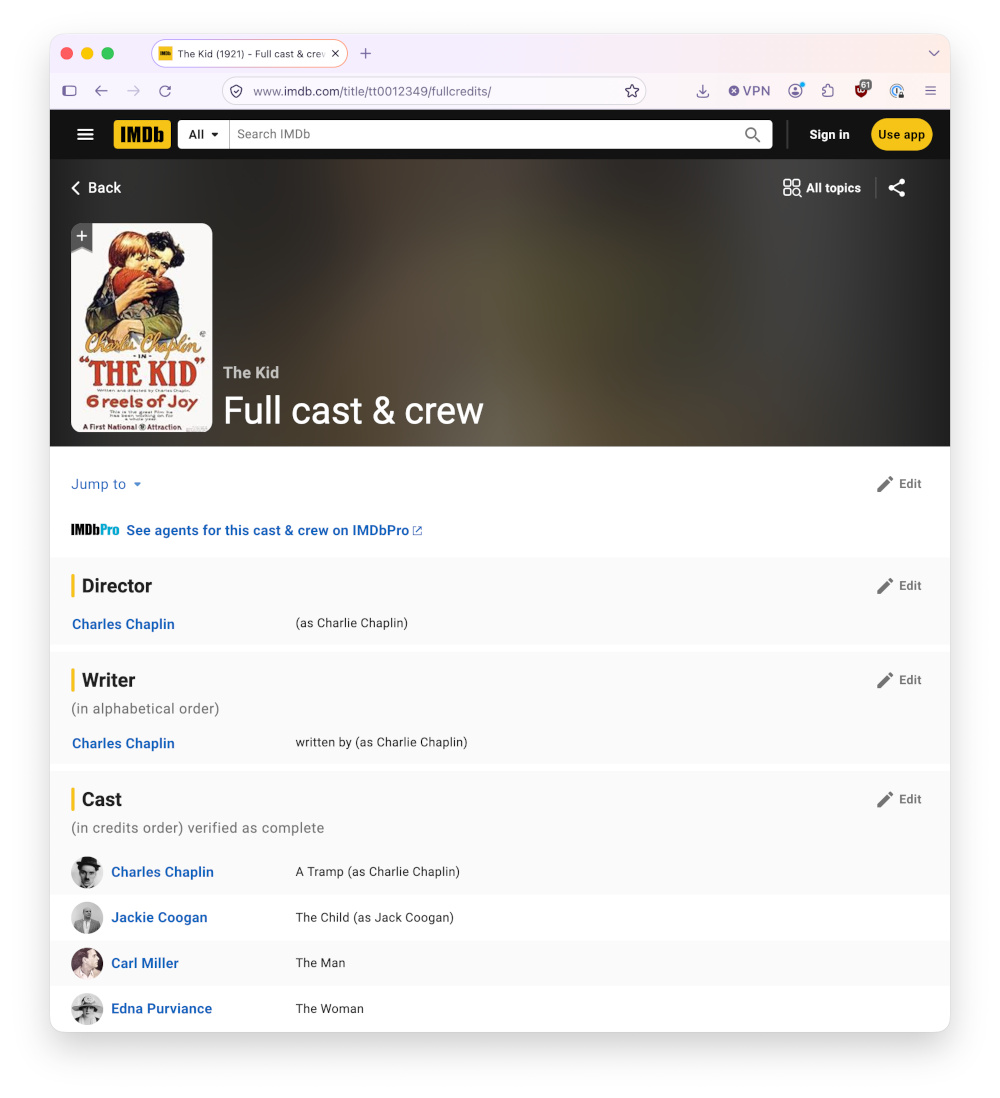
\includegraphics[height=\paperheight]{images/the-kid.jpg}};
    \end{tikzpicture}
\end{frame}
\inlineslide{s:the-kid-imdb}{}\label{l:the-kid-imdb}

\againframe{moviedb-kid1}
\againframe{moviedb-kid2}

In this lecture we look at a different way of representing the same data: as \emph{documents}, each of which holds everything about one movie, or one person, in a single nested structure.
Documents are usually encoded as JSON (XML was used for this purpose in the past, but it has fallen out of favour).
JSON is also the most common format for exchanging data between web browsers/mobile apps and servers.
Using the same format in the database as for web APIs can reduce the amount of code required to convert between different representations.

On the course web page you will find a version of the movies database that contains (more or less) the same information as the relational database we have studied so far, but represented as JSON documents instead.
There are some databases that specialise in JSON documents as their data model, but we will use the same DBMS (DuckDB) for the document data as for the relational data, since it has good built-in support for JSON data.
That means we will be able to query that JSON data using SQL, and we will use that example database to discuss the trade-offs between the relational and the document representation.

\subsection{JSON documents}\label{sec:json-documents}

JSON, short for \emph{JavaScript Object Notation}, began as the subset of the JavaScript language used for writing down data values, and is now a standard of its own \citep{RFC8259}.
A JSON value is one of the following: a string in double quotes; a number; one of the literals \code{true}, \code{false}, and \code{null}; an \emph{array}, which is an ordered list of values in square brackets; or an \emph{object}, which is a set of key-value pairs in curly braces, where every key is a string.
The values in an array or object can be any JSON values, including other arrays and objects, so they can be nested to any depth.

\begin{frame}
    \label{s:json-syntax}
    \frametitle{JSON: JavaScript Object Notation}
    \inputminted[fontsize=\footnotesize]{json}{code/json-example.json}
    \vspace{0.5em}
    \begin{itemize}
        \item \textbf{Object}: key-value pairs in \code{{...}}; keys are strings
        \item \textbf{Array}: ordered list of values in \code{[...]}
        \item \textbf{Scalars}: string, number, \code{true}, \code{false}, \code{null}\\[1em]\pause
    \end{itemize}
    Objects and arrays nest to any depth: a JSON value is a \textbf{tree}\\[1em]
    Used everywhere: web APIs, configuration files, logs, \dots\\
    Every programming language can read and write it
\end{frame}
\inlineslide{s:json-syntax}{}\label{l:json-syntax}

Despite its name, JSON is not tied to JavaScript: virtually every programming language has a library for reading and writing it.
A JSON object corresponds naturally to a dictionary in Python or a map in Java, and an array to a list.
JSON's datatypes are quite minimal: for example, there is only one type of number, which does not distinguish between integers and floating-point numbers, and there is no type for dates and times (they are typically represented as strings).

A \emph{document} is a JSON object that is stored as one unit in a database, usually with a unique identifier that serves as a primary key.
\autoref{l:json-movie} shows the document for \emph{The Kid} in the JSON version of our example database.
It has been abridged to fit on the slide: the comments \code{/* ... */} mark where some elements or keys have been left out, and are not part of the document (JSON does not actually allow comments).

\begin{frame}
    \label{s:json-movie}
    \frametitle{A movie as a JSON document}
    {\scriptsize% The Kid's document in the movies table, abridged, for s:json-movie
% Generated from json-kid-doc.sql by examples/render.py -- do not edit.
% Regenerate with: make examples
\inputminted{json}{examples/json-kid-doc.json}%
}
\end{frame}
\inlineslide{s:json-movie}{}\label{l:json-movie}

The top-level keys \code{movie_id}, \code{title}, \code{year}, \code{type}, and \code{minutes} hold the same values as the corresponding columns of the \code{movies} table, and \code{rating} and \code{rating_votes} hold the values from the \code{ratings} table.
Everything else is nested.
The genres are an array of strings, so the movie carries its own genre names and there is no need for a separate \code{has_genre} table.
The cast is an array of objects under the \code{actors} key, with one object per actor containing the actor's ID, their name, and an array of the characters they played.
The \code{directors}, \code{producers}, \code{writers}, and \code{composers} arrays (left out on the slide) are similar, but with a \code{job} key in place of \code{roles}.
Finally, \code{trivia_entries} is an array of strings, each a snippet of trivia about the movie taken from the IMDb website.
These exist only in the JSON version of the database, not in the relational one.

People are documents too, stored separately from the movies, as shown on \autoref{l:json-person}.
A person's document contains their own details, plus an array for each type of position they have held: \code{acted_in}, \code{directed}, \code{produced}, \code{wrote}, and \code{composed_for}.
Each element of these arrays describes one movie, with its ID, title, and year, plus either the roles played or the job.

\begin{frame}
    \label{s:json-person}
    \frametitle{A person as a JSON document}
    {\scriptsize% Charles Chaplin's document in the people table, abridged, for s:json-person
% Generated from json-chaplin-doc.sql by examples/render.py -- do not edit.
% Regenerate with: make examples
\inputminted{json}{examples/json-chaplin-doc.json}%
}
\end{frame}
\inlineslide{s:json-person}{}\label{l:json-person}

Each of these arrays is present only if the person actually held that type of position, so a person who has never acted has no \code{acted_in} key.
Alfred Hitchcock's document, for example, has only the keys % The keys of Alfred Hitchcock's document, for the prose after s:json-person
% Generated from json-hitchcock-keys.sql by examples/render.py -- do not edit.
% Regenerate with: make examples
\texttt{person\_id}, \texttt{name}, \texttt{birthyear}, \texttt{deathyear}, and \texttt{directed}%
.
In the same way, \code{birthyear} or \code{deathyear} is omitted when it is unknown, rather than being set to \code{null}.
Elements of the same array need not have the same keys either: across all the people documents, \jsondirectedjob\ elements of \code{directed} arrays have a \code{job} key and \jsondirectednojob\ do not.
There is nothing forcing two documents, or two elements of one array, to have the same structure.

\autoref{l:json-structure} summarises the structure of both types of document.
Notice that the many-to-many relationship between movies and people, which the relational schema represents with the \code{has_position} and \code{plays_role} tables, now appears twice: once inside each movie document (in the \code{actors}, \code{directors}, \dots\ arrays), and once inside each person document (in \code{acted_in}, \code{directed}, \dots).
In both directions, the nested objects contain the ID of the document they refer to, plus a copy of some of its fields~-- the person's name, or the movie's title and year~-- so that each document is useful on its own, without having to look up the other.

\begin{frame}
    \label{s:json-structure}
    \frametitle{The structure of the documents}
    % Schema-level only: key names, no values, so it is hard-coded rather than generated.
    % Each document is an outer box with a header band; an array of objects is a nested box
    % listing the keys of its elements. The two references by ID are routed through the
    % gap between the documents, which forces one crossing: each starts low in one document
    % and ends high in the other. Each document's own key is underlined, as on s:moviedb-schema.
    \begin{center}
    \begin{tikzpicture}[font=\scriptsize]
        \tikzstyle{key}=[anchor=west,font=\scriptsize\ttfamily,inner sep=1pt]
        \tikzstyle{nested}=[draw,fill=blue!8,rounded corners=2pt]
        \tikzstyle{ref}=[-{Stealth[length=2.2mm]},thick]
        % The movie document
        \draw [thick,fill=red!8] (0,0.6) rectangle (4.6,6.0);
        \draw [thick,fill=red!30] (0,5.5) rectangle (4.6,6.0);
        \node [anchor=west] at (0.1,5.75) {\textbf{movies}: one per movie};
        \node [key] (mid) at (0.15,5.25) {\underline{movie\_id}};
        \node [key] at (0.15,4.87) {title, year, type, minutes};
        \node [key] at (0.15,4.49) {rating, rating\_votes};
        \node [key] at (0.15,4.11) {genres: [string, \dots]};
        \node [key] at (0.15,3.73) {actors: [};
        \draw [nested] (0.4,2.7) rectangle (4.4,3.5);
        \node [key] at (0.5,3.3) {name, roles: [\dots]};
        \node [key,anchor=east] (pa) at (4.3,2.92) {person\_id};
        \node [key] at (0.15,2.45) {directors, producers,};
        \node [key] at (0.15,2.07) {writers, composers: [};
        \draw [nested] (0.4,1.4) rectangle (4.4,1.85);
        \node [key] (pb) at (0.5,1.62) {name, job, person\_id};
        \node [key] at (0.15,1.0) {trivia\_entries: [string, \dots]};
        % The person document
        \draw [thick,fill=red!8] (5.9,1.85) rectangle (10.6,6.0);
        \draw [thick,fill=red!30] (5.9,5.5) rectangle (10.6,6.0);
        \node [anchor=west] at (6.0,5.75) {\textbf{people}: one per person};
        \node [key] (pid) at (6.05,5.25) {\underline{person\_id}};
        \node [key] at (6.05,4.87) {name, birthyear, deathyear};
        \node [key] at (6.05,4.49) {acted\_in: [};
        \draw [nested] (6.2,3.47) rectangle (10.4,4.27);
        \node [key] (ma) at (6.3,4.07) {movie\_id};
        \node [key] at (6.3,3.69) {title, year, roles: [\dots]};
        \node [key] at (6.05,3.22) {directed, produced,};
        \node [key] at (6.05,2.84) {wrote, composed\_for: [};
        \draw [nested] (6.2,2.17) rectangle (10.4,2.62);
        \node [key] (mb) at (6.3,2.39) {movie\_id, title, year, job};
        % References by ID, through the gap between the documents
        \draw<2-> [ref] (pa.east) -- (5.05,2.92) -- (5.05,5.25) -- (5.9,5.25);
        \draw<2-> [ref] (pb.east) -- (5.05,1.62) -- (5.05,2.92);
        \draw<2-> [ref] (ma.west) -- (5.45,4.07) -- (5.45,5.75) -- (4.6,5.75);
        \draw<2-> [ref] (mb.west) -- (5.45,2.39) -- (5.45,4.07);
    \end{tikzpicture}
    \end{center}
    \uncover<2->{Arrows: references by ID.
    Names and titles are also \textbf{copied}.}\\[0.3em]%
    \uncover<3->{Each movie--person relationship is stored twice, once in each direction.}
\end{frame}
\inlineslide{s:json-structure}{}\label{l:json-structure}

To store these documents in DuckDB, we will use its \code{JSON} data type.
The JSON version of the example database consists of the two tables on \autoref{l:json-tables}, each with one row per document.
Each table has a primary key column holding the same ID as in the relational database, and a column of type \code{JSON} holding the document itself, named \code{movie} or \code{person} after what the document describes.
As far as the database is concerned, that column contains arbitrary JSON: the database imposes no further structure on the documents, and the constraints we discussed in \autoref{sec:relational} do not apply.
The database is available as a separate file on the course web page, and you can open it in the same way as the relational one.

\begin{frame}
    \label{s:json-tables}
    \frametitle{Documents in DuckDB}
    \inputminted[fontsize=\footnotesize]{sql}{code/json-tables.sql}
    \vspace{0.6em}
    One row per document: \jsonmovies\ movies, \jsonpeople\ people\\[0.5em]
    Everything except the ID is inside the documents\\[0.5em]
    The database knows nothing about the structure of the documents\\[0.5em]
    Download it from the course web page
\end{frame}
\inlineslide{s:json-tables}{}\label{l:json-tables}

Our two-column tables imitate a \emph{document database}, which is a type of database built around storing documents.
MongoDB is the best-known example; others include CouchDB and Couchbase.
A document database stores \emph{collections} of documents (MongoDB's term for what is essentially a table), and each document has a unique key (called \code{_id} in MongoDB).
Documents in a collection do not have to have the same structure, and by default the database does not enforce any schema (though some document databases can optionally enforce one, as we will see on \autoref{l:json-schema}).

Document databases sometimes have their own query languages instead of SQL.
\autoref{l:document-databases} shows some queries in MongoDB's query language, in which the filter is itself written as a JSON-like object describing the documents that should match.
The second query shows a convenient feature of this language: a condition on a key whose value is an array, like \code{genres}, matches if any element of the array satisfies it.
The third reaches into the objects nested inside the \code{directors} array using a dotted path.

\begin{frame}
    \label{s:document-databases}
    \frametitle{Document databases}
    \textbf{Document databases}: e.g.\ MongoDB, CouchDB
    \begin{itemize}
        \item Store \textbf{collections} of documents, each with a key
        \item No fixed schema; own query languages\\[0.5em]
    \end{itemize}
    MongoDB queries:
    \inputminted[fontsize=\footnotesize]{javascript}{code/mongodb-find.js}
    \vspace{0.5em}\pause
    \textbf{Relational databases} have added JSON support too:
    \begin{itemize}
        \item PostgreSQL, MySQL, SQLite, DuckDB, \dots
        \item JSON functions in the SQL standard since 2016
    \end{itemize}
\end{frame}
\inlineslide{s:document-databases}{}\label{l:document-databases}

Meanwhile, most relational databases have added support for storing and querying JSON, and the SQL standard has included functions for working with JSON since 2016.
So you don't necessarily have to choose between a relational and a document database, but you can combine both approaches to data modelling in a single database that uses both relational and document elements as appropriate.
We will see how to query documents with SQL in \autoref{sec:json-sql}.

\subsection{Normalisation and denormalisation}\label{sec:normalisation}

\begin{frame}
    \label{s:redundancy}
    \frametitle{Redundancy}
    \textbf{Relational:} Charles Chaplin's name is stored once\\
    (in a row of \code{people}; other tables refer to \code{nm0000122})\\[1em]\pause
    \textbf{Documents:} his name is stored
    \begin{itemize}
        \item once in his own document in \code{people}
        \item \jsonchaplinmentions\ times in \jsonchaplindocs\ movie documents\\
            (once per credit: in \code{actors}, \code{directors}, \dots)\\[0.5em]
    \end{itemize}
    The title of \emph{The Kid}: in its own document, and in \jsonkiddocs\ people documents\\[1em]\pause
    \textbf{Redundancy}: the same fact is stored in several places
\end{frame}
\inlineslide{s:redundancy}{}\label{l:redundancy}

Storing the same piece of information in several places is called \emph{redundancy}.
A schema that avoids redundancy, so that every fact is stored in exactly one place and everything else refers to it by its key, is called \emph{normalised}.
A schema that deliberately stores copies of data in the places where they are needed is called \emph{denormalised}.
Our relational schema is normalised, and our document schema is denormalised.

The question of normalisation vs.\ denormalisation is not specific to documents.
A relational schema can be denormalised too: for example, if we added a \code{title} column to \code{plays_role}, so that the cast of a movie could be listed together with the movie's title without joining with \code{movies}, the titles would be stored redundantly.
Conversely, documents can be normalised: if the movie documents contained only the IDs of their actors, and not their names, then each name would be stored in only one place, but then we would need a join to find the actors' names.

\begin{frame}
    \label{s:normalisation}
    \frametitle{Normalised and denormalised data}
    \textbf{Normalised}: every fact is stored in exactly one place
    \begin{itemize}
        \item Other places refer to it by its key
        \item The key is an ID that never needs to change
        \item Reading often requires joins to look up referenced data\\[1em]\pause
    \end{itemize}
    \textbf{Denormalised}: copies of facts are stored where they are needed for reads
    \begin{itemize}
        \item Reads are faster and simpler: fewer joins
        \item Writes are slower and more complex: all copies must be updated
        \item Copies may become inconsistent with each other\\[1em]\pause
    \end{itemize}
    \textbf{Relational} DBs: often normalised, can be denormalised\\
    \textbf{Document} DBs: often denormalised, can be normalised
\end{frame}
\inlineslide{s:normalisation}{}\label{l:normalisation}

The trouble with redundancy comes when the data changes.
Suppose a person changes their name, as the film director Lana Wachowski did: every credit on her movies should then show her current name.
In the relational database, as shown on \autoref{l:update-anomaly}, this is a single \code{UPDATE} of one row.
In the document database, the application has to update the person's document, and then find and update every movie document that contains a copy of the name.
It's more expensive to find and update all of these copies.
Moreover, if you accidentally miss one, or the application crashes halfway through making the updates, the copies of the name may become inconsistent with each other.
This is known as an \emph{update anomaly}, and there is nothing in the database to prevent it.

\begin{frame}
    \label{s:update-anomaly}
    \frametitle{Updating denormalised data}
    If someone changed their name:\\[0.8em]
    \textbf{Relational:} change one row
    \inputminted[fontsize=\footnotesize]{sql}{code/rename-relational.sql}
    \vspace{0.8em}\pause
    \textbf{Documents:} change the person's document, \textbf{and} every movie document containing a copy of the name
    \begin{itemize}
        \item Application must find all the copies
        \item Missed one $\Rightarrow$ copies disagree
        \item Crashed halfway $\Rightarrow$ copies disagree\\[0.8em]
    \end{itemize}
    This is an \textbf{update anomaly}
\end{frame}
\inlineslide{s:update-anomaly}{}\label{l:update-anomaly}

Redundancy can also cause other problems.
In the document database, the genre names exist only inside the movie documents.
If we deleted the last movie in a particular genre, the genre would vanish from the database entirely; this is known as a \emph{deletion anomaly}.
And it is impossible to record a new genre until there is a movie that has it; this is called an \emph{insertion anomaly}.
The relational schema, with its separate \code{genres} table, has neither problem.

The relational model makes the avoidance of redundancy a formal part of its theory, through a series of \emph{normal forms}.
The first of these, \emph{first normal form} (1NF), requires every value in a table to be atomic: that is, a single number or string, not a list or a nested record.
This is why the relational schema needs the \code{has_genre} table: in first normal form, a movie's genres cannot be stored as a list in a column of the \code{movies} table, so we have one row per pairing of a movie and a genre instead.
Documents violate first normal form by design.

The further normal forms (second and third normal form, Boyce--Codd normal form, and others) remove other kinds of redundancy, for example where one column's value is determined by another column that is not the table's key \citep{Kent1983}.
We will not go into their formal definitions in this course; the principle that each fact should be stored in one place is the important idea.

\begin{frame}
    \label{s:normal-forms}
    \frametitle{Normal forms}
    \textbf{First normal form} (1NF): every value in a table is \textbf{atomic}\\
    (a single number or string, not a list or nested record)\\[1em]
    \textbf{Relational}: one row per movie--genre pair in \code{has_genre}\\[0.3em]
    \textbf{Document}: \mintinline{json}{"genres": ["Comedy", "Drama"]}\\
    \hspace*{1em}$\Rightarrow$ violates 1NF\\[1em]\pause
    Further normal forms (2NF, 3NF, BCNF, \dots)
    remove other kinds of redundancy\\[1em]\pause
    \textbf{You can choose to intentionally violate normal forms}:\\
    Many databases support JSON and list/array types
\end{frame}
\inlineslide{s:normal-forms}{}\label{l:normal-forms}

If redundancy causes so many problems, why would anyone denormalise?
The answer is that it makes reads faster and simpler.
To show a web page about a movie, an application using the document database reads one document, while an application using the relational database needs to query most of the seven tables.
In the document model, data that is read together is stored together, a property called \emph{locality}, which matters especially when the data is on disk or on another machine, where each separate lookup has a cost.
Denormalisation is common in relational databases too: for example, a discussion forum may store the number of replies in each thread's row, rather than counting the replies every time it displays the list of threads.

The trade-off is that denormalisation makes reads faster at the cost of making writes slower and more error-prone.
A useful way of thinking about this is that the normalised data is the authoritative version of the data, or the \emph{source of truth}, and the denormalised data is \emph{derived} from it.
If the derived data is ever lost or corrupted, it can be regenerated from the source of truth.

\begin{frame}
    \label{s:why-denormalise}
    \frametitle{Why denormalise?}
    To make \textbf{reads} fast and simple:
    \begin{itemize}
        \item Movie web page: read one document, no joins
        \item Data that is read together is stored together (\textbf{locality})
        \item Precompute expensive results, e.g.\ counts\\[1em]\pause
    \end{itemize}
    At the cost of making \textbf{writes} slower and more complex:
    \begin{itemize}
        \item More data to write and store
        \item Application must keep all copies consistent\\[1em]\pause
    \end{itemize}
    Normalised data is \textbf{source of truth};\\
    denormalised data is \textbf{derived} from it.\\[0.5em]
    Best if you can regenerate the denormalised data anytime.
\end{frame}
\inlineslide{s:why-denormalise}{}\label{l:why-denormalise}

\supervision{\label{q:index-redundancy}
    An index, which we discussed in the introduction, is also a form of redundancy: the values of the indexed column are stored both in the table and in the index.
    In what ways is an index similar to denormalisation, and in what ways is it different?
    Consider who is responsible for keeping the copies consistent, what happens on reads and on writes, and whether the choice affects how queries are written and what they return.
}{
    Similarities:
    \begin{itemize}
        \item Both store a redundant copy of some data, arranged so that a particular kind of read is fast: an index on \code{year} makes it fast to find the movies from a given year, just as an \code{acted_in} array makes it fast to find the movies of a given person.
        \item Both trade write performance and storage space for read performance: every insert, update, or delete must also update the index, just as it must update every copy of denormalised data.
        \item Both are derived data: the table is the source of truth, and an index can be dropped and rebuilt from it at any time, just as denormalised values can be regenerated from normalised data.
        \item Both have to be chosen with knowledge of the queries that will be run: neither helps a query that it was not designed for.
    \end{itemize}
    Differences:
    \begin{itemize}
        \item An index is maintained by the database, automatically and within the same transaction as the write that changed the table.
            It therefore can't become inconsistent with the table, and there are no update anomalies.
            Denormalised copies are typically maintained by the application, which has to find and update every copy, and may get it wrong.
        \item An index belongs to the physical representation of the data, not the logical one (it is an example of data independence).
            Queries are written against the tables, and return the same results whether or not an index exists; the query optimiser decides whether to use it.
            Denormalisation changes the logical schema: queries have to be written to read from the denormalised copy, and if the copy is wrong, so is the result.
        \item An index usually stores only the indexed values and a reference to the row they came from, so a lookup typically still needs to read the row itself.
            Denormalised data usually copies whole fields, so that the read needs nothing else.
        \item An index is built from a single table, whereas denormalisation often combines data from several tables, in effect storing the result of a join, as the movie documents do with the names of the actors.
    \end{itemize}
    So an index gives some of the read performance benefits of denormalisation without the consistency risks, because the database takes on the job of keeping the copies in sync.
    Some databases go further and offer \emph{materialised views}, which store the result of an arbitrary query (including joins) and keep it up to date as the underlying tables change, either automatically or when explicitly refreshed.
    These are, in effect, denormalisation that is managed by the database rather than by the application.
}

\supervision{\label{q:json-build}
    Write a SQL query over the relational version of the example database that produces one JSON document per movie, containing the movie's ID, title, and year, its genres as an array of strings, and its actors as an array of objects, each with the actor's \code{person_id} and \code{name}.
    You will need DuckDB's \code{json_object} function, which takes alternating keys and values and returns a JSON object, and the \code{list} aggregate function, which collects the values in a group into a list.
    How does your output differ from the documents in the JSON version of the database?
}{
    Each array is the result of a correlated subquery that aggregates the rows for one movie into a list:
    \inputminted[fontsize=\small]{sql}{code/q-json-build.sql}
    For \emph{The Kid}, this produces (abridged):
    \begin{quote}% The document code/q-json-build.sql builds for The Kid, for the solution to q:json-build
% Generated from q-json-build.sql by examples/render.py -- do not edit.
% Regenerate with: make examples
\inputminted{json}{examples/q-json-build.json}%
\end{quote}
    Some differences from the documents in the JSON database:
    \begin{itemize}
        \item The JSON database lists each movie's actors in the order in which IMDb lists them.
            The relational schema has no column recording this order, so it cannot be reproduced; the query returns the actors in an arbitrary order.
            Arrays are ordered, whereas the rows of a table are not.
        \item A movie with no actors gets a \code{null} under \code{actors} (since the aggregate over zero rows is null), whereas the JSON database leaves out the key.
            You could fix this using \code{coalesce} to substitute an empty list, or by building the object in a way that omits the key.
        \item The genres are sorted alphabetically, because of the \code{ORDER BY} inside the \code{list} aggregate.
            Without it, their order would be arbitrary, for the same reason as the actors'.
    \end{itemize}
    The other arrays (\code{directors}, \code{producers}, \dots, and the \code{roles} of each actor, which come from \code{plays_role}) can be added in the same way.
    The query to build the people documents is similar, with the subqueries going from people to movies instead.
}


\subsection{Comparing the relational and document models}\label{sec:document-tradeoffs}

The JSON documents and the relational tables contain the same information (apart from the trivia), so which representation is better?
As usual, it depends on how the data is used.

Documents work best for data that has the shape of a tree: an entity, with things nested inside it that belong to that entity and nothing else.
A movie's trivia entries are an example: each entry is about one movie, and it makes sense to store it with that movie, in a one-to-many relationship between the movie and its trivia entries.
A one-to-one relationship, such as that between a movie and its rating, is easy to represent too: the related fields can simply be stored as keys within the document, as \code{rating} and \code{rating_votes} are.
In a relational schema, one-to-many relationships need a separate table, and reading an entity with its details needs a join.

\begin{frame}
    \label{s:document-relationships}
    \frametitle{Representing relationships as documents}
    \textbf{One-to-one}: keys in the same document\\
    (\code{rating}, \code{rating_votes})\\[0.8em]\pause
    \textbf{One-to-many}: an array nested inside the document\\
    (\code{trivia_entries}: each entry belongs to one movie)\\[0.8em]
    Document is a \textbf{tree}: a good fit\\[0.8em]\pause
    \textbf{Many-to-many}: not a tree.
    \begin{itemize}
        \item Can store array of IDs, but needs a join on read
        \item Want to query in both directions?\\
            (All of a movie's cast, all movies an actor has played in)\\
            $\Rightarrow$ store the relationship twice, or use a secondary index\\[0.8em]
    \end{itemize}
    Document model is awkward for many-to-many relationships.
\end{frame}
\inlineslide{s:document-relationships}{}\label{l:document-relationships}

Many-to-many relationships, like that between movies and people, are more awkward to represent as documents.
A movie has many people, and a person works on many movies, so the data is not a tree but a graph, and there is no single document that naturally contains both.
As we have seen, our example database stores each such relationship twice, with duplicated data, so that both movies and people are self-contained, and accepts the costs of denormalisation in exchange.
The alternative is to store only IDs, and to look up the referenced documents when reading, which is essentially a join.
Since document databases are designed for self-contained documents, some of them don't support joins on queries, leaving the application to perform the join itself by individually fetching each referenced document, like in the index nested loop join on \autoref{l:join-algorithms}.

Another difference is how the structure of the data is defined.
A relational database has a schema that is enforced on every write: you cannot insert a row with a column that the table doesn't have, or a string into an integer column.
This is sometimes called \emph{schema-on-write}.
A document database usually accepts any JSON document.
This is sometimes called ``schemaless'', but that is misleading: the code that reads the documents assumes that they have a certain structure, such as a \code{name} key whose value is a string.
There is still a schema, but it is implicit, and only checked when the data is read, which is why it is better called \emph{schema-on-read} \citep{Kleppmann2026}.
This is analogous to the difference between static type checking in languages like Java and OCaml, where the compiler checks types before the program runs, and dynamic type checking in languages like Python, where errors due to type mismatches surface only at runtime.

\begin{frame}
    \label{s:schema-on-read}
    \frametitle{Schema-on-write and schema-on-read}
    \textbf{Schema-on-write} (relational): database checks every write against the schema\\[0.5em]
    Advantage: reads return known types; can type-check queries\\[1em]
    \textbf{Schema-on-read} (documents): any JSON is accepted on write, but the code reading it assumes a structure\\[0.5em]\pause
    Advantages:
    \begin{itemize}
        \item \textbf{Heterogeneous data} with many different types of rows in the same table
            \begin{itemize}
                \item e.g.\ products in an online shop: books, shoes, or TVs have different attributes\\[0.5em]\pause
            \end{itemize}
        \item \textbf{Schema changes}: allow database to contain a mixture of old and new formats, support both on read
            \begin{itemize}
                \item Avoids an expensive schema migration
            \end{itemize}
    \end{itemize}
\end{frame}
\inlineslide{s:schema-on-read}{}\label{l:schema-on-read}

Schema migrations in a relational database (\autoref{l:ddl-alter}) can be expensive: for example, adding a new column, filling it in for every existing row, and dropping the old column can be slow for a large table.
With documents, we can simply start writing new documents in the new format, and have the application handle both formats when reading.
Schema-on-read is also convenient when the items in a collection inherently have different structures, and creating a separate table for every type of item would be impractical.

The downside of schema-on-read is that mistakes are not caught.
Nothing stops one part of an application from writing \code{birthyear}, another \code{birthYear}, and a third \code{birth_year}, or from storing a year as the string \code{"1889"} rather than the number \code{1889}.
And a query with a misspelt key does not produce an error: looking up a key that a document doesn't have simply returns null.

\supervision{\label{q:doc-or-relational}
    For each of the following applications, would you store the data in a relational schema or as documents?
    Justify your answers, and if you choose documents, say what each document would contain.
    \begin{enumerate}
        \item A blogging platform, where each post has a title, a body text, some tags, and comments from readers.
        \item A bank, which stores customers, their accounts, and the transfers between accounts.
        \item An event log, which stores every time various functions were invoked, and what arguments were passed to the function invocation.
        \item An online shop's product catalogue, in which different types of product have different attributes.
        \item A system for storing the settings of a mobile app, such as the user's preferred language, notification preferences, and so on.
    \end{enumerate}
}{
    There is not one right answer to any of these; a good answer identifies the access patterns and relationships, and weighs the trade-offs.
    \begin{enumerate}
        \item A post with its tags and comments is a natural tree, and is typically read as a whole when the post is displayed, so a document per post works well, with an array of tags and an array of comments.
            However, each comment has an author, who is a user of the platform: if the post embeds the author's display name in each comment, changing that name requires updating every post the user has commented on.
            Storing only the user ID in the comment avoids this, at the cost of a join when displaying the post.
            If the number of comments can be very large, embedding all of them in the post document makes the document grow without bound, and it may be better to store comments separately.
            A relational schema (posts, tags, post--tag join table, comments, users) is also perfectly reasonable.
        \item Relational.
            Transfers relate two accounts, each account may belong to several customers and each customer may have several accounts, so the data has many-to-many relationships.
            A transfer must update two account balances atomically, and the bank needs strong integrity constraints (every transfer refers to accounts that exist, balances are numbers, \dots), which a relational database enforces with a schema, foreign keys, and transactions.
            Embedding transfers in account documents would store each transfer twice (in the sending and the receiving account), with the risk of the two copies disagreeing.
        \item If there are many different functions, then documents are the best fit, because each function may have different arguments.
            Storing invocations in a relational schema would require either a separate table for each function (impractical if there are more than, say, a dozen), or a table that has a column for any of the arguments that might be passed to any of the functions (most of which would have to be null for a given invocation).
            A third possible relational representation would be a table of \code{(invocation_id, argument_name, argument_value)} triples, which is awkward to query, inefficient (requiring lots of rows), and cannot enforce that the value of an argument has the type expected for its name.
            In JSON this data is much easier to represent.
        \item The settings of one user can be conveniently represented as a tree, and since it's a small amount of data, it can be read and written as a whole.
            Moreover, there's no relationship between one user's settings and another user's settings, so a document per user is a good fit.
            New settings are added with each version of the app, which is easy with schema-on-read: the app supplies a default for any key that is missing.
    \end{enumerate}
}

\emph{JSON Schema} \citep{JSONSchema2022,Pezoa2016} is a widely used language for defining what structure a JSON document is supposed to have.
A JSON Schema is itself a JSON document.
A \emph{validator} is a program that takes a schema and a JSON value, and reports whether the value is valid according to the schema (and if not, what is wrong with it).
Validators exist for many programming languages, and some databases also support validating JSON documents against a schema on write.
JSON Schema is widely used to describe the data exchanged between systems, for example in the OpenAPI format for documenting web APIs, and tools can generate documentation, code, and input forms from a schema.

\autoref{l:json-schema} shows part of a JSON Schema for the people documents in our example database.
The \code{type} keyword says what type of JSON value is allowed (\code{object}, \code{array}, \code{string}, \code{integer}, and so on).
For an object, \code{properties} specifies a schema for the value of each key, \code{required} lists the keys that must be present, and \code{additionalProperties: false} means that no other keys besides those listed in the schema are allowed.
For an array, \code{items} specifies the schema that every element must satisfy, and for a string, you can enforce that each value must match some regular expression using \code{pattern}.
Note that the schema allows \code{birthyear} and \code{deathyear} to be absent, which is how our documents represent an unknown value, but if they are present, they must be integers.

\begin{frame}
    \label{s:json-schema}
    \frametitle{JSON Schema for people documents}
    \inputminted[fontsize=\scriptsize]{json}{code/person-schema.json}
\end{frame}
\inlineslide{s:json-schema}{}\label{l:json-schema}

\supervision{\label{q:json-schema-limits}
    Which of the following properties of the people documents in the example database can be enforced by a JSON Schema, and which cannot?
    Explain why.
    \begin{enumerate}
        \item Every person has a name.
        \item A person's \code{deathyear}, if present, is not earlier than their \code{birthyear}.
        \item No two documents have the same \code{person_id}.
        \item Every \code{movie_id} in a person's \code{acted_in} array is the ID of a movie document.
        \item The \code{title} in each element of \code{acted_in} is the same as the title in the corresponding movie document.
    \end{enumerate}
}{
    \begin{enumerate}
        \item Yes: \code{"required": ["person_id", "name"]}, together with \code{"type": "string"} for the \code{name} property.
        \item No, at least not with the keywords covered in the notes: JSON Schema constrains each value separately (its type, range, pattern, and so on), and has no way of comparing the values of two keys in the same document.
            (This would be easy as a \code{CHECK} constraint in SQL.)
        \item No: a JSON Schema validates one document at a time, and uniqueness is a property of the whole collection.
            In our DuckDB tables, this could be enforced by the primary key on the \code{person_id} column, together with a \code{CHECK} constraint ensuring that the key column agrees with the ID inside the document.
        \item No: this is referential integrity, which depends on the contents of a different collection.
            In the relational database it is a foreign key constraint.
            In a document database, the application has to ensure it.
        \item No, for the same reason: it is a relationship between two documents.
            This is exactly the consistency between redundant copies that is problematic in a denormalised database.
    \end{enumerate}
    In general, a JSON Schema can describe the structure of an individual document, but not any constraint involving several documents.
    Those are the constraints that a relational database expresses with primary keys, foreign keys, and normalisation.
}


\subsection{Querying JSON in SQL}\label{sec:json-sql}

To look inside a JSON document in SQL, DuckDB provides two operators, \code{->} and \code{->>}, which are equivalent to the functions \code{json_extract} and \code{json_extract_string} respectively.

\begin{frame}
    \label{s:json-arrows}
    \frametitle{Extracting values: \code{->} and \code{->>}}
    \inputminted[fontsize=\footnotesize]{sql}{code/json-arrows.sql}
    \vspace{0.3em}
    {\footnotesize% Result of the arrow-operator example on s:json-arrows
% Generated from json-arrows.sql by examples/render.py -- do not edit.
% Regenerate with: make examples
\begin{tabular}{|l|l|l|}\hline
    \textbf{title\_json} & \textbf{title\_text} & \textbf{genres} \\\hline
    \texttt{"The Kid"} & The Kid & \texttt{["Comedy","Drama","Family"]} \\\hline
\end{tabular}%
}\\[1em]
    \code{->} returns a value of the \textbf{JSON} type (note the quotes)\\
    \code{->>} returns a \textbf{SQL string} (\code{VARCHAR})\\[1em]\pause
    Not standard SQL: other databases have different syntax\\
    (PostgreSQL uses the same operators)
\end{frame}
\inlineslide{s:json-arrows}{}\label{l:json-arrows}

The right-hand side of the arrow can be a key, as in \code{movie->'title'}, or a \emph{JSONPath} expression, which can reach deeper inside the document, as shown on \autoref{l:json-path}.
A JSONPath expression starts with \code{$}, which stands for the whole document, and is followed by a series of steps: \code{.actors} selects the value of the \code{actors} key, and \code{[0]} selects the first element of an array.
(JSON arrays are indexed from zero, whereas DuckDB's own lists are indexed from one.)
The wildcard \code{[*]} selects every element of an array, and so a path containing it returns not a single value, but a list of values.
DuckDB represents this as a value of type \code{VARCHAR[]} (a list of strings) for \code{->>}, or a list of JSON values for \code{->}.

\begin{frame}
    \label{s:json-path}
    \frametitle{JSONPath: reaching inside a document}
    \inputminted[fontsize=\footnotesize]{sql}{code/json-path.sql}
    \vspace{0.3em}
    {\footnotesize% Result of the JSONPath example on s:json-path
% Generated from json-path.sql by examples/render.py -- do not edit.
% Regenerate with: make examples
\begin{tabular}{|l|l|l|}\hline
    \textbf{first\_actor} & \textbf{second\_genre} & \textbf{all\_genres} \\\hline
    Charles Chaplin & Drama & [Comedy, Drama, Family] \\\hline
\end{tabular}%
}\\[1em]
    \begin{tabular}{@{}l@{\hspace{1em}}l@{}}
        \code{$} & the whole document \\
        \code{.actors} & value of the key \code{actors} \\
        \code{[0]} & first element of an array (counting from 0) \\
        \code{[*]} & every element of an array $\Rightarrow$ result is a \textbf{list}
    \end{tabular}
\end{frame}
\inlineslide{s:json-path}{}\label{l:json-path}

With these operators we can use the values inside documents in a \code{WHERE} clause, to perform selection, and in a \code{SELECT} clause, to perform projection.
There are two things to watch out for.

First, \code{->>} returns a string, even when the value in the document is a number.
To compare a number with a number, rather than a string with a string, we must convert it with a \emph{cast}.
The standard SQL syntax for this is \code{CAST(x AS INTEGER)}, and DuckDB also accepts \code{x::INTEGER}.

Second, the arrow operators bind less tightly than you might expect.
The cast operator \code{::} binds more tightly than the arrows, so \code{movie->>'year'::INTEGER} tries to convert the string \code{'year'} to an integer, and fails.
In current versions of DuckDB, \code{AND} also binds more tightly than the arrows, so a condition such as \code{movie->>'title' = 'The Kid' AND movie->>'type' = 'movie'} fails with a confusing error message.
DuckDB's documentation says that the arrows will bind more tightly from version 2.0 onwards, but to be on the safe side, put parentheses around every arrow expression in a condition.
% TODO: DuckDB 2.0 is scheduled for release in Oct 2026, update this when it's out

\begin{frame}
    \label{s:json-where}
    \frametitle{Selection and projection on JSON}
    \inputminted[fontsize=\footnotesize]{sql}{code/json-where.sql}
    \vspace{0.3em}
    {\footnotesize% Result of the selection example on s:json-where
% Generated from json-where.sql by examples/render.py -- do not edit.
% Regenerate with: make examples
\begin{tabular}{|l|l|}\hline
    \textbf{title} & \textbf{year} \\\hline
    Star Wars: Episode II - Attack of the Clones & 2002 \\
    Star Wars: Episode III - Revenge of the Sith & 2005 \\
    Star Wars: Episode VII - The Force Awakens & 2015 \\
    Star Wars: Episode VIII - The Last Jedi & 2017 \\
    Star Wars: Episode IX - The Rise of Skywalker & 2019 \\\hline
\end{tabular}%
}\\[0.8em]\pause
    \code{->>} returns a string: \textbf{cast} to compare as a number\\
    \hspace*{1em}\code{x::INTEGER} is short for \code{CAST(x AS INTEGER)}\\[0.6em]\pause
    \raisebox{-2pt}{
\includegraphics[height=12pt]{images/26a0.pdf}}
    Arrow operators have \textbf{low precedence}: always use parentheses!
\end{frame}
\inlineslide{s:json-where}{}\label{l:json-where}

Many queries involve arrays inside a document.
Since a JSONPath with a wildcard returns a list, we can use DuckDB's functions for lists to search inside arrays.
\code{list_contains(l, x)} is true if the list \code{l} contains the value \code{x}, and \code{list_has_all(l1, l2)} is true if \code{l1} contains every element of \code{l2}.
So finding the movies in the War genre is a single condition, and so is finding the romantic comedies, which have both the Romance and the Comedy genre.
Compare this with the relational database, where a query for movies with two genres needs \code{INTERSECT} or a self-join (\autoref{q:intersect-join}).
A path can also go through an array of objects: \code{$.directors[*].name} is the list of the names of all the directors of a movie, which is how the query for movies directed by Steven Spielberg works.

\begin{frame}
    \label{s:json-lists}
    \frametitle{Searching inside JSON arrays}
    War movies: \jsonwar
    \inputminted[fontsize=\footnotesize]{sql}{code/json-list-war.sql}
    \vspace{0.3em}
    Romantic comedies: \jsonromcom
    \inputminted[fontsize=\footnotesize]{sql}{code/json-list-romcom.sql}
    \vspace{0.3em}\pause
    Directed by Steven Spielberg: \jsonspielberg
    \inputminted[fontsize=\footnotesize]{sql}{code/json-list-spielberg.sql}
    \vspace{0.2em}
    {\footnotesize% Result of the nested-array example on s:json-lists
% Generated from json-list-spielberg.sql by examples/render.py -- do not edit.
% Regenerate with: make examples
\begin{tabular}{|l|l|}\hline
    \textbf{title} & \textbf{year} \\\hline
    Jaws & 1975 \\
    Close Encounters of the Third Kind & 1977 \\
    Raiders of the Lost Ark & 1981 \\\hline
\end{tabular}%
}
\end{frame}
\inlineslide{s:json-lists}{}\label{l:json-lists}

Since documents leave out keys whose value is unknown or inapplicable, many queries need to test whether a key exists, which is what the \code{json_exists} function does (\autoref{l:json-missing}).
Only people who have composed music for a movie have a \code{composed_for} key, so counting the documents that have that key counts the composers.
Similarly, people who have never acted are those without an \code{acted_in} key.

Looking up a key that doesn't exist with \code{->} or \code{->>} returns a SQL \code{NULL}.
So another way of finding the people who have never acted would be the condition \code{(person->>'acted_in') IS NULL}.
The difference is that \code{json_exists} returns true if the key exists with the value \code{null}, whereas \code{->>} returns SQL's null in that case too, so it cannot distinguish a missing key from a key whose value is \code{null}.
In our example database, this makes no difference, since the documents never contain \code{null} values.
But it also means that a misspelt key, such as \code{person->>'birth_year'}, doesn't produce an error, but just returns null for every document.

\begin{frame}
    \label{s:json-missing}
    \frametitle{Missing keys in documents}
    \inputminted[fontsize=\footnotesize]{sql}{code/json-exists.sql}
    \vspace{0.3em}
    $\Rightarrow$ \jsoncomposers\ composers, \jsonneveracted\ people who have never acted\\[1em]\pause
    Looking up a missing key with \code{->} or \code{->>} returns SQL \code{NULL}:
    \begin{itemize}
        \item can't distinguish a missing key from JSON \code{null}
        \item a typo in a key is not an error, just \code{NULL}
    \end{itemize}
\end{frame}
\inlineslide{s:json-missing}{}\label{l:json-missing}

Sometimes we want the elements of an array as separate rows, rather than as a list inside one row.
The function \code{unnest} does this: given a list, it returns a table with one row per element.
It is called in the \code{FROM} clause, after the table whose documents it unpacks, and can refer to the columns of that table, a bit like a correlated subquery: for each movie, \code{unnest} produces one row for each element of that movie's \code{actors} array.
\code{AS t(a)} names the resulting table \code{t} and its column \code{a}.
Each \code{a} is the JSON object for one actor, so we can then use the arrow operators to extract the keys of that object.
Compare this with the three-table join on \autoref{l:multi-join}, which produced a similar result from the relational database.

\begin{frame}
    \label{s:json-unnest}
    \frametitle{From JSON arrays to SQL rows: \code{unnest}}
    The cast of \emph{The Kid}, with one row per actor:
    \inputminted[fontsize=\footnotesize]{sql}{code/json-unnest.sql}
    \vspace{0.3em}
    {\footnotesize% Result of the unnest example on s:json-unnest
% Generated from json-unnest.sql by examples/render.py -- do not edit.
% Regenerate with: make examples
\begin{tabular}{|l|l|}\hline
    \textbf{name} & \textbf{roles} \\\hline
    Albert Austin & \texttt{["Car Thief","Man in Shelter"]} \\
    B.F. Blinn & \texttt{["His Assistant"]} \\
    Beulah Bains & \texttt{["Bride"]} \\
    Carl Miller & \texttt{["The Man"]} \\\hline
\end{tabular}%
}\\[0.8em]
    \code{unnest} returns one row per element of the list\\[0.4em]
    Like a correlated subquery: evaluated once per movie\\[0.4em]
    \code{AS t(a)} names the table \code{t} and its column \code{a}
\end{frame}
\inlineslide{s:json-unnest}{}\label{l:json-unnest}

Once the elements of an array are rows, all of SQL is available, including grouping and aggregations.
Many document databases have more limited query capabilities: for example, MongoDB has an \emph{aggregation pipeline} in which you describe step by step how to transform the documents into groups and then compute aggregates, rather than declaring the result you want, as in SQL.

\begin{frame}
    \label{s:json-group}
    \frametitle{Grouping and aggregation over documents}
    How many movies are there in each genre?
    \inputminted[fontsize=\footnotesize]{sql}{code/json-group.sql}
    \vspace{0.3em}
    {\footnotesize% Result of the aggregation example on s:json-group
% Generated from json-group.sql by examples/render.py -- do not edit.
% Regenerate with: make examples
\begin{tabular}{|l|r|}\hline
    \textbf{genre} & \textbf{n\_movies} \\\hline
    Drama & 1,691 \\
    Comedy & 878 \\
    Action & 869 \\
    Adventure & 719 \\
    Crime & 621 \\\hline
\end{tabular}%
}\\[0.8em]
    After \code{unnest}, array elements are ordinary rows:\\
    \code{WHERE}, \code{GROUP BY}, joins, \dots\ all work as usual
\end{frame}
\inlineslide{s:json-group}{}\label{l:json-group}

The arrays and copied fields in our documents make it easy to answer the questions that the designer of the documents anticipated: the cast of a movie, the movies of a person.
Questions that cut across the documents in other ways may still require joins.
For example, the movie documents do not contain the actors' birth years, so to find out how old the actors were when \emph{The Kid} was released, we need to look up each actor's person document, as shown on \autoref{l:json-join}.
In SQL, this is an ordinary join, here written as a cartesian product followed by a selection, matching the \code{person_id} inside each actor object against the primary key of \code{people}.

\begin{frame}
    \label{s:json-join}
    \frametitle{Joins between documents}
    How old were the actors in \emph{The Kid}?
    \inputminted[fontsize=\footnotesize]{sql}{code/json-join.sql}
    \vspace{0.3em}
    {\footnotesize% Result of the join between documents on s:json-join
% Generated from json-join.sql by examples/render.py -- do not edit.
% Regenerate with: make examples
\begin{tabular}{|l|r|}\hline
    \textbf{name} & \textbf{age} \\\hline
    Henry Bergman & 53 \\
    B.F. Blinn & 49 \\
    Albert Austin & 39 \\
    Edward Biby & 35 \\\hline
\end{tabular}%
}\\[0.8em]
    Movie documents don't contain birth years: look up people\\[0.4em]
    Denormalised documents only help with \textbf{anticipated} queries
\end{frame}
\inlineslide{s:json-join}{}\label{l:json-join}

Finally, documents often contain free text, like the trivia entries in our movie documents.
\autoref{l:json-text} finds the movies whose trivia mentions hackers, using the \code{EXISTS} operator from \autoref{l:semijoin} together with \code{unnest}: a movie is returned if at least one of its trivia entries matches the pattern.
\code{ILIKE} is a variant of \code{LIKE} (\autoref{l:in-like}) that ignores the difference between upper and lower case.

This kind of pattern matching is quite crude.
The pattern \texttt{'\%hacker\%'} matches ``hackers'' but not ``hacking'' or ``hacked'', it matches any word that happens to contain those letters, and the results are not ranked by how relevant they are.
\emph{Full-text search} engines, such as Elasticsearch and OpenSearch are designed for searching text: they split text into words, reduce words to a common stem (so that ``hacking'' and ``hackers'' both match ``hack''), tolerate spelling mistakes, and rank the results by relevance.
These systems also store JSON documents, and so they can be used somewhat like document databases, although they are focussed on search.
Many databases also have full-text search features; DuckDB has a full-text search extension, for example.

\begin{frame}
    \label{s:json-text}
    \frametitle{Searching text}
    Which movies have trivia mentioning hackers?
    \inputminted[fontsize=\footnotesize]{sql}{code/json-text.sql}
    \vspace{0.3em}
    {\footnotesize% Result of the trivia search on s:json-text
% Generated from json-text.sql by examples/render.py -- do not edit.
% Regenerate with: make examples
\begin{tabular}{|l|l|}\hline
    \textbf{title} & \textbf{year} \\\hline
    Hackers & 1995 \\
    Mission: Impossible & 1996 \\
    Notting Hill & 1999 \\
    Upgrade & 2018 \\
    Who Am I & 2014 \\\hline
\end{tabular}%
}\\[0.8em]\pause
    \textbf{Full-text search} engines (e.g.\ Elasticsearch, OpenSearch):\\
    match word stems (hack, hacker, hacking), tolerate typos, rank by relevance
\end{frame}
\inlineslide{s:json-text}{}\label{l:json-text}

\autoref{l:json-summary} summarises the operators and functions that we have used for querying JSON in DuckDB.
For full details, see the \href{https://duckdb.org/docs/current/data/json/json_functions}{DuckDB documentation on JSON functions}.

\begin{frame}
    \label{s:json-summary}
    \frametitle{Summary: JSON in DuckDB}
    \footnotesize
    \rowcolors[]{2}{}{blue!10}
    \renewcommand{\arraystretch}{1.3}
    \begin{tabular}{@{}l|>{\raggedright\arraybackslash}p{4.4cm}@{}}
        \hline
        \textbf{Syntax} & \textbf{Meaning} \\\hline
        \code{j->'key'}, \code{j->'$.a[0].b'} & extract a value as JSON \\
        \code{j->>'key'}, \code{j->>'$.a[0].b'} & extract a value as a string \\
        \code{j->>'$.a[*].b'} & list of values, one per array element \\
        \code{(j->>'key')::INTEGER} & extract a number \\
        \code{json_exists(j, '$.key')} & does the key exist? \\
        \code{json_array_length(j, '$.a')} & number of elements in an array \\
        \code{list_contains(l, x)} & does list \code{l} contain \code{x}? \\
        \code{list_has_all(l1, l2)} & does \code{l1} contain all of \code{l2}? \\
        \code{FROM t, unnest(l) AS u(x)} & one row per element of list \code{l} \\\hline
    \end{tabular}\\[1em]
    Put parentheses around \code{->} and \code{->>} in conditions!
\end{frame}
\inlineslide{s:json-summary}{}\label{l:json-summary}

\supervision{\label{q:json-queries}
    Write SQL queries over the JSON version of the example database to answer the following questions.
    \begin{enumerate}
        \item What are the IDs of all documents that needed to be updated when Lana Wachowski changed her name?
            Assume you know her \code{person_id} is \code{nm0905154}.
            (Hint: the JSONPath expression \code{$.*[*]} matches every element of every array at the top level of a document.)
        \item Who are the five people who have directed the most movies?
            (Hint: there is a function \code{json_array_length}.)
        \item In which movies did one of the directors also act?
            (Hint: DuckDB's \code{list_has_any(l1, l2)} function returns true if the two lists have at least one element in common.)
        \item What is the average rating of the movies in each genre, for the five genres with the highest average rating?
    \end{enumerate}
}{
    \begin{enumerate}
        \item The documents to update are her own person document, and every movie document that contains a copy of her name in its cast and crew arrays.
            Her person document has her ID as its key, and the movie documents are those that mention her ID:
            \inputminted[fontsize=\small]{sql}{code/q-json-wachowski.sql}
            \begin{quote}% Result of code/q-json-wachowski.sql, for the solution to q:json-queries
% Generated from json-q-wachowski.sql by examples/render.py -- do not edit.
% Regenerate with: make examples
\begin{tabular}{|l|}\hline
    \textbf{id} \\\hline
    \texttt{nm0905154} \\
    \texttt{tt0115736} \\
    \texttt{tt0133093} \\
    \texttt{tt0234215} \\
    \texttt{tt0242653} \\
    \texttt{tt0328832} \\
    \texttt{tt0434409} \\
    \texttt{tt10838180} \\
    \texttt{tt1371111} \\\hline
\end{tabular}%
\end{quote}
            That is her person document and \jsonlanadocs\ movie documents.
            In a movie document, \code{$.*[*].person_id} is the list of the IDs in every element of the \code{actors}, \code{directors}, \code{producers}, \code{writers}, and \code{composers} arrays, and \code{list_contains} is true if her ID appears in it at least once.
        \item The length of a person's \code{directed} array is the number of movies they directed:
            \inputminted[fontsize=\small]{sql}{code/q-json-directors.sql}
            \begin{quote}% Result of code/q-json-directors.sql, for the solution to q:json-queries
% Generated from json-q-directors.sql by examples/render.py -- do not edit.
% Regenerate with: make examples
\begin{tabular}{|l|r|}\hline
    \textbf{name} & \textbf{n\_movies} \\\hline
    Steven Spielberg & 28 \\
    Ridley Scott & 20 \\
    Tim Burton & 18 \\
    Clint Eastwood & 15 \\
    Martin Scorsese & 15 \\\hline
\end{tabular}%
\end{quote}
            For a person who has never directed a movie, there is no \code{directed} key, and \code{json_array_length} returns null; in DuckDB, nulls are sorted last by default, so they do not interfere.
            An alternative is to unnest the \code{directors} arrays of the movie documents and count the movies per director with \code{GROUP BY}, which should give the same result.
        \item We compare the IDs of the directors and the actors:
            \inputminted[fontsize=\small]{sql}{code/q-json-actor-director.sql}
            There are \jsonactordirector\ such movies; the five highest-rated are
            \begin{quote}% Result of code/q-json-actor-director.sql, for the solution to q:json-queries
% Generated from json-q-actor-director.sql by examples/render.py -- do not edit.
% Regenerate with: make examples
\begin{tabular}{|l|l|}\hline
    \textbf{title} & \textbf{year} \\\hline
    Life Is Beautiful & 1997 \\
    Rocketry: The Nambi Effect & 2022 \\
    9/11 & 2002 \\
    City Lights & 1931 \\
    Modern Times & 1936 \\\hline
\end{tabular}%
\end{quote}
            Comparing IDs rather than names is important here, since two different people may have the same name.
        \item We unnest the genres and aggregate the ratings, being careful to cast the rating to a floating-point number, since comparing or aggregating the JSON value without a cast may silently convert it to an integer:
            \inputminted[fontsize=\small]{sql}{code/q-json-genre-rating.sql}
            \begin{quote}% Result of code/q-json-genre-rating.sql, for the solution to q:json-queries
% Generated from json-q-genre-rating.sql by examples/render.py -- do not edit.
% Regenerate with: make examples
\begin{tabular}{|l|r|}\hline
    \textbf{genre} & \textbf{avg\_rating} \\\hline
    Film-Noir & 8.27 \\
    News & 7.8 \\
    Documentary & 7.77 \\
    War & 7.69 \\
    Western & 7.58 \\\hline
\end{tabular}%
\end{quote}
            Genres with only a few movies can have extreme averages; a more careful analysis might use \code{HAVING COUNT(*) >= 10} to exclude them.
    \end{enumerate}
}

\section{The graph data model}\label{sec:graphs}

\begin{frame}
    \begin{center}
        {\Large{\color{darkblue}{The graph data model}}} \\[2em]
        \mydetails
    \end{center}
\end{frame}

We have now seen two ways of representing the relationships between movies and the people who worked on them.
The relational model represents a many-to-many relationship with a join table, such as \code{has_position}, and we follow the relationship with a join.
The document model is a good fit for data that has the shape of a tree, but as we saw in \autoref{sec:document-tradeoffs}, many-to-many relationships are awkward if you want to be able to search them both ways (e.g.\ find all of the actors for a movie, and also find all of the movies that a person has acted in).
You either end up denormalising the many-to-many relationship, or you search by IDs in a way that is essentially relational.

The \emph{graph} data model takes a third approach.
A graph consists of \emph{vertices} (also known as \emph{nodes}), and \emph{edges} (also known as \emph{links}, \emph{arcs}, or \emph{relationships}) that connect one vertex to another.
Graph algorithms, such as finding shortest paths, are covered in detail in the Algorithms course; in this course we are concerned with how graph data is stored and queried in a database.

The graph data model is a good fit for data in which almost anything may be related to almost anything else (especially via many-to-many relationships), and in which queries need to follow chains of relationships, possibly of unknown length.
\autoref{l:graph-examples} lists some examples of such data.

\begin{frame}
    \label{s:graph-examples}
    \frametitle{Data that forms a graph}
    \begin{itemize}
        \item \textbf{Social networks}: people who know each other, follow each other, \dots
        \item \textbf{The web}: pages that link to other pages
        \item \textbf{Transport networks}: roads or railway lines between junctions or stations
        \item \textbf{Software}: packages that depend on other packages
        \item \textbf{Knowledge graphs}: e.g.\ Wikidata
        \item \textbf{Our movies}: people who worked on movies\\[1em]\pause
    \end{itemize}
    Typical questions follow \textbf{chains of edges}:
    \begin{itemize}
        \item Friends of friends; route from A to B; all transitive dependencies of a software package
    \end{itemize}
\end{frame}
\inlineslide{s:graph-examples}{}\label{l:graph-examples}

There are several variants of the graph data model.
The one that is used by most graph databases today is the \emph{property graph} model.

\begin{frame}
    \label{s:property-graph}
    \frametitle{Property graphs}
    \textbf{Vertex} (or \textbf{node}):
    \begin{itemize}
        \item One or more \textbf{labels}, e.g.\ \code{Movie}, \code{Person}
        \item \textbf{Properties}: key-value pairs, like a JSON object\\[1em]\pause
    \end{itemize}
    \textbf{Edge} (or \textbf{relationship}):
    \begin{itemize}
        \item Goes from one vertex to another (\textbf{directed})
        \item Exactly one \textbf{type}, e.g.\ \code{ACTED_IN}
        \item Can also have \textbf{properties}\\[1em]\pause
    \end{itemize}
    Any vertex can connect to any other\\[0.5em]
    Multiple edges between the same to vertices are ok\\[0.5em]
    Usually no schema enforced (like documents)
\end{frame}
\inlineslide{s:property-graph}{}\label{l:property-graph}

A property graph can easily be stored in a relational database, as shown on \autoref{l:graph-tables} (simplified so that each vertex has exactly one label).
With the two indexes the database can efficiently find both incoming and outgoing edges at a vertex, allowing queries to follow edges in either direction.

\begin{frame}
    \label{s:graph-tables}
    \frametitle{A property graph in relational tables}
    \inputminted[fontsize=\footnotesize]{sql}{code/graph-tables.sql}
    \begin{itemize}
        \item Indexes: find edges into or out of a vertex efficiently
        \item Following an edge is a join with \code{edges} and \code{vertices}
    \end{itemize}
\end{frame}
\inlineslide{s:graph-tables}{}\label{l:graph-tables}

\autoref{l:graph-kid} shows a small part of the graph version of our example database.
Movies and people are vertices, and each position that a person held on a movie is an edge from the person to the movie: Charles Chaplin is connected to \emph{\graphkidkidtitle} by an \code{ACTED_IN} edge and a \code{DIRECTED} edge (and other edges that are not shown), and the characters that an actor played are a property of the \code{ACTED_IN} edge.
The whole graph has \graphmovies\ \code{Movie} vertices, \graphpeople\ \code{Person} vertices, and \graphedges\ edges.

\begin{frame}
    \label{s:graph-kid}
    \frametitle{Part of the movie graph}
    % The vertices, edges and values drawn here are generated by examples/graph-kid.cypher,
    % whose MATCH requires all of them to exist; the layout is by hand.
    \begin{center}
    \begin{tikzpicture}[font=\scriptsize]
        \tikzstyle{vertex}=[rectangle split,rectangle split parts=2,draw,thick,
            rounded corners=2pt,align=left,inner sep=3pt]
        \tikzstyle{person}=[vertex,rectangle split part fill={red!30,red!8}]
        \tikzstyle{movie}=[vertex,rectangle split part fill={blue!25,blue!8}]
        \tikzstyle{edge}=[-{Stealth[length=2.2mm]},thick]
        \tikzstyle{elabel}=[fill=white,inner sep=1.5pt,align=center,font=\tiny]
        \node [person] (coogan) at (0.9,4.4)
            {\textbf{:Person}\nodepart{second}\ttfamily name: \graphkidcoogan\\birthyear: \graphkidcooganborn};
        \node [person] (chaplin) at (6.0,4.4)
            {\textbf{:Person}\nodepart{second}\ttfamily name: \graphkidchaplin\\birthyear: \graphkidchaplinborn};
        \node [movie] (kid) at (2.2,0.4)
            {\textbf{:Movie}\nodepart{second}\ttfamily title: \graphkidkidtitle\\year: \graphkidkidyear};
        \node [movie] (rush) at (8.4,0.4)
            {\textbf{:Movie}\nodepart{second}\ttfamily title: \graphkidrushtitle\\year: \graphkidrushyear};
        \draw [edge] (coogan) -- node [elabel] {\textbf{ACTED\_IN}\\\ttfamily roles: \graphkidcooganroles} (kid);
        \draw [edge] (chaplin.south west) to [bend right=10] node [elabel,pos=0.4] {\textbf{ACTED\_IN}\\\ttfamily roles: \graphkidchaplinkidroles} (kid.north);
        \draw [edge] (chaplin.south) to [bend left=25] node [elabel,pos=0.55] {\textbf{DIRECTED}} (kid.north east);
        \draw [edge] (chaplin) -- node [elabel] {\textbf{ACTED\_IN}\\\ttfamily roles: \graphkidchaplinrushroles} (rush);
    \end{tikzpicture}
    \end{center}
    Vertices: \code{Movie} and \code{Person}\\[0.5em]
    Edges from person to movie: \code{ACTED_IN}, \code{DIRECTED}, \code{PRODUCED}, \code{WROTE}, \code{COMPOSED_FOR}
\end{frame}
\inlineslide{s:graph-kid}{}\label{l:graph-kid}

Databases designed specifically for graphs are called \emph{graph databases}.
The best-known is Neo4j, and others include Memgraph and Amazon Neptune.
In this course we will use Traverse, a graph database that is compatible with Neo4j's query language, Cypher.
We chose it because it can run entirely inside your web browser, so you don't need to install anything: go to \url{https://traverse.truespar.com/}, and upload the graph version of the example database, the file \code{movies.tvdb} from the course web page.
The browser app also draws the vertices and edges returned by a query as a picture of the graph, which is a nice way of exploring the data.
If you prefer the command line, \url{https://github.com/ept/cypher-shell} has a small shell that runs the same database engine on your own computer.

\begin{frame}
    \label{s:traverse}
    \frametitle{Graph databases}
    Neo4j, Memgraph, Amazon Neptune, \dots\\[1em]
    We use \textbf{Traverse}:
    \begin{itemize}
        \item Compatible with Neo4j's query language, \textbf{Cypher}
        \item Runs in your web browser: nothing to install\\[1em]\pause
    \end{itemize}
    To try the queries in these notes:
    \begin{enumerate}
        \item Download \code{movies.tvdb} from the course web page
        \item Go to \url{https://traverse.truespar.com/}
        \item Delete the pre-loaded example database (it's also a movies database, but with different attributes and smaller)
        \item Upload \code{movies.tvdb}, and run queries
    \end{enumerate}
    Or command line: \url{https://github.com/ept/cypher-shell}
\end{frame}
\inlineslide{s:traverse}{}\label{l:traverse}

\autoref{l:traverse-setup1}, \ref{l:traverse-setup2}, and \ref{l:traverse-setup3} show how to load the example database into the browser app.
The app starts with a small example database of its own, which also happens to be about movies, but which has different properties from ours.
To avoid confusing the two, first delete it: open the database panel with the cylinder icon on the left, click ``Delete'', and confirm by typing \code{delete}.
Then open the files panel with the folder icon, click ``Upload .tvdb or .tvmodel'', and choose the \code{movies.tvdb} file that you downloaded.

% Screenshots of https://traverse.truespar.com/, taken in October 2026.
\begin{frame}[plain]
    \label{s:traverse-setup1}
    \begin{tikzpicture}[remember picture,overlay]
        \node at (current page.center) {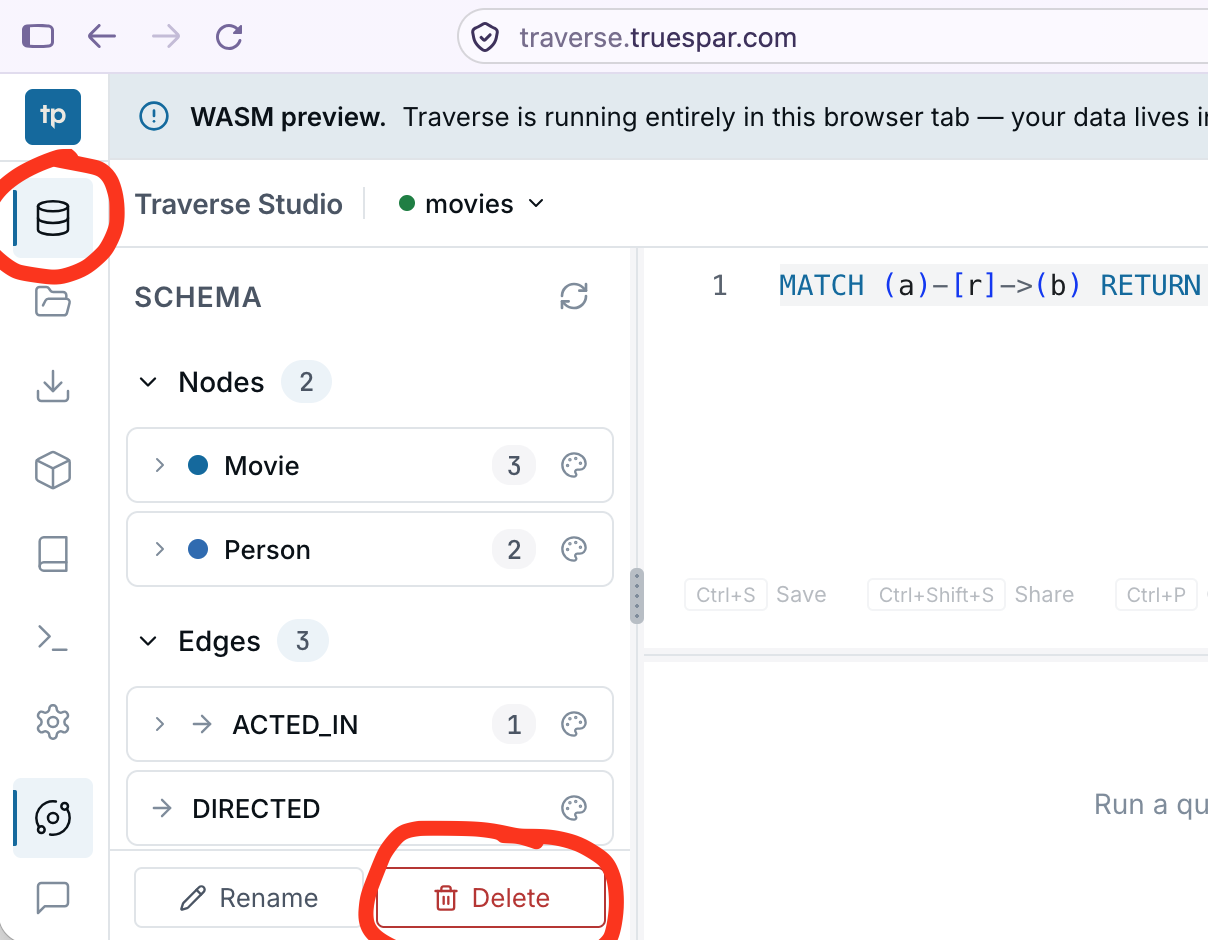
\includegraphics[height=\paperheight]{images/traverse-setup1.png}};
    \end{tikzpicture}
\end{frame}
\inlineslide{s:traverse-setup1}{}\label{l:traverse-setup1}

\begin{frame}[plain]
    \label{s:traverse-setup2}
    \begin{tikzpicture}[remember picture,overlay]
        \node at (current page.center) {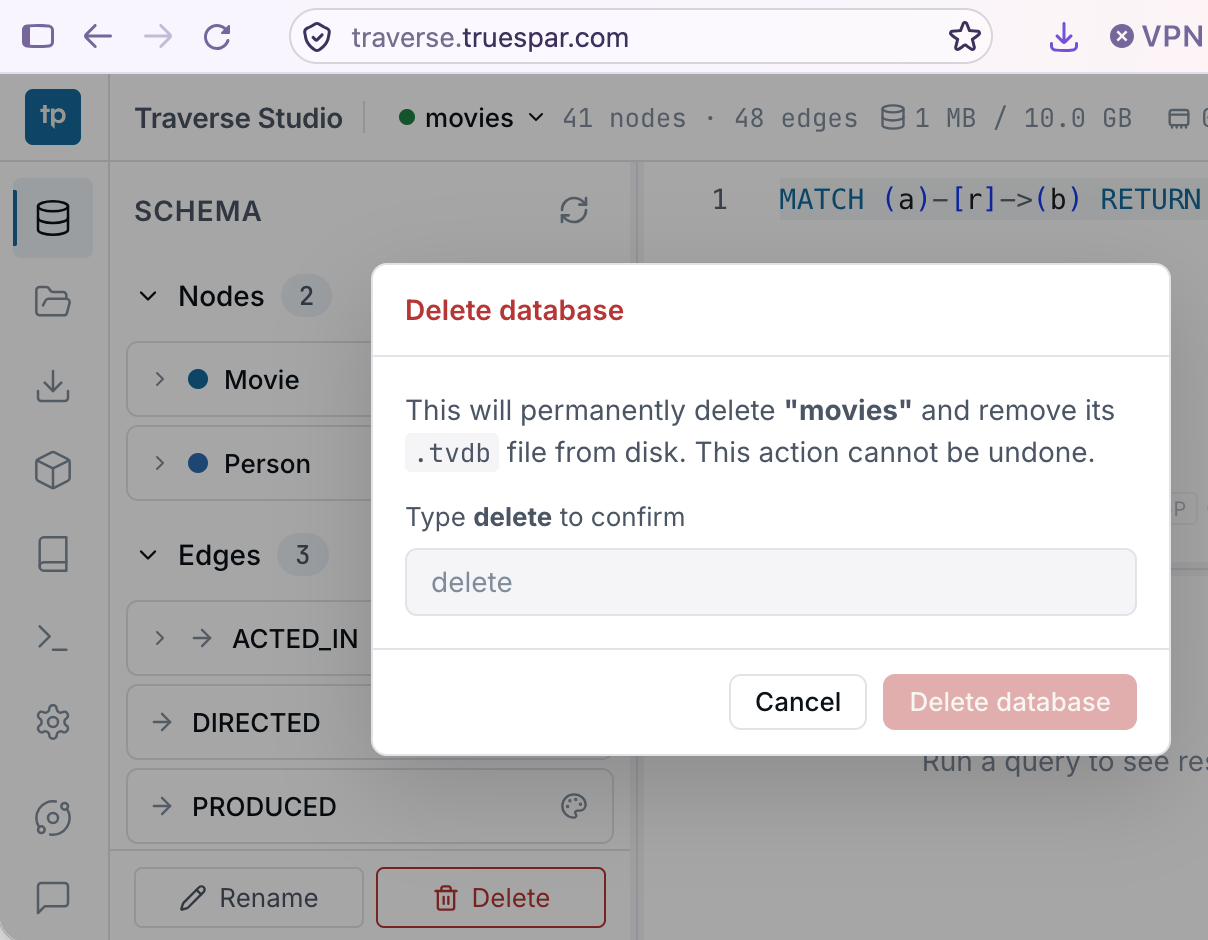
\includegraphics[height=\paperheight]{images/traverse-setup2.png}};
    \end{tikzpicture}
\end{frame}
\inlineslide{s:traverse-setup2}{}\label{l:traverse-setup2}

\begin{frame}[plain]
    \label{s:traverse-setup3}
    \begin{tikzpicture}[remember picture,overlay]
        \node at (current page.center) {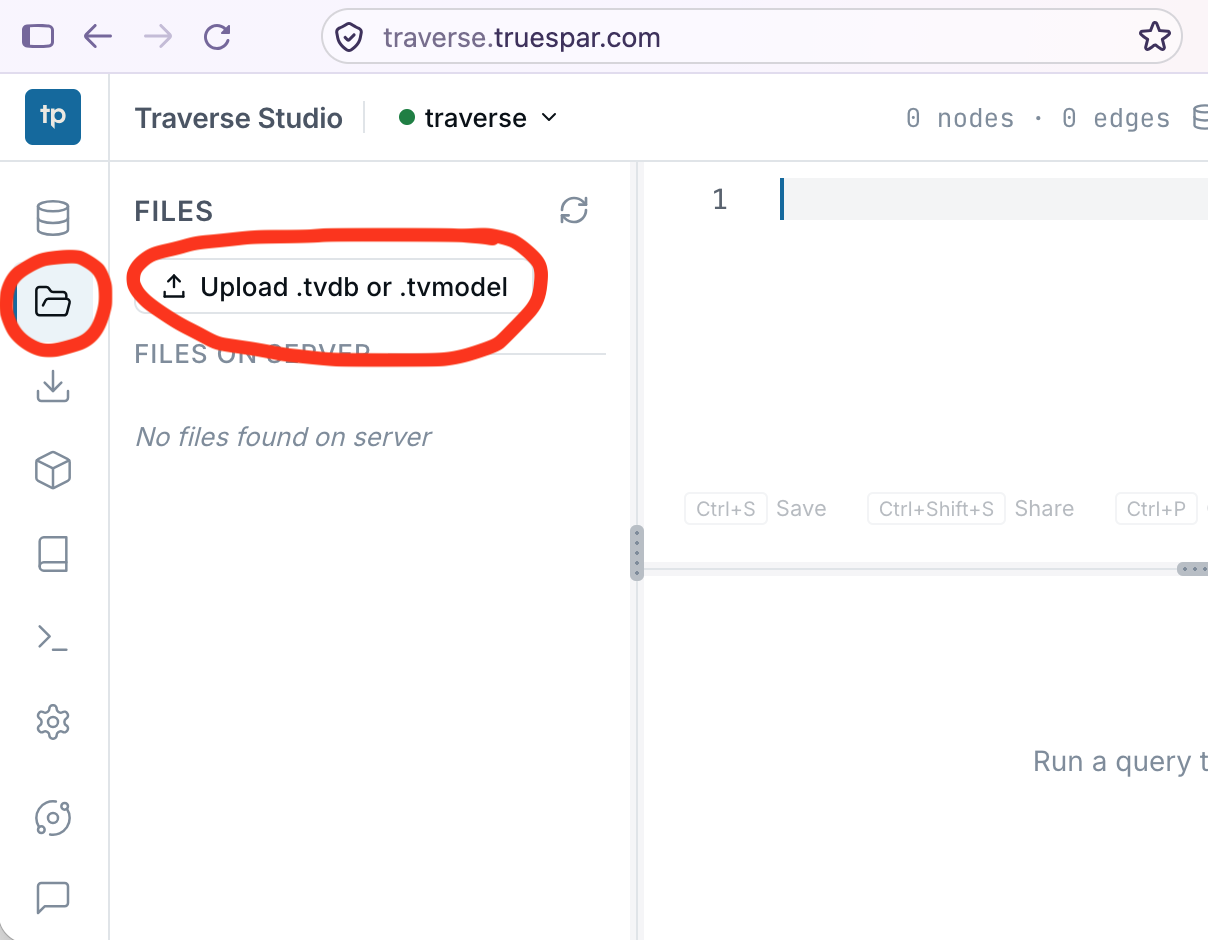
\includegraphics[height=\paperheight]{images/traverse-setup3.png}};
    \end{tikzpicture}
\end{frame}
\inlineslide{s:traverse-setup3}{}\label{l:traverse-setup3}


\subsection{Querying graphs with Cypher}\label{sec:cypher}

\emph{Cypher} is a declarative query language for property graphs, originally developed for Neo4j and now implemented by many graph databases \citep{Francis2018}.
The central idea of Cypher is \emph{pattern matching}: a query describes the shape of the part of the graph it is looking for, using a syntax that looks like a drawing of the graph in ASCII characters, and the database finds all the places in the graph where that pattern occurs.

The simplest pattern is a single vertex, as shown on \autoref{l:cypher-match}.
A vertex is written in round brackets, like a circle: \code{(m:Movie)} matches any vertex with the label \code{Movie}, and gives it the name \code{m}, so that the rest of the query can refer to it (much like a table alias in SQL).
The properties in curly braces restrict the match to vertices with those property values.
\code{RETURN} plays the role of SQL's \code{SELECT}: it says what to output for each match.
As in SQL, a condition can also be written in a \code{WHERE} clause, and the two forms on the slide are equivalent.

\begin{frame}
    \label{s:cypher-match}
    \frametitle{Cypher: matching a vertex}
    \inputminted[fontsize=\footnotesize]{cypher}{code/graph-match.cypher}
    \vspace{0.3em}
    {\footnotesize% Result of the first MATCH example on s:cypher-match
% Generated from graph-match.cypher by examples/render.py -- do not edit.
% Regenerate with: make examples
\begin{tabular}{|l|r|l|}\hline
    \textbf{m.title} & \textbf{m.year} & \textbf{m.genres} \\\hline
    The Kid & 1921 & [Comedy, Drama, Family] \\\hline
\end{tabular}%
}\\[0.8em]
    \code{(m:Movie)}: vertex with label \code{Movie}, called \code{m}\\
    \code{{title: ...}}: properties that must match\\[0.8em]\pause
    Equivalently, with \code{WHERE}:
    \inputminted[fontsize=\footnotesize]{cypher}{code/graph-where.cypher}
\end{frame}
\inlineslide{s:cypher-match}{}\label{l:cypher-match}

Patterns become more interesting when they include edges.
An edge is written in square brackets between two vertices, with dashes and an arrowhead showing its direction: \code{(p)-[:DIRECTED]->(m)} matches an edge of type \code{DIRECTED} from \code{p} to \code{m}.
The query on \autoref{l:cypher-edges} finds the movies directed by Steven Spielberg, by matching the person with that name, following the \code{DIRECTED} edges out of that vertex, and returning the movie at the other end of each.
An edge can also be given a name, such as \code{r} in the query on \autoref{l:cypher-edge-props}, and then its properties can be used in the same way as those of a vertex.

\begin{frame}
    \label{s:cypher-edges}
    \frametitle{Cypher: matching edges}
    Which movies did Steven Spielberg direct?
    \inputminted[fontsize=\footnotesize]{cypher}{code/graph-directed.cypher}
    \vspace{0.3em}
    {\footnotesize% Result of the Cypher query on s:cypher-edges
% Generated from graph-directed.cypher by examples/render.py -- do not edit.
% Regenerate with: make examples
\begin{tabular}{|l|r|}\hline
    \textbf{m.title} & \textbf{m.year} \\\hline
    Jaws & 1975 \\
    Close Encounters of the Third Kind & 1977 \\
    Raiders of the Lost Ark & 1981 \\
    E.T. the Extra-Terrestrial & 1982 \\\hline
\end{tabular}%
}\\[0.8em]
    \code{(p)-[:DIRECTED]->(m)}: edge of type \code{DIRECTED} from \code{p} to \code{m}
\end{frame}
\inlineslide{s:cypher-edges}{}\label{l:cypher-edges}

\begin{frame}
    \label{s:cypher-edge-props}
    \frametitle{Cypher: properties of edges}
    Give the edge a name (\code{r}) to use its properties:
    \inputminted[fontsize=\footnotesize]{cypher}{code/graph-roles.cypher}
    \vspace{0.3em}
    {\footnotesize% Result of the query with relationship properties on s:cypher-edges
% Generated from graph-roles.cypher by examples/render.py -- do not edit.
% Regenerate with: make examples
\begin{tabular}{|l|l|}\hline
    \textbf{p.name} & \textbf{r.roles} \\\hline
    Albert Austin & [Car Thief, Man in Shelter] \\
    B.F. Blinn & [His Assistant] \\
    Beulah Bains & [Bride] \\
    Carl Miller & [The Man] \\\hline
\end{tabular}%
}\\[0.8em]\pause
    \code{(p)<-[:DIRECTED]-(m)}: edge from \code{m} to \code{p}\\
    \code{(p)-[:DIRECTED]-(m)}: edge in either direction\\
    \code{(p)-->(m)}: edge of any type from \code{p} to \code{m}
\end{frame}
\inlineslide{s:cypher-edge-props}{}\label{l:cypher-edge-props}

The direction of an edge in a pattern matters: \code{(p)<-[:DIRECTED]-(m)} would look for edges from the movie to the person, of which there are none in our graph.
If the direction doesn't matter, the arrowhead can be left out, as in \code{(p)-[:DIRECTED]-(m)}, which matches edges in either direction.
And if the type of the edge doesn't matter, it can be left out too: \code{(p)-->(m)} matches an edge of any type from \code{p} to \code{m}.

\autoref{l:cypher-vs-sql} shows the first query of \autoref{l:cypher-edges} side by side with a SQL query that returns the same result from the relational database.
Each edge in the Cypher pattern corresponds to a join through the \code{has_position} table in SQL.
The Cypher query is shorter, and arguably easier to read, because the pattern shows the shape of the data that we are looking for.
But the two queries are doing essentially the same thing, and a graph query can always be translated into SQL; the difference lies in how convenient it is to write, and potentially how efficiently the database can execute it.

\begin{frame}
    \label{s:cypher-vs-sql}
    \frametitle{Cypher compared to SQL}
    \textbf{Cypher}:
    \inputminted[fontsize=\footnotesize]{cypher}{code/graph-directed.cypher}
    \vspace{0.6em}
    \textbf{SQL} (same result):
    \inputminted[fontsize=\footnotesize]{sql}{code/graph-directed.sql}
    \vspace{0.6em}
    An edge in a pattern $\approx$ a join through \code{has_position}
\end{frame}
\inlineslide{s:cypher-vs-sql}{}\label{l:cypher-vs-sql}

A pattern can contain any number of vertices and edges.
The query on \autoref{l:cypher-costars} finds pairs of actors who have acted together, by matching two \code{ACTED_IN} edges that point to the same movie \code{m}, and counts the movies that each pair has in common.
The \code{WHERE} condition \code{p1.person_id < p2.person_id} ensures that each pair is counted only once: without it, every pair would appear twice (once in each order), and every actor would be paired with themselves too.

Cypher has aggregate functions like those in SQL, but no \code{GROUP BY} clause.
Instead, the grouping is implicit: the expressions in the \code{RETURN} clause that are not aggregates are the grouping keys.
So in this query, the results are grouped by \code{name1} and \code{name2}, and \code{count(*)} counts the matches in each group, much like the SQL query in \autoref{q:costars-sql}.
(As the results show, our example database contains only the most prominent members of each cast, so the counts are lower than you might expect.)

\begin{frame}
    \label{s:cypher-costars}
    \frametitle{Longer patterns and aggregation}
    Which pairs of actors have appeared together most often?
    \inputminted[fontsize=\footnotesize]{cypher}{code/graph-costars.cypher}
    \vspace{0.3em}
    {\footnotesize% Result of the co-actor query on s:cypher-costars
% Generated from graph-costars.cypher by examples/render.py -- do not edit.
% Regenerate with: make examples
\begin{tabular}{|l|l|r|}\hline
    \textbf{name1} & \textbf{name2} & \textbf{movies} \\\hline
    Daniel Radcliffe & Emma Watson & 8 \\
    Rupert Grint & Daniel Radcliffe & 8 \\
    Rupert Grint & Emma Watson & 8 \\
    Johnny Depp & Helena Bonham Carter & 7 \\
    Robert Downey Jr. & Scarlett Johansson & 7 \\\hline
\end{tabular}%
}\\[0.8em]\pause
    No \code{GROUP BY}: the non-aggregated expressions in \code{RETURN} are the grouping keys
\end{frame}
\inlineslide{s:cypher-costars}{}\label{l:cypher-costars}

\supervision{\label{q:cypher-queries}
    Write Cypher queries over the graph version of the example database to answer the following questions.
    \begin{enumerate}
        \item Which movies did Charles Chaplin both direct and act in?
        \item Who are the five people who composed the music for the most movies?
        \item On which movies did both Lana Wachowski and Lilly Wachowski work, in any position?
    \end{enumerate}
}{
    \begin{enumerate}
        \item The pattern needs two edges from Chaplin to the same movie, which we can express by using the variable \code{m} twice:
            \inputminted[fontsize=\small]{cypher}{code/q-graph-chaplin.cypher}
            \begin{quote}% Result of code/q-graph-chaplin.cypher, for the solution to q:cypher-queries
% Generated from graph-q-chaplin.cypher by examples/render.py -- do not edit.
% Regenerate with: make examples
\begin{tabular}{|l|r|}\hline
    \textbf{m.title} & \textbf{m.year} \\\hline
    The Kid & 1921 \\
    The Gold Rush & 1925 \\
    City Lights & 1931 \\
    Modern Times & 1936 \\
    The Great Dictator & 1940 \\\hline
\end{tabular}%
\end{quote}
            It would be equally valid to write the pattern as two comma-separated parts, \code{(p:Person {name: 'Charles Chaplin'})-[:DIRECTED]->(m:Movie), (p)-[:ACTED_IN]->(m)}.
        \item Counting the \code{COMPOSED_FOR} edges of each person, with the person's name as the implicit grouping key:
            \inputminted[fontsize=\small]{cypher}{code/q-graph-composers.cypher}
            \begin{quote}% Result of code/q-graph-composers.cypher, for the solution to q:cypher-queries
% Generated from graph-q-composers.cypher by examples/render.py -- do not edit.
% Regenerate with: make examples
\begin{tabular}{|l|r|}\hline
    \textbf{p.name} & \textbf{movies} \\\hline
    Hans Zimmer & 72 \\
    James Newton Howard & 52 \\
    Danny Elfman & 49 \\
    John Williams & 48 \\
    Marco Beltrami & 42 \\\hline
\end{tabular}%
\end{quote}
            Grouping by name would merge two different composers who happen to have the same name; returning \code{p.person_id} as well would make it group by person.
        \item An edge of any type is written \code{-->}:
            \inputminted[fontsize=\small]{cypher}{code/q-graph-wachowskis.cypher}
            \begin{quote}% Result of code/q-graph-wachowskis.cypher, for the solution to q:cypher-queries
% Generated from graph-q-wachowskis.cypher by examples/render.py -- do not edit.
% Regenerate with: make examples
\begin{tabular}{|l|r|}\hline
    \textbf{m.title} & \textbf{m.year} \\\hline
    Bound & 1996 \\
    The Matrix & 1999 \\
    The Animatrix & 2003 \\
    The Matrix Reloaded & 2003 \\
    The Matrix Revolutions & 2003 \\
    V for Vendetta & 2005 \\
    Cloud Atlas & 2012 \\
    The Matrix Resurrections & 2021 \\\hline
\end{tabular}%
\end{quote}
            \code{DISTINCT} is needed because each of them may have held several positions on the same movie (directing and writing it, say), and each combination of edges is a separate match.
    \end{enumerate}
}

\supervision{\label{q:costars-sql}
    Write a SQL query over the relational version of the example database that returns the same result as the Cypher query that finds the pairs of actors who have appeared together most often.
    Compare the two queries.
}{
    Each \code{ACTED_IN} edge in the pattern corresponds to a row of \code{has_position} with \code{position = 'actor'}, so we join \code{has_position} with itself on the movie, and join \code{people} twice to get the names:
    \inputminted[fontsize=\small]{sql}{code/q-costars.sql}
    \begin{quote}% Result of code/q-costars.sql, for the solution to q:costars-sql
% Generated from q-costars.sql by examples/render.py -- do not edit.
% Regenerate with: make examples
\begin{tabular}{|l|l|r|}\hline
    \textbf{name1} & \textbf{name2} & \textbf{movies} \\\hline
    Daniel Radcliffe & Emma Watson & 8 \\
    Rupert Grint & Daniel Radcliffe & 8 \\
    Rupert Grint & Emma Watson & 8 \\
    Johnny Depp & Helena Bonham Carter & 7 \\
    Robert Downey Jr. & Scarlett Johansson & 7 \\\hline
\end{tabular}%
\end{quote}
    This is the same result as the Cypher query.
    The SQL needs four tables, and four join conditions that the reader has to piece together to see that the query is about two people connected through a movie, whereas the Cypher pattern shows this shape directly.
    The SQL query also has to name the grouping columns explicitly, including \code{person_id}, so that two different people with the same name are not merged; the Cypher query groups by names only, so it would merge them.
    (It does not need the \code{movies} table at all, since the movie ID in \code{has_position} is enough to match the two actors.)
}


\subsection{Paths of variable length}\label{sec:graph-paths}

The patterns we have seen so far have a fixed number of edges.
But many questions about graphs involve paths whose length is not known in advance: how are two people connected, and through how many intermediaries?
A well-known example is the game ``Six degrees of Kevin Bacon'', in which the challenge is to connect any actor to the actor Kevin Bacon through as short a chain as possible of actors who have appeared in the same movie.

In Cypher, an edge pattern can be followed by an asterisk and a number, as shown on \autoref{l:var-length}, to match a path of that many edges.
Since \code{ACTED_IN} edges go from people to movies, a path from one actor to another alternates between people and movies, and so it always has an even number of edges.
For example, between the actors Jennifer Lawrence and Daniel Radcliffe there are \graphpathstwo\ paths of two \code{ACTED_IN} edges (they have not appeared in the same movie in our database), \graphpathsfour\ paths of four edges, and \graphpathssix\ of six.
The direction of the edges is left out of the pattern, since the path goes from Lawrence to a movie along an \code{ACTED_IN} edge, and then from that movie to another actor against the direction of an \code{ACTED_IN} edge.
A range such as \code{*2..6} matches paths with between two and six edges, and an asterisk on its own matches paths of any length, though that could be a very large number of paths.

\begin{frame}
    \label{s:var-length}
    \frametitle{Paths of variable length}
    \inputminted[fontsize=\footnotesize]{cypher}{code/graph-varlength.cypher}
    \vspace{0.3em}
    $\Rightarrow$ \graphpathsfour\ paths\\[0.8em]
    \code{[:ACTED_IN*4]}: path of 4 \code{ACTED_IN} edges, in either direction\\[0.3em]
    \hspace*{1em}\code{*2}: \graphpathstwo\ paths\quad \code{*6}: \graphpathssix\ paths\\[0.3em]
    \code{*2..6}: between 2 and 6 edges; \code{*}: any number\\[0.8em]\pause
    Actor $\rightarrow$ movie $\leftarrow$ actor $\rightarrow$ movie $\leftarrow$ actor\\
    so a path between actors has an \textbf{even} number of edges
\end{frame}
\inlineslide{s:var-length}{}\label{l:var-length}

Usually we want the shortest such path, and graph databases have efficient algorithms for finding it, such as breadth-first search.
In Cypher, the \code{shortestPath} function finds one shortest path matching a pattern, as shown on \autoref{l:shortest-path}.
The query then uses \code{nodes(path)}, which is the list of the vertices along the path, to return one row per vertex, so that we can see the people and movies that connect the two actors.

The GQL standard, which we discuss in \autoref{sec:gql}, introduced a different syntax for shortest paths, shown on \autoref{l:gql}.

\begin{frame}
    \label{s:shortest-path}
    \frametitle{Shortest paths}
    \inputminted[fontsize=\footnotesize]{cypher}{code/graph-shortest.cypher}
    \vspace{0.3em}
    {\footnotesize% Result of the shortest-path query on s:shortest-path
% Generated from graph-shortest.cypher by examples/render.py -- do not edit.
% Regenerate with: make examples
\begin{tabular}{|r|l|}\hline
    \textbf{step} & \textbf{vertex} \\\hline
    0 & Jennifer Lawrence \\
    1 & Mother! \\
    2 & Domhnall Gleeson \\
    3 & Harry Potter and the Deathly Hallows: Part 2 \\
    4 & Daniel Radcliffe \\\hline
\end{tabular}%
}
\end{frame}
\inlineslide{s:shortest-path}{}\label{l:shortest-path}

Finally, we can compute the \emph{Bacon number} of every actor: the number of movies in the shortest chain that connects them to Kevin Bacon.
The query on \autoref{l:bacon} uses \code{allShortestPaths}, which finds the shortest paths from Kevin Bacon to every other person who can be reached through \code{ACTED_IN} edges.
Since each step from one actor to the next consists of two edges, the Bacon number is half the length of the path.
The result shows how many people have each Bacon number; the actors who are missing from the result cannot be connected to Kevin Bacon at all in our database.

In SQL, a query like this one is possible, but much harder to write: since the length of the path is not known in advance, we can't simply write a fixed number of joins.
SQL needs recursive queries to do this, which we will look at in a later lecture.
Queries that follow paths of variable length are the area in which graph query languages have the clearest advantage over SQL.

\begin{frame}
    \label{s:bacon}
    \frametitle{Bacon numbers}
    \begin{columns}[T,onlytextwidth]
        \begin{column}{0.6\textwidth}
            \inputminted[fontsize=\scriptsize]{cypher}{code/graph-bacon.cypher}
        \end{column}
        \begin{column}{0.38\textwidth}
            {\scriptsize% Result of the Bacon number query on s:bacon
% Generated from graph-bacon.cypher by examples/render.py -- do not edit.
% Regenerate with: make examples
\begin{tabular}{|r|r|}\hline
    \textbf{bacon\_number} & \textbf{people} \\\hline
    1 & 107 \\
    2 & 3,519 \\
    3 & 8,631 \\
    4 & 1,676 \\
    5 & 364 \\
    6 & 212 \\
    7 & 62 \\
    8 & 9 \\\hline
\end{tabular}%
}
        \end{column}
    \end{columns}
    \vspace{1em}
    \textbf{Bacon number}: number of movies in the shortest chain connecting an actor to Kevin Bacon\\[0.8em]\pause
    In SQL: the number of joins depends on the data\\
    $\Rightarrow$ needs a \textbf{recursive} query (later lecture)
\end{frame}
\inlineslide{s:bacon}{}\label{l:bacon}


\subsection{Graph query languages}\label{sec:gql}

Cypher was created at Neo4j around 2011, and was later published as an open specification, called openCypher, so that other databases could implement it.
Several other graph query languages have also been used, such as SPARQL for a different graph data model called RDF, and Gremlin, in which a query is written as a sequence of traversal steps.
To bring order to this variety, the ISO committee that maintains the SQL standard has developed two related standards for querying property graphs, based to a large extent on Cypher \citep{Deutsch2022}.

\emph{GQL} (Graph Query Language), published in 2024 as ISO/IEC 39075, is a stand-alone query language for graph databases; Traverse supports GQL as well as Cypher.
Most of GQL looks like Cypher, but there are differences: for example, the query on \autoref{l:gql} finds the shortest path between two actors like the one on \autoref{l:shortest-path}, writing \code{SHORTEST 1} before the pattern to ask for one shortest path, and \code{-[:ACTED_IN]-+} to mean a path of one or more \code{ACTED_IN} edges.
\emph{SQL/PGQ} (Property Graph Queries), published in 2023 as part 16 of the SQL standard, adds graph pattern matching to SQL.
In SQL/PGQ, a property graph is defined as a \emph{view} over existing relational tables, specifying which tables contain vertices and which contain edges, and then graph patterns can be used in a SQL query through the \code{GRAPH_TABLE} construct.

\begin{frame}
    \label{s:gql}
    \frametitle{Graph query languages}
    \textbf{Cypher}: created at Neo4j; open specification (openCypher)\\[0.5em]
    Others: SPARQL (RDF triple stores), Gremlin, \dots\\[1em]\pause
    ISO standards, based largely on Cypher:
    \begin{itemize}
        \item \textbf{GQL}: graph query language (ISO/IEC 39075:2024)
        \item \textbf{SQL/PGQ}: graph pattern matching inside SQL (SQL:2023 part 16)\\[1em]\pause
    \end{itemize}
    GQL syntax for the shortest path between two actors:
    \inputminted[fontsize=\footnotesize]{cypher}{code/graph-shortest-gql.cypher}
\end{frame}
\inlineslide{s:gql}{}\label{l:gql}

This means that you don't necessarily need a graph database in order to run graph queries: a relational database that supports SQL/PGQ can treat its tables as a graph.
\autoref{l:sql-pgq} shows an example using the \code{duckpgq} extension for DuckDB, which you can install in the DuckDB command line on your own machine with the first two statements on the slide.
The \code{CREATE PROPERTY GRAPH} statement declares that rows of \code{movies} and \code{people} are vertices, and that each row of \code{plays_role} is an edge from the person to the movie identified by its foreign keys.
The query then matches a pattern in the \code{GRAPH_TABLE} construct, and the \code{COLUMNS} clause turns the matches into a table, which the rest of the SQL query can use like any other table.
It returns the same result as the three-table join on \autoref{l:multi-join}.

\begin{frame}
    \label{s:sql-pgq}
    \frametitle{SQL/PGQ in DuckDB}
    \inputminted[fontsize=\scriptsize]{sql}{code/pgq-create.sql}
    \vspace{0.3em}
    \inputminted[fontsize=\scriptsize]{sql}{code/pgq-query.sql}
    \vspace{0.3em}
    {\scriptsize% Result of the three-table join on s:multi-join
% Generated from sql-join3.sql by examples/render.py -- do not edit.
% Regenerate with: make examples
\begin{tabular}{|l|l|l|}\hline
    \textbf{title} & \textbf{role} & \textbf{name} \\\hline
    The Kid & A Tramp & Charles Chaplin \\
    The Kid & Bride & Beulah Bains \\
    The Kid & Car Thief & Albert Austin \\
    The Kid & His Assistant & B.F. Blinn \\\hline
\end{tabular}%
}\\[0.5em]
    {\footnotesize Same result as the three-table join in SQL}
\end{frame}
\inlineslide{s:sql-pgq}{}\label{l:sql-pgq}


\subsection{Comparing the data models}\label{sec:graph-tradeoffs}

We have now represented the same data in three data models, and \autoref{l:model-comparison} summarises how they compare.
Graphs have the most flexible structure: any vertex can be related to any other, so many-to-many relationships need no join tables, and a new type of relationship can be added just by creating edges of a new type, without any schema migration.
Graph query languages make it easy to express patterns of relationships, and especially to follow paths of variable length.
Graph databases are designed so that following the edges from a vertex to its neighbours is efficient, which matters for queries that traverse many edges.

On the other hand, the relational model, with its enforced schema and its normalisation, is better at guaranteeing the integrity of the data, and SQL is a more widely known language that is very good at aggregating large numbers of rows, which is what analytics queries mostly do.
And the document model is the most convenient when the data is a collection of self-contained trees that are usually read and written as a whole.
As always, there is no single best choice; and with JSON support and SQL/PGQ, a single relational database can increasingly support all three models.

\begin{frame}
    \label{s:model-comparison}
    \frametitle{Relational, document, and graph}
    \footnotesize
    \rowcolors[]{2}{}{blue!10}
    \renewcommand{\arraystretch}{1.4}
    % Four columns need the padding reduced to fit: 1.9 + 3 x 2.35cm, plus 8 x 4pt.
    \setlength{\tabcolsep}{4pt}
    \begin{tabular}{>{\raggedright}p{1.9cm}|>{\raggedright}p{2.35cm}|>{\raggedright}p{2.35cm}|>{\raggedright\arraybackslash}p{2.35cm}}
        \hline
        & \textbf{Relational} & \textbf{Document} & \textbf{Graph} \\\hline
        Structure & flat tables & trees & vertices and edges \pause\\
        Many-to-many & join table & copies or IDs & edges \pause\\
        Schema & enforced on write & implicit & usually implicit \pause\\
        Best for & integrity, aggregation & self-contained records & connections, paths \pause\\
        Language & SQL & SQL with JSON, MongoDB, \dots & Cypher, GQL, SQL/PGQ \\\hline
    \end{tabular}
\end{frame}
\inlineslide{s:model-comparison}{}\label{l:model-comparison}

\supervision{\label{q:genre-nodes}
    In the graph version of the example database, each movie's genres are a list of strings in its \code{genres} property.
    An alternative design would be to make each genre a vertex with the label \code{Genre}, and to connect each movie to its genres with \code{HAS_GENRE} edges.
    For each design, write a Cypher query that counts the movies that are both romantic and comedies (that is, have both the Romance and the Comedy genres).
    What are the advantages and disadvantages of each design?
}{
    With genres as a list property, the \code{IN} operator tests whether a list contains a value:
    \inputminted[fontsize=\small]{cypher}{code/q-graph-romcom-list.cypher}
    which returns % Result of code/q-graph-romcom-list.cypher, for the solution to q:genre-nodes
% Generated from graph-q-romcom.cypher by examples/render.py -- do not edit.
% Regenerate with: make examples
174%
.
    With genres as vertices, the pattern connects the movie to both genre vertices:
    \inputminted[fontsize=\small]{cypher}{code/q-graph-romcom-nodes.cypher}
    which returns the same count.
    (The genre vertices could be created from the list properties with the following query, which uses \code{MERGE} to create each genre vertex only the first time that genre is encountered:)
    \inputminted[fontsize=\small]{cypher}{code/q-graph-genre-nodes.cypher}

    Advantages of genre vertices:
    \begin{itemize}
        \item Each genre's name is stored only once, which is the normalised design: renaming a genre changes one vertex, and a genre can exist (and have properties of its own, such as a description) even if no movie has it yet.
        \item Queries can start from a genre and follow its edges to its movies, which can be efficient if the database indexes the edges of each vertex, and they can follow paths through genres (such as movies that share a genre with a given movie) in the same way as through people.
    \end{itemize}
    Advantages of the list property:
    \begin{itemize}
        \item It is simpler: reading a movie gives its genres without following any edges, as in the document model.
        \item The graph has fewer vertices and edges: there are \graphmovies\ movies, but the edge-based design needs an edge for every pairing of a movie and a genre.
    \end{itemize}
    This is the same trade-off between normalised and denormalised representations that we saw in the document model, and the relational schema made the same choice as the genre vertices, with its \code{genres} and \code{has_genre} tables.
}

\footnotesize
\bibliographystyle{plainnat}
\bibliography{references}{}
\end{document}
